%% The following is a directive for TeXShop to indicate the main file
%%!TEX root = diss.tex

\chapter{Towards Efficient Resolution of Thue-Mahler Equations}
\label{ch:TMs} \edit{label}

Let $a \in \mathbb{Z}$ be nonzero, let $S=\{p_1,\dotsc,p_v\}$ be a set of rational primes, and let $F \in \mathbb{Z}[X,Y]$ be irreducible and homogeneous of degree $n \geq 3$. We consider the classical Thue--Mahler equation
\begin{equation} \label{Eq:TM1}
F(X,Y) = a p_1^{Z_1}\cdots p_v^{Z_v}, \quad (X,Y) \in \mathbb{Z}^2,
\end{equation}
where
\[F(X,Y) = c_0 X^n + c_1 X^{n-1}Y + \cdots + c_{n-1}XY^{n-1} + c_nY^n.\]
and $\gcd(X,Y)=1$. 

We would like to enumerate the set of solutions $\{X,Y, Z_1, \dots, Z_v\}$ of \eqref{Eq:TM1}, where $Z_i \geq 0$ for $i = 1, \dots, v$. Solutions to this equation having $(X,Y) = 1$ and $n = 3$ correspond to elliptic curves with good reduction outside of $\{p_1, \dots, p_v\}$. The algorithm of Tzanakis, de Weger generates solutions $(X,Y)$ in the case 
\[(X,Y) = 1, \quad (a, p_1, \dots, p_v) = 1, \quad (Y,c_0) = 1.\]
To implement this algorithm for our specific application, we modify our Thue-Mahler equation so that we are reduced to the case where
\[(X,Y) = 1, \quad (a, p_1, \dots, p_v) = 1, \quad c_0 = 1.\]
The solutions corresponding to these conditions are then converted back into solutions of the original Thue-Mahler equation. The remainder of this section outlines these modifications. 

%---------------------------------------------------------------------------------------------------------------------------------------------%
%---------------------------------------------------------------------------------------------------------------------------------------------%

\subsection{Reducing to $(a, p_1, \dots, p_v) = 1$ and $c_0 = 1$}
%---------------------------------------------------------------------------------------------------------------------------------------------%
%---------------------------------------------------------------------------------------------------------------------------------------------%

\section{The Relevant Algebraic Number Field}
Now, for each $c$, we solve
\[f(x,y) = x^n + C_1 x^{n-1}y + \dots + C_{n-1}xy^{n-1} + C_ny^n = c p_1^{z_1} \cdots p_v^{z_v}.\]
Here, 
\[\gcd(x,y) = 1 \quad \text{ and } \quad \gcd(c,p_1, \dots, p_v) = 1.\]
In our case, $n = 3$ and so
\[f(x,y) = x^3 + C_1 x^{2}y + C_2xy^2 + C_3y^3 = c p_1^{z_1} \cdots p_v^{z_v}.\]

Following the Thue-Mahler solver algorithm, put
\[g(t) = F(t,1) = t^3 + C_1t^2 + C_2t + C_3\]
and note that $g(t)$ is irreducible in $\mathbb{Z}[t]$. Let $K = \mathbb{Q}(\theta)$ with $g(\theta) = 0$. Then \eqref{Eq:TM2} is equivalent to solving finitely many equations of the form
\begin{equation} \label{Eq:norm}
N_{K/\mathbb{Q}}(x-y\theta) = cp_1^{z_1}\dots p_v^{z_v}
\end{equation}
for each distinct value of $c$. 

%---------------------------------------------------------------------------------------------------------------------------------------------%
%---------------------------------------------------------------------------------------------------------------------------------------------%

\section{Decomposition of Primes}

Let $p_i$ be any rational prime and let 
\[(p_i)\mathcal{O}_K = \prod_{j = 1}^{m_i} \mathfrak{p}_{ij}^{e_{ij}}\]
be the factorization of $p_i$ into prime ideals in the ring of integers $\mathcal{O}_K$ of $K$. Let $f_{ij}$ be the residue degree of $\mathfrak{p}_{ij}$ over $p_i$. We have $\deg(g_i(t)) = e_{ij}f_{ij}$.

Let
\[g(t) = g_{i1}(t)\cdots g_{im}(t)\]
be the decomposition of $g(t)$ into irreducible polynomials $g_{ij}(t) \in \mathbb{Q}_{p_i}[t]$. The prime ideals in $K$ dividing $p_i$ are in one-to-one correspondence with $g_{i1}(t), \dots, g_{im}(t)$, and in particular, $\deg(g_{ij}(t)) = e_{ij}f_{ij}$. 

Then, since $N(\mathfrak{p}_{ij}) = p_i^{f_{ij}}$, \eqref{Eq:norm} leads to finitely many ideal equations of the form
\begin{equation} \label{Eq:ideals}
(x-y\theta)\mathcal{O}_K = \mathfrak{a} \prod_{j = 1}^{m_1} \mathfrak{p}_{1j}^{z_{1j}} \cdots \prod_{j = 1}^{m_v} \mathfrak{p}_{vj}^{z_{vj}}
\end{equation}
where $\mathfrak{a}$ is an ideal of norm $|c|$ (for each choice of $c$) and the $z_{ij}$ are unknown integers related to $z_i$ by $\sum_{j = 1}^{m_i} f_{ij}z_{ij} = z_i $. Thus
\[Z_i = z_i - \ord_p{u} - \ord_p(a) =  \sum_{j = 1}^{m_i} f_{ij}z_{ij} -  \ord_p{u} - \ord_p(a).\]

Our first task is to cut down the number of variables appearing in \eqref{Eq:ideals}. We will do this by showing that only a few prime ideals can divide $(x-y\theta)\mathcal{O}_K$ to a large power. 

%---------------------------------------------------------------------------------------------------------------------------------------------%
%---------------------------------------------------------------------------------------------------------------------------------------------%
%---------------------------------------------------------------------------------------------------------------------------------------------%
\section{Factorization of the Thue-Mahler Equation}

%---------------------------------------------------------------------------------------------------------------------------------------------%
\subsection{Refinements}


%---------------------------------------------------------------------------------------------------------------------------------------------%

At this point, regardless of which method was used to compute $A$ and $\mathbf{r}$, we note that the ideal generated by $\alpha$ has norm
\[|c|\cdot p_1^{t_1 + r_1} \cdots p_{\nu}^{t_{\nu} + r_{\nu}}p_{\nu +1}^{t_{\nu +1}} \cdots p_v^{t_v}.\]
Now the $n_i$ are related to the $z_i$ via
\[z_i = u_i + t_i = \sum_{j = 1}^{\nu}n_ja_{ij} + r_i + t_i.\]
Hence
\[Z_i = z_i - \ord_p(u) - \ord_p(a) = \sum_{j = 1}^{\nu}n_ja_{ij} + r_i + t_i - \ord_p(u) - \ord_p(a) \]
Here, we note that $u_i = r_i = 0$ for all $i \in \{\nu + 1, \dots, v\}$. 


Fix a complete set of fundamental units of $\mathcal{O}_K: \varepsilon_1, \dots, \varepsilon_r$. Here $r = s + t -1$, where $s$ denotes the number of real embeddings of $K$ into $\mathbb{C}$ and $t$ denotes the number of complex conjugate pairs of non-real embeddings of $K$ into $\mathbb{C}$. Then
\begin{equation} \label{Eq:main2}
x-y\theta = \alpha \zeta \varepsilon_1^{a_1} \cdots \varepsilon_r^{a_r}\gamma_1^{n_1}\cdots \gamma_{\nu}^{n_{\nu}}
\end{equation}
with unknowns $a_i \in \mathbb{Z}$, $n_i \in \mathbb{Z}_{\geq 0}$, and $\zeta$ in the set $T$ of roots of unity in $\mathcal{O}_K$. Since $T$ is also finite, we will treat $\zeta$ as another parameter. Since $K$ is a degree $3$ extension of $\mathbb{Q}$, we either have $3$ real embeddings of $K$ into $\mathbb{C}$ (hence $s = 3$, $t = 0$ and $r = s+ t -1 = 3 + 0 -1 = 2$), or there is one real embedding of $K$ into $\mathbb{C}$ and a pair of complex conjugate embeddings of $K$ into $\mathbb{C}$ (hence $s = 1$, $t = 1$, and $r = s +t -1 = 1 + 1 -1 = 1$). 
That is, we have either  
\begin{equation} \label{Eq:main3}
x-y\theta = \alpha \zeta \varepsilon_1^{a_1} \cdot \gamma_1^{n_1}\cdots \gamma_{\nu}^{n_{\nu}}
\quad \text{ or } \quad 
x-y\theta = \alpha \zeta \varepsilon_1^{a_1} \varepsilon_2^{a_2}\cdot \gamma_1^{n_1}\cdots \gamma_{\nu}^{n_{\nu}}
\end{equation}

To summarize, our original problem of solving \eqref{Eq:TM1} has been reduced to the problem of solving finitely many equations of the form \eqref{Eq:main3} for the variables 
\[x,y, a_1, n_1, \dots, n_{\nu} \quad \text{ or } \quad x,y, a_1,a_2, n_1, \dots, n_{\nu} .\] 

From here, we deduce a so-called $S$-unit equation. In doing so, we eliminate the variables $x,y$ and set ourselves up to bound the exponents $a_1,n_1, \dots, n_{\nu}$, respectively $a_1,a_2,n_1, \dots, n_{\nu}$. We note here that generating the class group can be a timely computation. However, if we follow the method of Tzanakis-de Weger, we may be left with $h^{\nu}$ $S$-unit equations, all of which we would need to apply the principal ideal test to. That is to say, computing the class group is a faster operation than the alternative provided by Tzanakis-de Weger. 

%---------------------------------------------------------------------------------------------------------------------------------------------%
%---------------------------------------------------------------------------------------------------------------------------------------------%

\section{The $S$-Unit Equation}

Let $p \in \{p_1, \dots, p_v, \infty\}$. Denote the roots of $g(t)$ in $\overline{\mathbb{Q}_p}$ (where $\overline{\mathbb{Q}_{\infty}} = \overline{\mathbb{R}} = \mathbb{C}$) by $\theta^{(1)}, \theta^{(2)}, \theta^{(3)}$. Let $i_0, j, k \in \{1,2,3\}$ be distinct indices and consider the three embeddings of $K$ into $\overline{\mathbb{Q}_p}$ defined by $\theta \mapsto \theta^{(i_0)}, \theta^{(j)}, \theta^{(k)}$. We use $z^{(i)}$ to denote the image of $z$ under the embedding $\theta \mapsto \theta^{(i)}$. From the Siegel identity
\[\left(\theta^{(i_0)} - \theta^{(j)}\right)\left(x-y\theta^{(k)}\right) + \left(\theta^{(j)} - \theta^{(k)}\right)\left(x-y\theta^{(i_0)}\right) + \left(\theta^{(k)} - \theta^{(i_0)}\right)\left(x-y\theta^{(j)}\right) = 0,\]
applying these embeddings to $\beta = x-y\theta$ yields
\begin{equation}\label{Eq:Sunit}
\lambda = \delta_1 \prod_{i = 1}^r\left( \frac{\varepsilon_i^{(k)}}{\varepsilon_i^{(j)}}\right)^{a_i}\prod_{i = 1}^{\nu} \left( \frac{\gamma_i^{(k)}}{\gamma_i^{(j)}}\right)^{n_i} - 1 = \delta_2 \prod_{i = 1}^{r}\left( \frac{\varepsilon_i^{(i_0)}}{\varepsilon_i^{(j)}}\right)^{a_i} \prod_{i = 1}^{\nu} \left( \frac{\gamma_i^{(i_0)}}{\gamma_i^{(j)}}\right)^{n_i},
\end{equation}
where
\[\delta_1 = \frac{\theta^{(i_0)} - \theta^{(j)}}{\theta^{(i_0)} - \theta^{(k)}}\cdot\frac{\alpha^{(k)}\zeta^{(k)}}{\alpha^{(j)}\zeta^{(j)}}, \quad \delta_2 = \frac{\theta^{(j)} - \theta^{(k)}}{\theta^{(k)} - \theta^{(i_0)}}\cdot \frac{\alpha^{(i_0)}\zeta^{(i_0)}}{\alpha^{(j)}\zeta^{(j)}}\]
are constants and $r = 1$ or $r = 2$. 

Note that $\delta_1$ and $\delta_2$ are constants, in the sense that they do not rely on 
\[x, y, a_1, \dots, a_r,n_1, \dots, n_{\nu}.\]

%---------------------------------------------------------------------------------------------------------------------------------------------%
%---------------------------------------------------------------------------------------------------------------------------------------------%

\section{Specializing to Degree $3$}

We are interested in solving a Thue-Mahler equation of degree $3$. That is, 
\[F(X,Y) = c_0X^3 + c_1X^2Y + c_2XY^2 + c_3Y^3 = ap_1^{Z_1}\cdots p_v^{Z_v}.\]
Making the relevant changes as in the setup above (ie. reducing to a monic polynomial having solutions $(x,y) = 1$) and putting $g(t) = F(t,1)$ yields
\[g(t) = t^3 + C_1t^2 + C_2t + C_3,\]
an irreducible polynomial in $\mathbb{Z}[t]$. Then, setting $K = \mathbb{Q}(\theta)$ with $g(\theta) = 0$ yields a field $K$ of degree $3$ over $\mathbb{Q}$. Hence, the splitting field of $K$ is divisible by $3$. Since the Galois group is a subgroup of $S_3$, there are only two possibilities, namely $A_3$ or $S_3$. Recall that the discriminant of $g(t)$ is defined as 
\[D = C_1^2C_2^2 - 4C_2^3 - 4C_1^3C_3 - 27C_3^2 + 18C_1C_2C_3.\]

The Galois group of $g(t)$ is $A_3$ if and only if $D$ is a square. Explicitly, if $D$ is the square of an element of $\mathbb{Q}$, then the splitting field of the irreducible cubic $g(t)$ is obtained by adjoining any single root of $g(t)$ to $K$. The resulting field is Galois over $\mathbb{Q}$ of degree $3$ with cyclic group of order $3$ as Galois group. In particular, $K$ is the Galois group of $g(t)$. In this case, 
\[g(t) = (t - \theta_1)(t - \theta_2)(t - \theta_3)\]
in $K$, where $\theta_1, \theta_2, \theta_3 \in K$ and, without loss of generality, $\theta_1 = \theta$.  

If $D$ is not the square of an element of $\mathbb{Q}$, then the splitting field of $g(t)$ is of degree $6$ over $\mathbb{Q}$, hence is the field $K\left(\theta, \sqrt{D}\right)$ for any one of the roots $\theta$ of $g(t)$. This extension is Galois over $\mathbb{Q}$ with Galois group $S_3$. In this case, 
\[g(t) = (t - \theta)\tilde{g}(t)\]
in $K = \mathbb{Q}(\theta)$, where $\tilde{g}(t) \in K[t]$ is an irreducible degree $2$ polynomial. The Galois group is generated by $\sigma$, which takes $\theta$ to one of the other roots of $g(t)$ and fixes $\sqrt{D}$, and $\tau$, which takes $\sqrt{D}$ to $-\sqrt{D}$ and fixes $\theta$. In particular, if $L = K(\theta, \sqrt{D})$,
\[\Gal(L/\mathbb{Q}) = \{ \text{id}_\text{L}, \sigma, \sigma^2, \tau, \tau\sigma, \tau\sigma^2\},\]
where
\begin{align*}
\text{id}_{\text{L}}: 
\begin{cases}
\theta_1 \mapsto \theta_1\\
\theta_2 \mapsto \theta_2\\
\theta_3 \mapsto \theta_3\\
\sqrt{D} \mapsto \sqrt{D}
\end{cases}
& \quad ,
\sigma: 
\begin{cases}
\theta_1 \mapsto \theta_2\\
\theta_2 \mapsto \theta_3\\
\theta_3 \mapsto \theta_1\\
\sqrt{D} \mapsto \sqrt{D}
\end{cases}
& \quad ,
\sigma^2: 
\begin{cases}
\theta_1 \mapsto \theta_3\\
\theta_2 \mapsto \theta_1\\
\theta_3 \mapsto \theta_2\\
\sqrt{D} \mapsto \sqrt{D}
\end{cases}, \\ \
\tau: 
\begin{cases}
\theta_1 \mapsto \theta_1\\
\theta_2 \mapsto \theta_3\\
\theta_3 \mapsto \theta_2\\
\sqrt{D} \mapsto -\sqrt{D}
\end{cases}
& \quad ,
\tau\sigma: 
\begin{cases}
\theta_1 \mapsto \theta_3\\
\theta_2 \mapsto \theta_2\\
\theta_3 \mapsto \theta_1\\
\sqrt{D} \mapsto -\sqrt{D}
\end{cases}
& \quad ,
\tau\sigma^2: 
\begin{cases}
\theta_1 \mapsto \theta_2\\
\theta_2 \mapsto \theta_1\\
\theta_3 \mapsto \theta_3\\
\sqrt{D} \mapsto -\sqrt{D}
\end{cases}.
\end{align*}
We note of course, that since $\sqrt{D} = (\theta_1-\theta_2)(\theta_1-\theta_3)(\theta_2-\theta_3)$, in order to map $\sqrt{D}$ to $-\sqrt{D}$, two of $\theta_1,\theta_2,\theta_3$ must be interchanged. 

Let $p \in S$ and choose $\mathfrak{P} \in L$ over $p$. Let $L_{\mathfrak{P}}$ denote the completion of $L$ at $\mathfrak{P}$. There are $3$ possibilities for the factorization of ${g(t) \in \mathbb{Q}_p[t]}$:
\begin{enumerate}
\item $g(t) = g_1(t)$, where $\deg{g_1(t)} = 3$. That is $g(t)$ is irreducible in $\mathbb{Q}_p[t]$. It follows that 
\[(p)\mathcal{O}_K = \mathfrak{p}_1^{e_1}\]
so that there is only $1$ prime ideal lying above $p$. Since $3 = \deg{g_1(t)} = e_1d_1$, it follows that either $e_1 = 1$ and $d_1 = 3$ or $e_1 = 3$ and $d_1 = 1$, so that we have the following $2$ subcases:

\begin{enumerate}
\item $g(t) = g_1(t) \in \mathbb{Q}_p[t]$ is irreducible of degree $3$ and
\[(p)\mathcal{O}_K = \mathfrak{p}_1 \quad \text{ with } e_1 = 1, d_1 = 3.\]
In this case $\theta^{(1)}, \theta^{(2)}, \theta^{(3)} = \theta_1^{(1)}, \theta_1^{(2)}, \theta_1^{(3)} \in \overline{\mathbb{Q}}_p\backslash \mathbb{Q}_p$. 

Further, there is only one prime ideal, $\mathfrak{p_1}$ over $p$, so all roots $\theta_1^{(1)}, \theta_1^{(2)}, \theta_1^{(3)}$ of $g(t)$ over $L_{\mathfrak{P}}$ are associated to it. 

\item $g(t) = g_1(t) \in \mathbb{Q}_p[t]$ is irreducible of degree $3$ and
\[(p)\mathcal{O}_K = \mathfrak{p}_1^3 \quad \text{ with } e_1 = 3, d_1 = 1.\]
In this case $\theta^{(1)}, \theta^{(2)}, \theta^{(3)} = \theta_1^{(1)}, \theta_1^{(2)}, \theta_1^{(3)} \in \overline{\mathbb{Q}}_p$.
\end{enumerate}

\item $g(t) = g_1(t)g_2(t)$ where (without loss of generality) $\deg{g_1(t)} = 1$ and $\deg{g_2(t)} = 2$. It follows that 
\[(p)\mathcal{O}_K = \mathfrak{p}_1^{e_1}\mathfrak{p}_2^{e_2}\]
so that there are $2$ prime ideal lying above $p$. Since $1 = \deg{g_1(t)} = e_1d_1$ and $2 = \deg{g_2(t)} = e_2d_2$, it follows that $e_1 = d_1 = 1$ and either $e_2 = 1$ and $d_2 = 2$ or $e_2 = 2$ and $d_2 = 1$, so that we have the following 2 subcases:

\begin{enumerate}
\item $g(t) = g_1(t)g_2(t) \in \mathbb{Q}_p[t]$ where $\deg{g_1(t)} = 1$ and $\deg{g_2(t)} = 2$ and 
\[(p)\mathcal{O}_K = \mathfrak{p}_1 \mathfrak{p}_2 \quad \text{ with } 
	e_1 = 1, d_1 = 1 \text{ and } e_2 = 1, d_2 = 2.\]
In this case $\theta^{(1)}, \theta^{(2)}, \theta^{(3)} = \theta_1^{(1)}, \theta_2^{(1)}, \theta_2^{(2)} \in \overline{\mathbb{Q}}_p$, where $\theta_1^{(1)} \in \mathbb{Q}_p$.
\item $g(t) = g_1(t)g_2(t) \in \mathbb{Q}_p[t]$ where $\deg{g_1(t)} = 1$ and $\deg{g_2(t)} = 2$ and
\[(p)\mathcal{O}_K = \mathfrak{p}_1 \mathfrak{p}_2^2 \quad \text{ with } 
	e_1 = 1, d_1 = 1 \text{ and } e_2 = 2, d_2 = 1.\]
In this case $\theta^{(1)}, \theta^{(2)}, \theta^{(3)} = \theta_1^{(1)}, \theta_2^{(1)}, \theta_2^{(2)} \in \overline{\mathbb{Q}}_p$, where $\theta_1^{(1)} \in \mathbb{Q}_p$.
\end{enumerate}

\item $g(t) = g_1(t)g_2(t)g_3(t)$ where $\deg{g_1(t)} = \deg{g_2(t)} = \deg{g_3(t)} = 1$. It follows that 
\[(p)\mathcal{O}_K = \mathfrak{p}_1^{e_1}\mathfrak{p}_2^{e_2}\mathfrak{p}_3^{e_3}\]
so that there are $3$ prime ideal lying above $p$. Since $1 = \deg{g_i(t)} = e_id_i$ for $i = 1, 2,3$, it follows that that $e_i = d_i = 1$ for $i = 1,2,3$ so that we have the following case:

\begin{enumerate}
\item $g(t) = g_1(t)g_2(t)g_3(t) \in \mathbb{Q}_p[t]$ where $\deg{g_1(t)} = \deg{g_2(t)} = \deg{g_3(t)} = 1$ and 
\[(p)\mathcal{O}_K = \mathfrak{p}_1 \mathfrak{p}_2\mathfrak{p}_3  \quad \text{ with } 
	e_i = d_i = 1 \text{ for } i = 1,2,3.\]
In this case $\theta^{(1)}, \theta^{(2)}, \theta^{(3)} = \theta_1^{(1)}, \theta_2^{(1)}, \theta_3^{(1)} \in \mathbb{Q}_p$.
\end{enumerate}
\end{enumerate}

%---------------------------------------------------------------------------------------------------------------------------------------------%
%---------------------------------------------------------------------------------------------------------------------------------------------%
\section{Initial Heights}

The sieves involving logarithms are of local nature. To obtain a global sieve, we work with the global logarithmic Weil height 
\[h:\mathbb{G}_m(\overline{\mathbb{Q}})\to\mathbb{R}_{\geq 0}.\]
Similar as the N\'eron-Tate height on $E(\overline{\mathbb{Q}})$, the height  $h$ on $\mathbb{G}_m(\overline{\mathbb{Q}})$ is invariant under conjugation and it admits a decomposition into local heights which can be related to complex and $p$-adic logarithms. We now begin to construct the sieve.


Let $\mathbf{n} = (n_1, \dots, n_{\nu}, a_1, \dots, a_r)$ be a solution to \eqref{Eq:Sunit}, let
\[\frac{\lambda}{\delta_2}= \prod_{i = 1}^{r}\left( \frac{\varepsilon_i^{(i_0)}}{\varepsilon_i^{(j)}}\right)^{a_i} \prod_{i = 1}^{\nu} \left( \frac{\gamma_i^{(i_0)}}{\gamma_i^{(j)}}\right)^{n_i}\]
and consider the Weil height of $\frac{\delta_2}{\lambda}$, 
\[\frac{\delta_2}{\lambda}= \prod_{i = 1}^{r}\left( \frac{\varepsilon_i^{(j)}}{\varepsilon_i^{(i_0)}}\right)^{a_i} \prod_{i = 1}^{\nu} \left( \frac{\gamma_i^{(j)}}{\gamma_i^{(i_0)}}\right)^{n_i}.\]
Given the global Weil height of $\delta_2/\lambda$, or all the local heights of $\delta_2/\lambda$, we will construct several ellipsoids `containing' $\mathbf{n}$ such that the volume of the ellipsoids are as small as possible. We begin by computing the height of $\delta_2/\lambda$. 

%---------------------------------------------------------------------------------------------------------------------------------------------%

\subsection{Decomposition of the Weil height.} 

\begin{lemma}\label{lem:cancellation}
Let $\mathfrak{P}$ be a finite place of $L$ and let $\mathfrak{P}^{(i_0)} = \sigma_{i_0}(\mathfrak{P})$ and $\mathfrak{P}^{(j)} = \sigma_{j}(\mathfrak{P})$ lying over $\mathfrak{p}^{(i_0)}$, $\mathfrak{p}^{(j)}$ respectively, where $\sigma_{i_0}: L \to L$, $\theta \mapsto \theta^{(i_0)}$ and $\sigma_{j}: L \to L$, $\theta \mapsto \theta^{(j)}$ are two automorphisms of $L$ such that $(i_0,j,k)$ form a subgroup of $S_3$ of order $3$. For $i = 1, \dots, \nu$, 
\[\left( \frac{\gamma_i^{(j)}}{\gamma_i^{(i_0)}}\right)\mathcal{O}_L 
	 = \left(\prod_{\mathfrak{P}\mid\mathfrak{p}_1} \frac{\mathfrak{P}^{(j) \ e(\mathfrak{P}^{(j)}\mid\mathfrak{p}_1^{(j)})}}{\mathfrak{P}^{(i_0) \ e(\mathfrak{P}^{(i_0)}\mid\mathfrak{p}^{(i_0)}_1)}}\right)^{a_{1i}} \cdots \left(\prod_{\mathfrak{P}\mid\mathfrak{p}_{\nu}} \frac{\mathfrak{P}^{(j) \ e(\mathfrak{P}^{(j)}\mid\mathfrak{p}^{(j)}_{\nu})}}{\mathfrak{P}^{(i_0) \ e(\mathfrak{P}^{(i_0)}\mid\mathfrak{p}^{(i_0)}_{\nu})}}\right)^{a_{\nu i}}\]
where $\mathfrak{P}^{(j)} \neq \mathfrak{P}^{(i_0)}$ for all $\mathfrak{P}$ lying above $\mathfrak{p}$ in $K$. 
\end{lemma}

\begin{proof}
Since 
\[(\gamma_i)\mathcal{O}_K = \mathfrak{p}_1^{a_{1i}} \cdots \mathfrak{p}_{\nu}^{a_{\nu i}},\]
for $i = 1, \dots, \nu$, where
\[\mathfrak{p}_i\mathcal{O}_L=\prod_{\mathfrak{P}\mid\mathfrak{p}_i} \mathfrak{P}^{e(\mathfrak{P}\mid\mathfrak{p}_i)},\]
it holds that
\[(\gamma_i)\mathcal{O}_L = \left(\prod_{\mathfrak{P}\mid\mathfrak{p}_1} \mathfrak{P}^{e(\mathfrak{P}\mid\mathfrak{p}_1)}\right)^{a_{1i}} \cdots \left(\prod_{\mathfrak{P}\mid\mathfrak{p}_{\nu}} \mathfrak{P}^{e(\mathfrak{P}\mid\mathfrak{p}_{\nu})}\right)^{a_{\nu i}}.\]

Let $\mathfrak{P}^{(i_0)},\mathfrak{P}^{(j)}$ denote the ideal $\mathfrak{P}$ under the automorphisms of $L$
\[\sigma_{i_0}: L \to L, \quad \theta \mapsto \theta^{(i_0)} \quad \text{ and } \quad \sigma_{j}: L \to L, \quad \theta \mapsto \theta^{(j)},\]
respectively. That is, $\mathfrak{P}^{(i_0)} = \sigma_{i_0}(\mathfrak{P})$ and $\mathfrak{P}^{(j)} = \sigma_{j}(\mathfrak{P})$. Then
\[\left( \frac{\gamma_i^{(j)}}{\gamma_i^{(i_0)}}\right)\mathcal{O}_L 
	 = \left(\prod_{\mathfrak{P}\mid\mathfrak{p}_1} \frac{\mathfrak{P}^{(j) \ e(\mathfrak{P}^{(j)}\mid\mathfrak{p}_1^{(j)})}}{\mathfrak{P}^{(i_0) \ e(\mathfrak{P}^{(i_0)}\mid\mathfrak{p}^{(i_0)}_1)}}\right)^{a_{1i}} \cdots \left(\prod_{\mathfrak{P}\mid\mathfrak{p}_{\nu}} \frac{\mathfrak{P}^{(j) \ e(\mathfrak{P}^{(j)}\mid\mathfrak{p}^{(j)}_{\nu})}}{\mathfrak{P}^{(i_0) \ e(\mathfrak{P}^{(i_0)}\mid\mathfrak{p}^{(i_0)}_{\nu})}}\right)^{a_{\nu i}}.\]

Now, to show that $\mathfrak{P}^{(j)} \neq \mathfrak{P}^{(i_0)}$ for all $\mathfrak{P}$ lying above $\mathfrak{p}$ in $K$, we consider the decomposition group of $\mathfrak{P}$, 
\[D(\mathfrak{P}|p) = \{\sigma \in G \ : \ \sigma(\mathfrak{P}) = \mathfrak{P}\}.\]
Let $L_D$ denote the field under $L$ fixed by $D(\mathfrak{P}|p)$. By Galois theory, we have the following tower of fields

\begin{center}
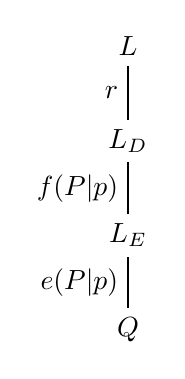
\begin{tikzpicture}[node distance = 1.2cm, auto]
      \node (Q) {$\mathbb{Q}$};
      \node (L_E) [above of=Q] {$L_E$};
      \node (L_D) [above of=L_E] {$L_D$};
      \node (L) [above of=L_D] {$L$};
      \draw[-] (Q) to node {$e(\mathfrak{P}|p)$} (L_E);
      \draw[-] (L_E) to node {$f(\mathfrak{P}|p)$} (L_D);
      \draw[-] (L_D) to node {$r$} (L);
      \end{tikzpicture}
\end{center}

where $[L:\mathbb{Q}] = 6$. From this tower of fields, we may determine the decomposition group. Let $p \in S$. For any $\mathfrak{p}$ lying over $p$, we note that $L/K$ is a Galois extension of degree $2$. Hence there are 3 possibilities for the decomposition of $\mathfrak{p}$ in $L$. Namely
\begin{enumerate}[i.]
\item $r = 2$ and  $e(\mathfrak{P}|\mathfrak{p}) = f(\mathfrak{P}|\mathfrak{p}) = 1$. Then $\mathfrak{p}\mathcal{O}_L = \mathfrak{P}_1\mathfrak{P}_2.$
\item $e(\mathfrak{P}|\mathfrak{p}) = 2$ and $r = f(\mathfrak{P}|\mathfrak{p}) = 1$. Then $\mathfrak{p}\mathcal{O}_L = \mathfrak{P}_1^2.$
\item $f(\mathfrak{P}|\mathfrak{p}) = 2$ and $r = e(\mathfrak{P}|\mathfrak{p}) = 1$. Then $\mathfrak{p}\mathcal{O}_L = \mathfrak{P}_1.$
\end{enumerate}

For $p \in S$, there are $5$ possibilities for the decomposition of $p$ in $K$. In particular,
\begin{enumerate}[1.]
\item $(p)\mathcal{O}_K = \mathfrak{p}_1$ with $e(\mathfrak{p}_1|p) = 1, f(\mathfrak{p}_1|p) = 3$. By the PIRL, it follows that this prime ideal is bounded and therefore does not appear unbounded in \eqref{Eq:TMfactored}.
\item $(p)\mathcal{O}_K = \mathfrak{p}_1^3$ with $e(\mathfrak{p}_1|p) = 3, f(\mathfrak{p}_1|p) = 1$. By the PIRL, it follows that this prime ideal is bounded and therefore does not appear unbounded in \eqref{Eq:TMfactored}.

\item $(p)\mathcal{O}_K = \mathfrak{p}_1 \mathfrak{p}_2$ with $e(\mathfrak{p}_1|p) = f(\mathfrak{p}_1|p) = 1$ and $e(\mathfrak{p}_2|p) = 1, f(\mathfrak{p}_2|p) = 2$.

Looking at the possibilities for the factorization of $\mathfrak{p}_2$ in $L$, we observe
\begin{enumerate}[i.]
\item Since 
\[e(\mathfrak{P}|p) = e(\mathfrak{P}|\mathfrak{p}_2)e(\mathfrak{p}|p) = 1 \quad \text{ and } \quad f(\mathfrak{P}|p) = f(\mathfrak{P}|\mathfrak{p}_2)f(\mathfrak{p}|p) = 2,\]
it follows from $6 = r\cdot e(\mathfrak{P}|p)\cdot f(\mathfrak{P}|p)$ that $r = 3$. Hence
\[(p)\mathcal{O}_L = \mathfrak{P}_1\mathfrak{P}_2\mathfrak{P}_3 \implies |D(\mathfrak{P}_i|p)| = 2.\]
\item Since 
\[e(\mathfrak{P}|p) = e(\mathfrak{P}|\mathfrak{p}_2)e(\mathfrak{p}|p) = 2 \quad \text{ and } \quad f(\mathfrak{P}|p) = f(\mathfrak{P}|\mathfrak{p}_2)f(\mathfrak{p}|p) = 2,\]
it follows from $6 = r\cdot e(\mathfrak{P}|p)\cdot f(\mathfrak{P}|p) = r \cdot 4$ that such a case is not possible.
\item Since 
\[e(\mathfrak{P}|p) = e(\mathfrak{P}|\mathfrak{p}_2)e(\mathfrak{p}|p) = 1 \quad \text{ and } \quad f(\mathfrak{P}|p) = f(\mathfrak{P}|\mathfrak{p}_2)f(\mathfrak{p}|p) = 4,\]
it follows from $6 = r\cdot e(\mathfrak{P}|p)\cdot f(\mathfrak{P}|p) = r \cdot 4$ that such a case is not possible.\end{enumerate}
Now, since
\[e(\mathfrak{P}|p) = 1 \quad \text{ and } \quad f(\mathfrak{P}|p) = 2\]
is the only possible case, we have that $|D(\mathfrak{P}_i|p)| = 2$ for $i = 1,2,3$.

\item $(p)\mathcal{O}_K = \mathfrak{p}_1 \mathfrak{p}_2^2$ with $e(\mathfrak{p}_1|p) = f(\mathfrak{p}_1|p) = 1$ and $e(\mathfrak{p}_2|p) = 2, f(\mathfrak{p}_2|p) = 1$.

Looking at the possibilities for the factorization of $\mathfrak{p}_2$ in $L$, we observe
\begin{enumerate}[i.]
\item Since 
\[e(\mathfrak{P}|p) = e(\mathfrak{P}|\mathfrak{p}_2)e(\mathfrak{p}|p) = 2 \quad \text{ and } \quad f(\mathfrak{P}|p) = f(\mathfrak{P}|\mathfrak{p}_2)f(\mathfrak{p}|p) = 1,\]
it follows from $6 = r\cdot e(\mathfrak{P}|p)\cdot f(\mathfrak{P}|p)$ that $r = 3$. Hence
\[(p)\mathcal{O}_L = \mathfrak{P}_1^2\mathfrak{P}_2^2\mathfrak{P}_3^2 \implies |D(\mathfrak{P}_i|p)| = 2.\]
\item Since 
\[e(\mathfrak{P}|p) = e(\mathfrak{P}|\mathfrak{p}_2)e(\mathfrak{p}|p) = 4 \quad \text{ and } \quad f(\mathfrak{P}|p) = f(\mathfrak{P}|\mathfrak{p}_2)f(\mathfrak{p}|p) = 1,\]
it follows from $6 = r\cdot e(\mathfrak{P}|p)\cdot f(\mathfrak{P}|p) = r \cdot 4$ that such a case is not possible.
\item Since 
\[e(\mathfrak{P}|p) = e(\mathfrak{P}|\mathfrak{p}_2)e(\mathfrak{p}|p) = 2 \quad \text{ and } \quad f(\mathfrak{P}|p) = f(\mathfrak{P}|\mathfrak{p}_2)f(\mathfrak{p}|p) = 2,\]
it follows from $6 = r\cdot e(\mathfrak{P}|p)\cdot f(\mathfrak{P}|p) = r \cdot 4$ that such a case is not possible.\end{enumerate}
Now, since
\[e(\mathfrak{P}|p) = 2 \quad \text{ and } \quad f(\mathfrak{P}|p) = 1\]
is the only possible case, we have that $|D(\mathfrak{P}_i|p)| = 2$ for $i = 1,2,3$.

\item $(p)\mathcal{O}_K = \mathfrak{p}_1 \mathfrak{p}_2\mathfrak{p}_3$ with $e(\mathfrak{p}_i|p) = f(\mathfrak{p}_i|p) = 1$ for $i = 1,2,3$.

Looking at the possibilities for the factorization of $\mathfrak{p}_i$ in $L$, we observe
\begin{enumerate}[i.]
\item Since 
\[e(\mathfrak{P}|p) = e(\mathfrak{P}|\mathfrak{p}_i)e(\mathfrak{p}|p) = 1 \quad \text{ and } \quad f(\mathfrak{P}|p) = f(\mathfrak{P}|\mathfrak{p}_i)f(\mathfrak{p}|p) = 1,\]
it follows from $6 = r\cdot e(\mathfrak{P}|p)\cdot f(\mathfrak{P}|p)$ that $r = 6$. Hence
\[(p)\mathcal{O}_L = \mathfrak{P}_1\mathfrak{P}_2\mathfrak{P}_3\mathfrak{P}_4\mathfrak{P}_5\mathfrak{P}_6 \implies |D(\mathfrak{P}_i|p)| = 1.\]
In this case, the only automorphism $\sigma$ on $L$ such that $\sigma(\mathfrak{P}) = \mathfrak{P}$ is the identity map, hence there can be no cancellation in this case.  
\item Since 
\[e(\mathfrak{P}|p) = e(\mathfrak{P}|\mathfrak{p}_i)e(\mathfrak{p}|p) = 2 \quad \text{ and } \quad f(\mathfrak{P}|p) = f(\mathfrak{P}|\mathfrak{p}_i)f(\mathfrak{p}|p) = 1,\]
it follows from $6 = r\cdot e(\mathfrak{P}|p)\cdot f(\mathfrak{P}|p)$ that $r = 3$. Hence
\[(p)\mathcal{O}_L = \mathfrak{P}_1^2\mathfrak{P}_2^2\mathfrak{P}_3^2 \implies |D(\mathfrak{P}_i|p)| = 2.\]
\item Since 
\[e(\mathfrak{P}|p) = e(\mathfrak{P}|\mathfrak{p}_2)e(\mathfrak{p}|p) = 1 \quad \text{ and } \quad f(\mathfrak{P}|p) = f(\mathfrak{P}|\mathfrak{p}_2)f(\mathfrak{p}|p) = 2,\]
it follows from $6 = r\cdot e(\mathfrak{P}|p)\cdot f(\mathfrak{P}|p)$ that $r = 3$. Hence
\[(p)\mathcal{O}_L = \mathfrak{P}_1\mathfrak{P}_2\mathfrak{P}_3 \implies |D(\mathfrak{P}_i|p)| = 2.\]
\end{enumerate}
\end{enumerate}

From the above list, we observe that we are left to determine whether $D(\mathfrak{P}_i|p)$ having cardinality $2$ can result in $\mathfrak{P}^{(i_0)} = \mathfrak{P}^{(j)}$. We recall that the generating automorphisms of $S_3$ either permute $\theta$ or send $\sqrt{D}$ to $-\sqrt{D}$. If we fix $\theta = \theta_1$, then, in sending $\theta_1$ to $\theta_1$, then we either select an element of $S_3$ that has order 1 (the identity map) or order $2$ ($\tau$). To send $\theta_1$ to $\theta_2$, our choices are either an order $3$ element ($\sigma$) or an order 2 element, $\tau\sigma^2$. Lastly, to send $\theta_1$ to $\theta_3$, we choose either between an order $3$ element, $\sigma^2$, or an order 2 element, $\tau\sigma$. The choice of the automorphisms themselves do not matter so long as $\theta$ is permuted. In other words, we choose $(i_0, j,k)$ so that it forms an order $3$ subgroup of $S_3$. Since only a cardinality $2$ subgroup can map a prime ideal $\mathfrak{P}$ to itself, it follows that this choice of $(i_0,j,k)$ cannot coincide with $D(\mathfrak{P}|p)$ and therefore cannot lead to $\mathfrak{P}^{(i_0)} = \mathfrak{P}^{(j)}$. 
\end{proof}

For the remainder of this paper, we assume that $(i_0,j,k)$ are automorphisms of $L$ selected as in Lemma~\ref{lem:cancellation}.

\begin{lemma}\label{lem:ordpz}
Let $\mathfrak{P}$ be a finite place of $L$ and let $\mathfrak{P}^{(i_0)} = \sigma_{i_0}(\mathfrak{P})$ and $\mathfrak{P}^{(j)} = \sigma_{j}(\mathfrak{P})$, where $\sigma_{i_0}: L \to L$, $\theta \mapsto \theta^{(i_0)}$ and $\sigma_{j}: L \to L$, $\theta \mapsto \theta^{(j)}$ are two automorphisms of $L$. For 
\[\frac{\delta_2}{\lambda}= \prod_{i = 1}^{r}\left( \frac{\varepsilon_i^{(j)}}{\varepsilon_i^{(i_0)}}\right)^{a_i} \prod_{i = 1}^{\nu} \left( \frac{\gamma_i^{(j)}}{\gamma_i^{(i_0)}}\right)^{n_i},\]
we have
\[\ord_{\mathfrak{P}}\left(\frac{\delta_2}{\lambda}\right)=
\begin{cases}
(u_l - r_l)e(\mathfrak{P}^{(j)}|\mathfrak{p}_l^{(j)})	
	& \textnormal{ if } \mathfrak{P}^{(j)} \mid p_l , \ p_l \in \{p_1,\dots, p_{\nu}\}\\
(r_l - u_l)e(\mathfrak{P}^{(i_0)}|\mathfrak{p}_l^{(i_0)})
	& \textnormal{ if } \mathfrak{P}^{(i_0)}\mid p_l, \ p_l \in \{p_1,\dots, p_{\nu}\}\\
0 	& \textnormal{ otherwise}.
\end{cases}\]
\end{lemma}
\begin{proof}

By Lemma~\ref{lem:cancellation}, we have 
\[\left( \frac{\gamma_i^{(j)}}{\gamma_i^{(i_0)}}\right)\mathcal{O}_L 
	 = \left(\prod_{\mathfrak{P}\mid\mathfrak{p}_1} \frac{\mathfrak{P}^{(j) \ e(\mathfrak{P}^{(j)}\mid\mathfrak{p}_1^{(j)})}}{\mathfrak{P}^{(i_0) \ e(\mathfrak{P}^{(i_0)}\mid\mathfrak{p}^{(i_0)}_1)}}\right)^{a_{1i}} \cdots \left(\prod_{\mathfrak{P}\mid\mathfrak{p}_{\nu}} \frac{\mathfrak{P}^{(j) \ e(\mathfrak{P}^{(j)}\mid\mathfrak{p}^{(j)}_{\nu})}}{\mathfrak{P}^{(i_0) \ e(\mathfrak{P}^{(i_0)}\mid\mathfrak{p}^{(i_0)}_{\nu})}}\right)^{a_{\nu i}}.\]
Hence
\begin{align*}
\left(\frac{\delta_2}{\lambda}\right)\mathcal{O}_L
	& = \left( \frac{\gamma_1^{(j)}}{\gamma_1^{(i_0)}}\right)^{n_1}\cdots \left( \frac{\gamma_{\nu}^{(j)}}{\gamma_{\nu}^{(i_0)}}\right)^{n_{\nu}} \mathcal{O}_L\\
	& = \left(\prod_{\mathfrak{P}\mid\mathfrak{p}_1} \frac{\mathfrak{P}^{(j) \ e(\mathfrak{P}^{(j)}\mid\mathfrak{p}_1^{(j)})}}{\mathfrak{P}^{(i_0) \ e(\mathfrak{P}^{(i_0)}\mid\mathfrak{p}^{(i_0)}_1)}}\right)^{n_1a_{11}} \cdots \left(\prod_{\mathfrak{P}\mid\mathfrak{p}_{\nu}} \frac{\mathfrak{P}^{(j) \ e(\mathfrak{P}^{(j)}\mid\mathfrak{p}^{(j)}_{\nu})}}{\mathfrak{P}^{(i_0) \ e(\mathfrak{P}^{(i_0)}\mid\mathfrak{p}^{(i_0)}_{\nu})}}\right)^{n_1a_{\nu 1}} \cdots \\
	& \quad \quad \cdots 
\left(\prod_{\mathfrak{P}\mid\mathfrak{p}_1} \frac{\mathfrak{P}^{(j) \ e(\mathfrak{P}^{(j)}\mid\mathfrak{p}_1^{(j)})}}{\mathfrak{P}^{(i_0) \ e(\mathfrak{P}^{(i_0)}\mid\mathfrak{p}^{(i_0)}_1)}}\right)^{n_{\nu}a_{1\nu}} \cdots \left(\prod_{\mathfrak{P}\mid\mathfrak{p}_{\nu}} \frac{\mathfrak{P}^{(j) \ e(\mathfrak{P}^{(j)}\mid\mathfrak{p}^{(j)}_{\nu})}}{\mathfrak{P}^{(i_0) \ e(\mathfrak{P}^{(i_0)}\mid\mathfrak{p}^{(i_0)}_{\nu})}}\right)^{n_{\nu} a_{\nu \nu}} \\
	& = \left(\prod_{\mathfrak{P}\mid\mathfrak{p}_1} \frac{\mathfrak{P}^{(j) \ e(\mathfrak{P}^{(j)}\mid\mathfrak{p}_1^{(j)})}}{\mathfrak{P}^{(i_0) \ e(\mathfrak{P}^{(i_0)}\mid\mathfrak{p}^{(i_0)}_1)}}\right)^{\sum_{i = 1}^\nu n_ia_{1i}} \cdots \left(\prod_{\mathfrak{P}\mid\mathfrak{p}_{\nu}} \frac{\mathfrak{P}^{(j) \ e(\mathfrak{P}^{(j)}\mid\mathfrak{p}^{(j)}_{\nu})}}{\mathfrak{P}^{(i_0) \ e(\mathfrak{P}^{(i_0)}\mid\mathfrak{p}^{(i_0)}_{\nu})}}\right)^{\sum_{i=1}^{\nu} n_ia_{\nu i}}\\
	& = \left(\prod_{\mathfrak{P}\mid\mathfrak{p}_1} \frac{\mathfrak{P}^{(j) \ e(\mathfrak{P}^{(j)}\mid\mathfrak{p}_1^{(j)})}}{\mathfrak{P}^{(i_0) \ e(\mathfrak{P}^{(i_0)}\mid\mathfrak{p}^{(i_0)}_1)}}\right)^{u_1 - r_1} \cdots \left(\prod_{\mathfrak{P}\mid\mathfrak{p}_{\nu}} \frac{\mathfrak{P}^{(j) \ e(\mathfrak{P}^{(j)}\mid\mathfrak{p}^{(j)}_{\nu})}}{\mathfrak{P}^{(i_0) \ e(\mathfrak{P}^{(i_0)}\mid\mathfrak{p}^{(i_0)}_{\nu})}}\right)^{u_{\nu} - r_{\nu}}\\
\end{align*}
and so
\[\ord_{\mathfrak{P}}\left( \frac{\delta_2}{\lambda}\right)=
\begin{cases}
(u_l - r_l)e(\mathfrak{P}^{(j)}|\mathfrak{p}_l^{(j)})	
	& \textnormal{ if } \mathfrak{P}^{(j)} \mid p_l , \ p_l \in \{p_1,\dots, p_{\nu}\}\\
(r_l - u_l)e(\mathfrak{P}^{(i_0)}|\mathfrak{p}_l^{(i_0)})
	& \textnormal{ if } \mathfrak{P}^{(i_0)}\mid p_l, \ p_l \in \{p_1,\dots, p_{\nu}\}\\
0 	& \textnormal{ otherwise}.
\end{cases}\]
\end{proof}

Let $\log^+(\cdot)$ denote the real valued function $\max(\log(\cdot), 0)$ on $\mathbb{R}_{\geq 0}$. 

\begin{proposition}\label{prop:heightdecomp}
The height $h\left(\frac{\delta_2}{\lambda}\right)$ admits a decomposition
\[h\left(\frac{\delta_2}{\lambda}\right) = \frac{1}{[K:\mathbb{Q}]}\sum_{l = 1}^{\nu} \log(p_l)|u_l - r_l| + \frac{1}{[L:\mathbb{Q}]}\sum_{w :L \to \mathbb{C}} \log \max \left\{ \left|w\left(\frac{\delta_2}{\lambda}\right)\right|, 1\right\} \]

Further, if $\deg{g(t)}=3$ then 
\[\sum_{w :L \to \mathbb{C}} \log \max \left\{ \left|w\left(\frac{\delta_2}{\lambda}\right)\right|, 1\right\} = 
\begin{cases}
2\max_{w:L\to \mathbb{C}} \log \max \left\{ \left|w\left(\frac{\delta_2}{\lambda}\right)\right|, 1\right\} & \text{ if } \sqrt{\Delta}\notin\mathbb{Q} \\
\max_{w:L\to \mathbb{C}}\sum_{w :L \to \mathbb{C}} \log \max \left\{ \left|w\left(\frac{\delta_2}{\lambda}\right)\right|, 1\right\} & \text{ if } \sqrt{\Delta}\in\mathbb{Q} \\
\end{cases}\]
when one can choose $(i_0),(j), (k) : L \to \mathbb{C}$ such that $\mathfrak{p}_{p}^{(j)} \neq \mathfrak{p}_{p}^{(i_0)}$ for all $p \in S$. 
\end{proposition}

\begin{proof}[Proof of Proposition~\ref{prop:heightdecomp}]Since $\frac{\delta_2}{\lambda} \in L$, the definition of the absolute logarithmic Weil height gives
\[h\left(\frac{\delta_2}{\lambda}\right)=\frac{1}{[L:\mathbb{Q}]}\sum_{w \in M_L} \log \max \left\{ \left\|\frac{\delta_2}{\lambda}\right\|_{w}, 1\right\}\]
where $||z||_w$ are the usual norms and $M_L$ is a set of inequivalent absolute values on $L$. 

In particular, if $w: L \to \mathbb{C}$ is an infinite place, we obtain
\[ \log \max \left\{ \left\|\frac{\delta_2}{\lambda}\right\|_{w}, 1\right\} = \log \max \left\{ \left|w\left(\frac{\delta_2}{\lambda}\right)\right|, 1\right\}.\]

Now, for $z = \frac{\delta_2}{\lambda}$ and $w = \mathfrak{P}$ a finite place, we have
\[ \log \max \{ \|z\|_{w}, 1\} = \max \left\{ \log\left(\frac{1}{N(\mathfrak{P})^{\ord_{\mathfrak{P}}(z)}} \right), 0\right\}. \]
By Lemma~\ref{lem:ordpz}, 
\[\ord_{\mathfrak{P}}\left( \frac{\delta_2}{\lambda}\right)=
\begin{cases}
(u_l - r_l)e(\mathfrak{P}^{(j)}|\mathfrak{p}_l^{(j)})	
	& \textnormal{ if } \mathfrak{P}^{(j)} \mid p_l , \ p_l \in \{p_1,\dots, p_{\nu}\}\\
(r_l - u_l)e(\mathfrak{P}^{(i_0)}|\mathfrak{p}_l^{(i_0)})
	& \textnormal{ if } \mathfrak{P}^{(i_0)}\mid p_l, \ p_l \in \{p_1,\dots, p_{\nu}\}\\
0 	& \textnormal{ otherwise}.
\end{cases}\]
That is, for $\mathfrak{P}^{(j)}\mid p_l$ where $p_l \in \{p_1, \dots, p_{\nu}\}$, we have
\begin{align*}
 \log \max \{ ||z||_{w}, 1\}	
 	& = \max \left\{ \log\left(\frac{1}{N(\mathfrak{P})^{\ord_{\mathfrak{P}}(z)}} \right), 0\right\}\\
	& = \max \left\{ \log\left(\frac{1}{N(\mathfrak{P})^{(u_l - r_l)e(\mathfrak{P}^{(j)}|\mathfrak{p}_l^{(j)})}} \right), 0\right\}\\
	& = \max \left\{ \log\left(\frac{1}{p_l^{(u_l - r_l)f(\mathfrak{P}^{(j)}\mid p_l)e(\mathfrak{P}^{(j)}|\mathfrak{p}_l^{(j)})}} \right), 0\right\}\\
	& = \max \left\{ -(u_l - r_l)f(\mathfrak{P}^{(j)}\mid p_l)e(\mathfrak{P}^{(j)}|\mathfrak{p}_l^{(j)})\log(p_l), 0\right\}.
\end{align*}
For $p_l \in \{p_1, \dots, p_{\nu}\}$, there is 1 unique prime ideal $\mathfrak{p}_1$ in the ideal equation \eqref{Eq:TMfactored} lying above $p_l$ in $K$. Hence, each $\mathfrak{P}$ lying over $p_l$ must also lie over $\mathfrak{p}_l$. Now, 
\begin{align*}
\sum_{\mathfrak{P}^{(j)} \mid \mathfrak{p}_l^{(j)}} \log \max \left\{ \left\|\frac{\delta_2}{\lambda}\right\|_{w}, 1\right\}
	& = \sum_{\mathfrak{P}^{(j)} \mid \mathfrak{p}_l^{(j)}} \max \left\{ -(u_l - r_l)f(\mathfrak{P}^{(j)}\mid p_l)e(\mathfrak{P}^{(j)}|\mathfrak{p}_l^{(j)})\log(p_l), 0\right\}\\
	& = \max \left\{ (r_l - u_l)\log(p_l), 0\right\}\sum_{\mathfrak{P}^{(j)} \mid \mathfrak{p}_l^{(j)}}f(\mathfrak{P}^{(j)}\mid p_l)e(\mathfrak{P}^{(j)}|\mathfrak{p}_l^{(j)})\\
	& = \max \left\{ (r_l - u_l)\log(p_l), 0\right\}\sum_{\mathfrak{P}^{(j)} \mid \mathfrak{p}_l^{(j)}}f(\mathfrak{P}^{(j)}\mid \mathfrak{p}_l^{(j)})f(\mathfrak{p}_l^{(j)}\mid p_l)e(\mathfrak{P}^{(j)}|\mathfrak{p}_l^{(j)})\\
	& = \max \left\{ (r_l - u_l)\log(p_l), 0\right\}f(\mathfrak{p}_l^{(j)}\mid p_l)\sum_{\mathfrak{P}^{(j)} \mid \mathfrak{p}_l^{(j)}}f(\mathfrak{P}^{(j)}\mid \mathfrak{p}_l^{(j)})e(\mathfrak{P}^{(j)}|\mathfrak{p}_l^{(j)})\\
	& = \max \left\{ (r_l - u_l)\log(p_l), 0\right\}f(\mathfrak{p}_l^{(j)}\mid p_l)[L:\mathbb{Q}(\theta^{(j)})]\\
	& = \max \left\{ (r_l - u_l)\log(p_l), 0\right\}f(\mathfrak{p}_l^{(j)}\mid p_l)[L:K].
\end{align*}
where the last inequality follows from $K = \mathbb{Q}(\theta) \cong \mathbb{Q}(\theta^{(j)})$

Similarly, for $\mathfrak{P}^{(i_0)}\mid p_l$ where $p_l \in \{p_1, \dots, p_{\nu}\}$, we have
\begin{align*}
 \log \max \{ \|z\|_{w}, 1\}	
 	& = \max \left\{ \log\left(\frac{1}{N(\mathfrak{P})^{\ord_{\mathfrak{P}}(z)}} \right), 0\right\}\\
	& = \max \left\{ \log\left(\frac{1}{N(\mathfrak{P})^{(r_l - u_l)e(\mathfrak{P}^{(i_0)}|\mathfrak{p}_l^{(i_0)})}} \right), 0\right\}\\
	& = \max \left\{ \log\left(\frac{1}{p_l^{(r_l - u_l)f(\mathfrak{P}^{(i_0)}\mid p_l)e(\mathfrak{P}^{(i_0)}|\mathfrak{p}_l^{(i_0)})}} \right), 0\right\}\\
	& = \max \left\{ -(r_l - u_l)f(\mathfrak{P}^{(i_0)}\mid p_l)e(\mathfrak{P}^{(i_0)}|\mathfrak{p}_l^{(i_0)})\log(p_l), 0\right\},
\end{align*}
and so
\begin{align*}
\sum_{\mathfrak{P}^{(i_0)} \mid \mathfrak{p}_l^{(i_0)}} \log \max \left\{ \left\|\frac{\delta_2}{\lambda}\right\|_{w}, 1\right\}
	& = \max \left\{ (u_l - r_l)\log(p_l), 0\right\}f(\mathfrak{p}_l^{(i_0)}\mid p_l)[L:K].
\end{align*}

Lastly, if $w = \mathfrak{P}$ such that $\mathfrak{P} \neq \mathfrak{P}^{(i_0)},  \mathfrak{P}^{(j)}$, we have
\begin{align*}
 \log \max \{ \|z\|_{w}, 1\}	
 	& = \max \left\{ \log\left(\frac{1}{N(\mathfrak{P})^{\ord_{\mathfrak{P}}(z)}} \right), 0\right\}\\
	& = \max \left\{ \log\left(\frac{1}{N(\mathfrak{P})^{0}} \right), 0\right\}\\
	& = 0.
\end{align*}

Now, we have 
\begin{align*}
h\left(\frac{\delta_2}{\lambda}\right)
	& =\frac{1}{[L:\mathbb{Q}]}\sum_{w \in M_L} \log \max \left\{ \left\|\frac{\delta_2}{\lambda}\right\|_{w}, 1\right\}\\
	& = \frac{1}{[L:\mathbb{Q}]}\sum_{w :L \to \mathbb{C}} \log \max \left\{ \left|w\left(\frac{\delta_2}{\lambda}\right)\right|, 1\right\} + \frac{1}{[L:\mathbb{Q}]}\sum_{\mathfrak{P} \in \mathcal{O}_L \text{ finite }} \log \max \left\{ \left\|\frac{\delta_2}{\lambda}\right\|_{\mathfrak{P}}, 1\right\},
\end{align*}
where
\begin{align*}
& \sum_{\mathfrak{P} \in \mathcal{O}_L \text{ finite }} \log \max \left\{ \left\|\frac{\delta_2}{\lambda}\right\|_{w}, 1\right\} \\
	& = \sum_{l = 1}^{\nu} \left(\sum_{\mathfrak{P}^{(j)} \mid \mathfrak{p}_l^{(j)}} \log \max \left\{ \left\|\frac{\delta_2}{\lambda}\right\|_{w}, 1\right\} + \sum_{\mathfrak{P}^{(i_0)} \mid \mathfrak{p}_l^{(i_0)}} \log \max \left\{ \left\|\frac{\delta_2}{\lambda}\right\|_{w}, 1\right\}\right)\\
	& = \sum_{l = 1}^{\nu} \left(\max \left\{ (r_l - u_l)\log(p_l), 0\right\}f(\mathfrak{p}_l^{(j)}\mid p_l)[L:K] + \max \left\{ (u_l - r_l)\log(p_l), 0\right\}f(\mathfrak{p}_l^{(i_0)}\mid p_l)[L:K]\right)\\
	& =  [L:K]\sum_{l = 1}^{\nu} \log(p_l)\left(\max \left\{ -(u_l - r_l), 0\right\}+ \max \left\{ (u_l - r_l), 0\right\}\right)\\
	& =  [L:K]\sum_{l = 1}^{\nu} \log(p_l)\max \left\{ -(u_l - r_l), (u_l - r_l)\right\}\\
	& =  [L:K]\sum_{l = 1}^{\nu} \log(p_l)|u_l - r_l|.
\end{align*}
Here, we recall that $K = \mathbb{Q}(\theta) \cong \mathbb{Q}(\theta^{(i_0)}) \cong \mathbb{Q}(\theta^{(j)})$ and therefore 
\[f(\mathfrak{p}_l^{(i_0)}\mid p_l) = f(\mathfrak{p}_l^{(j)}\mid p_l) = f(\mathfrak{p}_l\mid p_l) = 1.\]
Altogether, we have
\begin{align*}
h\left(\frac{\delta_2}{\lambda}\right)
	& =\frac{1}{[L:\mathbb{Q}]}\sum_{w \in M_L} \log \max \left\{ \left\|\frac{\delta_2}{\lambda}\right\|_{w}, 1\right\}\\
	& = \frac{1}{[L:\mathbb{Q}]}\sum_{w :L \to \mathbb{C}} \log \max \left\{ \left|w\left(\frac{\delta_2}{\lambda}\right)\right|, 1\right\} + \frac{1}{[L:\mathbb{Q}]}\sum_{\mathfrak{P} \in \mathcal{O}_L \text{ finite }} \log \max \left\{ \left\|\frac{\delta_2}{\lambda}\right\|_{\mathfrak{P}}, 1\right\}\\
	& = \frac{1}{[L:\mathbb{Q}]}\sum_{w :L \to \mathbb{C}} \log \max \left\{ \left|w\left(\frac{\delta_2}{\lambda}\right)\right|, 1\right\} + \frac{1}{[K:\mathbb{Q}]}\sum_{l = 1}^{\nu} \log(p_l)|u_l - r_l|\\
	& = \frac{1}{[L:\mathbb{Q}]}\sum_{w :L \to \mathbb{C}} \log \max \left\{ \left|w\left(\frac{\delta_2}{\lambda}\right)\right|, 1\right\} + \frac{1}{[K:\mathbb{Q}]}\log\left(p_1^{|u_1 - r_1|} \cdots p_{\nu}^{|u_{\nu} - r_{\nu}|}\right)
\end{align*}

To prove the last statement, we first assume that $\sqrt{\Delta}\in\mathbb{Q}$. Then $L=\mathbb{Q}(\theta, \sqrt{\Delta}) = \mathbb{Q}(\theta) = K$ and the Galois group of $L/\mathbb{Q}$ is the alternating group $A_3$. Hence the Galois group is generated by $\sigma$, which takes $\theta$ to one of the other roots of $g(t)$. In particular, 
\[\Gal(L/\mathbb{Q}) = \{ \text{id}_\text{L}, \sigma, \sigma^2\},\]
where
\begin{align*}
\text{id}_{\text{L}}: 
\begin{cases}
\theta_1 \mapsto \theta_1\\
\theta_2 \mapsto \theta_2\\
\theta_3 \mapsto \theta_3\\
\sqrt{D} \mapsto \sqrt{D}
\end{cases}
& \quad ,
\sigma: 
\begin{cases}
\theta_1 \mapsto \theta_2\\
\theta_2 \mapsto \theta_3\\
\theta_3 \mapsto \theta_1\\
\sqrt{D} \mapsto \sqrt{D}
\end{cases}
& \quad ,
\sigma^2: 
\begin{cases}
\theta_1 \mapsto \theta_3\\
\theta_2 \mapsto \theta_1\\
\theta_3 \mapsto \theta_2\\
\sqrt{D} \mapsto \sqrt{D}
\end{cases},
\end{align*}
Writing $j = 1, i_0 = 2$ and $k = 3$, the orbit of 
\[\frac{\delta_2}{\lambda}= \prod_{i = 1}^{r}\left( \frac{\varepsilon_i^{(1)}}{\varepsilon_i^{(2)}}\right)^{a_i} \prod_{i = 1}^{\nu} \left( \frac{\gamma_i^{(1)}}{\gamma_i^{(2)}}\right)^{n_i}\in L\]
is
\[\left\{ \prod_{i = 1}^{r}\left( \frac{\varepsilon_i^{(1)}}{\varepsilon_i^{(2)}}\right)^{a_i} \prod_{i = 1}^{\nu} \left( \frac{\gamma_i^{(1)}}{\gamma_i^{(2)}}\right)^{n_i}, 
	\prod_{i = 1}^{r}\left( \frac{\varepsilon_i^{(2)}}{\varepsilon_i^{(3)}}\right)^{a_i} \prod_{i = 1}^{\nu} \left( \frac{\gamma_i^{(2)}}{\gamma_i^{(3)}}\right)^{n_i}, 
	\prod_{i = 1}^{r}\left( \frac{\varepsilon_i^{(3)}}{\varepsilon_i^{(1)}}\right)^{a_i} \prod_{i = 1}^{\nu} \left( \frac{\gamma_i^{(3)}}{\gamma_i^{(1)}}\right)^{n_i}\right\}.\]
We choose $a,b,c\in\{1,2,3\}$ such that 
\[ \left|\prod_{i = 1}^{r}\left( \varepsilon_i^{(a)}\right)^{a_i} \prod_{i = 1}^{\nu} \left( \gamma_i^{(a)}\right)^{n_i}\right| \geq
	\left|\prod_{i = 1}^{r}\left( \varepsilon_i^{(b)}\right)^{a_i} \prod_{i = 1}^{\nu} \left( \gamma_i^{(b)}\right)^{n_i}\right| \geq
	\left|\prod_{i = 1}^{r}\left( \varepsilon_i^{(c)}\right)^{a_i} \prod_{i = 1}^{\nu} \left( \gamma_i^{(c)}\right)^{n_i}\right|.\]
Then we obtain
\begin{align*}
\sum_{w :L \to \mathbb{C}} \log \max \left\{ \left|w\left(\frac{\delta_2}{\lambda}\right)\right|, 1\right\}
	& = \log \max \left\{ \left|\text{id}_L\left(\frac{\delta_2}{\lambda}\right)\right|, 1\right\} 
		+ \log \max \left\{ \left|\sigma\left(\frac{\delta_2}{\lambda}\right)\right|,1\right\} \\
		& \quad+ \log \max \left\{ \left|\sigma^2\left(\frac{\delta_2}{\lambda}\right)\right|, 1\right\}\\
	& = \log \max \left\{ \left|\prod_{i = 1}^{r}\left( \frac{\varepsilon_i^{(a)}}{\varepsilon_i^{(b)}}\right)^{a_i} \prod_{i = 1}^{\nu} \left( \frac{\gamma_i^{(a)}}{\gamma_i^{(b)}}\right)^{n_i} \right|, 1\right\} \\
		& \quad + \log \max \left\{ \left|\ \prod_{i = 1}^{r}\left( \frac{\varepsilon_i^{(b)}}{\varepsilon_i^{(c)}}\right)^{a_i} \prod_{i = 1}^{\nu} \left( \frac{\gamma_i^{(b)}}{\gamma_i^{(c)}}\right)^{n_i} \right|,1\right\} \\
		& \quad+ \log \max \left\{ \left| \prod_{i = 1}^{r}\left( \frac{\varepsilon_i^{(c)}}{\varepsilon_i^{(a)}}\right)^{a_i} \prod_{i = 1}^{\nu} \left( \frac{\gamma_i^{(c)}}{\gamma_i^{(a)}}\right)^{n_i} \right|, 1\right\}\\
	& = \log  \left|\prod_{i = 1}^{r}\left( \frac{\varepsilon_i^{(a)}}{\varepsilon_i^{(b)}}\right)^{a_i} \prod_{i = 1}^{\nu} \left( \frac{\gamma_i^{(a)}}{\gamma_i^{(b)}}\right)^{n_i} \right| \\
		& \quad + \log \left|\ \prod_{i = 1}^{r}\left( \frac{\varepsilon_i^{(b)}}{\varepsilon_i^{(c)}}\right)^{a_i} \prod_{i = 1}^{\nu} \left( \frac{\gamma_i^{(b)}}{\gamma_i^{(c)}}\right)^{n_i} \right| \\
	& = \log  \left|\prod_{i = 1}^{r}\left( \frac{\varepsilon_i^{(a)}}{\varepsilon_i^{(c)}}\right)^{a_i} \prod_{i = 1}^{\nu} \left( \frac{\gamma_i^{(a)}}{\gamma_i^{(c)}}\right)^{n_i} \right|.
\end{align*}
Hence it follows that
\[\sum_{w :L \to \mathbb{C}} \log \max \left\{ \left|w\left(\frac{\delta_2}{\lambda}\right)\right|, 1\right\} = 
\max_{w:L\to \mathbb{C}}\sum_{w :L \to \mathbb{C}} \log \max \left\{ \left|w\left(\frac{\delta_2}{\lambda}\right)\right|, 1\right\}.\]

It remains to consider the case when $\sqrt{\Delta} \notin \mathbb{Q}$. Then the Galois group of $L/\mathbb{Q}$ is the symmetric group $S_3$. We now write $j = 1, i_0 = 2,$ and $k = 3$, the orbit of 
\[\frac{\delta_2}{\lambda}= \prod_{i = 1}^{r}\left( \frac{\varepsilon_i^{(1)}}{\varepsilon_i^{(2)}}\right)^{a_i} \prod_{i = 1}^{\nu} \left( \frac{\gamma_i^{(1)}}{\gamma_i^{(2)}}\right)^{n_i}\in L\]
is
\begin{align*}
& \left\{ \prod_{i = 1}^{r}\left( \frac{\varepsilon_i^{(1)}}{\varepsilon_i^{(2)}}\right)^{a_i} \prod_{i = 1}^{\nu} \left( \frac{\gamma_i^{(1)}}{\gamma_i^{(2)}}\right)^{n_i} , 
	\prod_{i = 1}^{r}\left( \frac{\varepsilon_i^{(2)}}{\varepsilon_i^{(3)}}\right)^{a_i} \prod_{i = 1}^{\nu} \left( \frac{\gamma_i^{(2)}}{\gamma_i^{(3)}}\right)^{n_i}, 
	\prod_{i = 1}^{r}\left( \frac{\varepsilon_i^{(3)}}{\varepsilon_i^{(1)}}\right)^{a_i} \prod_{i = 1}^{\nu} \left( \frac{\gamma_i^{(3)}}{\gamma_i^{(1)}}\right)^{n_i} \right. \\
	& \quad \left. \prod_{i = 1}^{r}\left( \frac{\varepsilon_i^{(3)}}{\varepsilon_i^{(2)}}\right)^{a_i} \prod_{i = 1}^{\nu} \left( \frac{\gamma_i^{(3)}}{\gamma_i^{(2)}}\right)^{n_i} , 
	\prod_{i = 1}^{r}\left( \frac{\varepsilon_i^{(1)}}{\varepsilon_i^{(3)}}\right)^{a_i} \prod_{i = 1}^{\nu} \left( \frac{\gamma_i^{(1)}}{\gamma_i^{(3)}}\right)^{n_i}, 
	\prod_{i = 1}^{r}\left( \frac{\varepsilon_i^{(2)}}{\varepsilon_i^{(1)}}\right)^{a_i} \prod_{i = 1}^{\nu} \left( \frac{\gamma_i^{(2)}}{\gamma_i^{(1)}}\right)^{n_i} \right\}.
\end{align*}
We choose $a,b,c\in\{1,2,3\}$ such that 
\[ \left|\prod_{i = 1}^{r}\left( \varepsilon_i^{(a)}\right)^{a_i} \prod_{i = 1}^{\nu} \left( \gamma_i^{(a)}\right)^{n_i}\right| \geq
	\left|\prod_{i = 1}^{r}\left( \varepsilon_i^{(b)}\right)^{a_i} \prod_{i = 1}^{\nu} \left( \gamma_i^{(b)}\right)^{n_i}\right| \geq
	\left|\prod_{i = 1}^{r}\left( \varepsilon_i^{(c)}\right)^{a_i} \prod_{i = 1}^{\nu} \left( \gamma_i^{(c)}\right)^{n_i}\right|.\]
Then we obtain
\begin{align*}
\sum_{w :L \to \mathbb{C}} \log \max \left\{ \left|w\left(\frac{\delta_2}{\lambda}\right)\right|, 1\right\}
	& = \log \max \left\{ \left|\text{id}_L\left(\frac{\delta_2}{\lambda}\right)\right|, 1\right\} 
		+ \log \max \left\{ \left|\sigma\left(\frac{\delta_2}{\lambda}\right)\right|,1\right\} \\
		& \quad+ \log \max \left\{ \left|\sigma^2\left(\frac{\delta_2}{\lambda}\right)\right|, 1\right\} + \log \max \left\{ \left|\tau\left(\frac{\delta_2}{\lambda}\right)\right|, 1\right\}\\
		& \quad+ \log \max \left\{ \left|\tau\sigma\left(\frac{\delta_2}{\lambda}\right)\right|, 1\right\} + \log \max \left\{ \left|\tau\sigma^2\left(\frac{\delta_2}{\lambda}\right)\right|, 1\right\}\\
	& = \log \left|\prod_{i = 1}^{r}\left( \frac{\varepsilon_i^{(a)}}{\varepsilon_i^{(b)}}\right)^{a_i} \prod_{i = 1}^{\nu} \left( \frac{\gamma_i^{(a)}}{\gamma_i^{(b)}}\right)^{n_i} \right|\\
		& \quad + \log \left|\ \prod_{i = 1}^{r}\left( \frac{\varepsilon_i^{(b)}}{\varepsilon_i^{(c)}}\right)^{a_i} \prod_{i = 1}^{\nu} \left( \frac{\gamma_i^{(b)}}{\gamma_i^{(c)}}\right)^{n_i} \right|\\
		& \quad+ \log \left| \prod_{i = 1}^{r}\left( \frac{\varepsilon_i^{(a)}}{\varepsilon_i^{(c)}}\right)^{a_i} \prod_{i = 1}^{\nu} \left( \frac{\gamma_i^{(a)}}{\gamma_i^{(c)}}\right)^{n_i} \right|\\
	& = 2\log  \left|\prod_{i = 1}^{r}\left( \frac{\varepsilon_i^{(a)}}{\varepsilon_i^{(c)}}\right)^{a_i} \prod_{i = 1}^{\nu} \left( \frac{\gamma_i^{(a)}}{\gamma_i^{(c)}}\right)^{n_i} \right|.
\end{align*}
Hence it follows that
\[\sum_{w :L \to \mathbb{C}} \log \max \left\{ \left|w\left(\frac{\delta_2}{\lambda}\right)\right|, 1\right\} = 
2\max_{w:L\to \mathbb{C}}\sum_{w :L \to \mathbb{C}} \log \max \left\{ \left|w\left(\frac{\delta_2}{\lambda}\right)\right|, 1\right\}.\]
\end{proof}

%---------------------------------------------------------------------------------------------------------------------------------------------%
\subsection{Initial height bounds}

Recall that we seek solutions to
\begin{equation*}
\lambda = \delta_1 \prod_{i = 1}^r\left( \frac{\varepsilon_i^{(k)}}{\varepsilon_i^{(j)}}\right)^{a_i}\prod_{i = 1}^{\nu} \left( \frac{\gamma_i^{(k)}}{\gamma_i^{(j)}}\right)^{n_i} - 1 = \delta_2 \prod_{i = 1}^{r}\left( \frac{\varepsilon_i^{(i_0)}}{\varepsilon_i^{(j)}}\right)^{a_i} \prod_{i = 1}^{\nu} \left( \frac{\gamma_i^{(i_0)}}{\gamma_i^{(j)}}\right)^{n_i},
\end{equation*}
where
\[\delta_1 = \frac{\theta^{(i_0)} - \theta^{(j)}}{\theta^{(i_0)} - \theta^{(k)}}\cdot\frac{\alpha^{(k)}\zeta^{(k)}}{\alpha^{(j)}\zeta^{(j)}}, \quad \delta_2 = \frac{\theta^{(j)} - \theta^{(k)}}{\theta^{(k)} - \theta^{(i_0)}}\cdot \frac{\alpha^{(i_0)}\zeta^{(i_0)}}{\alpha^{(j)}\zeta^{(j)}}\]
are constants and $r = 1$ or $r = 2$. 

In Rafael's notation, let
\[y =  \prod_{i = 1}^r\left( \frac{\varepsilon_i^{(k)}}{\varepsilon_i^{(j)}}\right)^{a_i}\prod_{i = 1}^{\nu} \left( \frac{\gamma_i^{(k)}}{\gamma_i^{(j)}}\right)^{n_i}, \quad 
x = \prod_{i = 1}^{r}\left( \frac{\varepsilon_i^{(i_0)}}{\varepsilon_i^{(j)}}\right)^{a_i} \prod_{i = 1}^{\nu} \left( \frac{\gamma_i^{(i_0)}}{\gamma_i^{(j)}}\right)^{n_i}\]
so that our equation is
\[\delta_1y - 1 = \delta_2x.\]
Equivalently, letting $\mu_0 = \delta_1$ and $\lambda_0 = \delta_2$, we arrive at
\[\mu_0y - \lambda_0x = 1,\]
just as in Rafael's notation. 

Returning to our notation, we see that 
\begin{align*}
\lambda 	& = \delta_2 \prod_{i = 1}^{r}\left( \frac{\varepsilon_i^{(i_0)}}{\varepsilon_i^{(j)}}\right)^{a_i} \prod_{i = 1}^{\nu} \left( \frac{\gamma_i^{(i_0)}}{\gamma_i^{(j)}}\right)^{n_i}\\
		& = \delta_2 x\\
		& = \lambda_0 x.
\end{align*}
Hence, let $z:= \frac{1}{x} = \frac{\delta_2}{\lambda}$.

Now, let $\Sigma$ denote the set of pairs $(x,y)$ satisfying the equation 
\[\mu_0y - \lambda_0x = 1.\]
That is, let $\Sigma$ denote the set of tuples $(n_1, \dots, n_{\nu}, a_1, \dots, a_r)$ giving $x,y$ which satisfy
\[\mu_0y - \lambda_0x = 1.\]

Let $l,h\in\mathbb{R}^{S^*}$ with $0\leq l\leq h$. Then we define $\Sigma(l,h)$ as the set of all $(x,y)\in \Sigma$ such that $\left(h_v\left(\frac{\delta_2}{\lambda}\right)\right)\leq h$ and such that $\left(h_v\left(\frac{\delta_2}{\lambda}\right)\right)\nleq l$, 
\[\Sigma(l,h) = \{(x,y) \in \Sigma \ | \ (h_v(z))\leq h \text{ and } (h_v(z))\nleq l\}.\]
Since we are comparing vectors, we note that $(h_v(z))\nleq l$ does not necessarily mean that $l < (h_v(z))$. Instead, this means that not \textit{all} coordinates $h_v(z)$ satisfy $h_v(z) \leq l_v$, and hence there is at least one coordinate for which $h_v(z) > l_v$.

Here we write $\Sigma(h)=\Sigma(l,h)$ if $l=0$.  
\[\Sigma(h) = \Sigma(0,h)= \{(x,y) \in \Sigma \ | \ (h_v(z))\leq h \text{ and }  (h_v(z))\nleq 0 \},\]
so that at least one coordinate satisfies $h_v(z) > 0$.

Further, for each $w\in S^*$, we denote by $\Sigma_w(l,h)$ the set of all $(x,y)\in\Sigma(h)$ such that $h_w(z)>l_w$. 
\begin{align*}
\Sigma_w(l,h)	& = \{(x,y) \in \Sigma(h) \ | \ h_w(z)>l_w \} \\
			& = \{(x,y) \in \Sigma \ | \ (h_v(z))\leq h \text{ and }  (h_v(z))\nleq 0 \text{ and } h_w(z)>l_w\}.
\end{align*}

Recall that 
\[f(X,Y) = X^3 + C_1 X^{2}Y + C_2XY^2 + C_3Y^3 = c p_1^{z_1} \cdots p_v^{z_v}.\]
and $\gcd(X,Y)=1$ and $S = \{p_1, \dots, p_v\}$. Let 
\[N_S = \prod_{p\in S}p.\]
To measure an integer $m$ and the finite set $S$, we take
\begin{align*}
m_S	& = 1728 N_S^2 \prod_{p \notin S} p^{\min(2,\ord_p(m))}\\
	& = 1728 \prod_{p\in S}p^2 \prod_{\substack{p \notin S \\ p \mid m}} p^{\min(2,\ord_p(m))}.
\end{align*}
Recall further that the Weil height of an integer $n \in \mathbb{Z}\backslash {0}$ is given by
\[h(n) = \log|n|.\] 
Now, denote by $h(f-c)$ the maximum logarithmic Weil heights of the coefficients of the polynomial $f - c$,
\begin{align*}
h(f-a)	& = h(x^3 + C_1 x^{2}y + C_2xy^2 + C_3y^3 - c)\\
		& = \max(h(1), h(C_1), h(C_2), h(C_3), h(-c))\\
		& = \max(\log|1|, \log|C_1|, \log|C_2|, \log|C_3|, \log|c|)\\
		& = \max(0, \log|C_1|, \log|C_2|, \log|C_3|, \log|c|)\\
		& = \max(\log|C_1|, \log|C_2|, \log|C_3|, \log|c|),		
\end{align*}
where we recall that $C_i \in \mathbb{N}$.
Put $m = 432 \Delta c^2$ with $\Delta$ the discriminant of $F$. Now, let 
\[\Omega = 2m_S \log(m_S) + 172h(f-c).\]
By Rafael and Benjamin's paper, 
\[\max(h(X),h(Y))\leq \Omega. \]

We recall that  
\[\beta = X-Y\theta = \alpha \zeta \varepsilon_1^{a_1} \cdots \varepsilon_r^{a_r}\cdot \gamma_1^{n_1}\cdots \gamma_{\nu}^{n_{\nu}}\]
and we define
\[\Omega' = 2h(\alpha) + 4\Omega + 2h(\theta) + 2\log(2).\]

For $z \in K$, we recall
\[h(z)=\frac{1}{[K:\mathbb{Q}]}\sum_{w \in M_K} \log \max \left\{ \left\|z\right\|_{w}, 1\right\}\]
where $||z||_w$ are the usual norms and $M_K$ is a set of inequivalent absolute values on $K$. Now, 
\[(\alpha)\mathcal{O}_K = \mathfrak{p}_1^{A_1} \cdots \mathfrak{p}_n^{A_n} \quad \text{ and } \quad (\theta)\mathcal{O}_K = \mathfrak{p}_1^{B_1} \cdots \mathfrak{p}_m^{B_m}.\]
For $w = \mathfrak{p}$ a finite place, we have
\[ \log \max \{ \|z\|_{w}, 1\} = \max \left\{ \log\left(\frac{1}{N(\mathfrak{p}_i)^{\ord_{\mathfrak{p}_i}(\alpha)}} \right), 0\right\} = \max \left\{ \log\left(\frac{1}{p^{fA_i}} \right), 0\right\} = 0\]
and 
\[ \log \max \{ \|z\|_{w}, 1\} = \max \left\{ \log\left(\frac{1}{N(\mathfrak{p}_i)^{\ord_{\mathfrak{p}_i}(\theta)}} \right), 0\right\} = \max \left\{ \log\left(\frac{1}{p^{fB_i}} \right), 0\right\} = 0.\]
It follows that
\[h(\alpha)=\frac{1}{[K:\mathbb{Q}]}\sum_{w \in M_K} \log \max \left\{ \left\|\alpha\right\|_{w}, 1\right\}
	= \frac{1}{[K:\mathbb{Q}]}\sum_{\sigma:K \to \mathbb{C}} \log \max \left\{ |\sigma(\alpha)|, 1\right\}
\]
and 
\[h(\theta)=\frac{1}{[K:\mathbb{Q}]}\sum_{w \in M_K} \log \max \left\{ \left\|\theta\right\|_{w}, 1\right\}
	= \frac{1}{[K:\mathbb{Q}]}\sum_{\sigma:K \to \mathbb{C}} \log \max \left\{ |\sigma(\theta)|, 1\right\}.
\]
Now, 
\begin{align*}
\Omega'	
	& = 2h(\alpha) + 4\Omega + 2h(\theta) + 2\log(2)\\
	& = \frac{2}{[K:\mathbb{Q}]}\sum_{\sigma:K \to \mathbb{C}} \log \max \left\{ |\sigma(\alpha)|, 1\right\} + 4\Omega + \frac{2}{[K:\mathbb{Q}]}\sum_{\sigma:K \to \mathbb{C}} \log \max \left\{ |\sigma(\theta)|, 1\right\} + 2\log(2)
\end{align*}

\begin{lemma}
Let ${\mathbf{m} = (n_1, \dots, n_{\nu}, a_1, \dots, a_r) \in \mathbb{R}^{r + \nu}}$ be any solution of \eqref{Eq:main3}. If $\mathbf{h} \in\mathbb{R}^{\nu + r}$ with $\mathbf{h} = (\Omega')$, then $\mathbf{m}\in \Sigma(h)$, where
\[\Sigma(h) = \Sigma(0,h)= \{(x,y) \in \Sigma \ | \ (h_v(z))\leq h \text{ and }  (h_v(z))\nleq 0 \},\]
\end{lemma}
That is, all solutions $(x,y) \in \Sigma$ satisfy $\mathbf{m}\in \Sigma(h)$ if $\mathbf{h} = (\Omega')$.

\begin{proof}
Let $(x,y) \in \Sigma$. Then $(x,y)$ satisfy $\mu_0y-\lambda_0x=1$. We must show that the resulting value of $z:= \frac{1}{x} = \frac{\delta_2}{\lambda}$ arising from this choice of $x,y$ satisfies
\[0 < \left(h_v\left(\frac{\delta_2}{\lambda}\right)\right)\leq h.\]
Now, via Rafael and Benjamin, for a solution $X,Y$ of $f(X,Y) = c p_1^{z_1}\cdots p_v^{z_v}$, we have
\[\max(h(X),h(Y)) \leq \Omega.\]
We use the following height properties
\begin{enumerate}
\item For a non-zero rational number $a/b$ where $\gcd(a,b) = 1$,
\[h(a/b) = \max \{\log{|a|}, \log{|b|}\}\]
\item For $\alpha \in \overline{\mathbb{Q}}$, $n \in \mathbb{N}$, we have
\[h(n \alpha) = n h(\alpha).\]
\item For $\alpha, \beta \in \overline{\mathbb{Q}}$, we have
\[h(\alpha + \beta) \leq h(\alpha) + h(\beta) + \log{2}.\]
\item For $\alpha, \beta \in \overline{\mathbb{Q}}$, we have
\[h(\alpha\beta) \leq h(\alpha) + h(\beta).\]
\item For $\alpha \in \overline{\mathbb{Q}}$, we have
\[h(1/\alpha) = h(\alpha).\]
\end{enumerate}

Now, applying these properties to $\beta = X-\theta Y$, we obtain
\begin{align*}
h(\beta)	& = h(X-\theta Y)\\
		& \leq h(X) + h(-\theta Y) + \log{2}\\
		& \leq h(X) + h(-\theta) + h(Y) + \log{2}\\
		& = h(X) + h(\theta) + h(Y) + \log{2}\\
		& \leq 2\Omega + h(\theta) + \log{2}.
\end{align*}
Now, $h(\beta) = h(\beta^{(i)})$, hence
\[h(\beta^{(i)}) \leq 2\Omega + h(\theta) + \log{2}.\]
Further, we have
\begin{align*}
\delta_2x	& =  \delta_2 \prod_{i = 1}^{r}\left( \frac{\varepsilon_i^{(i_0)}}{\varepsilon_i^{(j)}}\right)^{a_i} \prod_{i = 1}^{\nu} \left( \frac{\gamma_i^{(i_0)}}{\gamma_i^{(j)}}\right)^{n_i} \\
		& =  \frac{\theta^{(j)} - \theta^{(k)}}{\theta^{(k)} - \theta^{(i_0)}}\cdot \frac{\alpha^{(i_0)}\zeta^{(i_0)}}{\alpha^{(j)}\zeta^{(j)}} \prod_{i = 1}^{r}\left( \frac{\varepsilon_i^{(i_0)}}{\varepsilon_i^{(j)}}\right)^{a_i} \prod_{i = 1}^{\nu} \left( \frac{\gamma_i^{(i_0)}}{\gamma_i^{(j)}}\right)^{n_i} \\
		& = \frac{\theta^{(j)} - \theta^{(k)}}{\theta^{(k)} - \theta^{(i_0)}}\cdot \frac{\beta^{(i_0)}}{\beta^{(j)}}.
\end{align*}
This means that 
\begin{align*}
x	& = \frac{\theta^{(j)} - \theta^{(k)}}{\theta^{(k)} - \theta^{(i_0)}}\cdot \frac{\beta^{(i_0)}}{\beta^{(j)}}\cdot\frac{1}{\delta_2}\\
	& =  \frac{\theta^{(j)} - \theta^{(k)}}{\theta^{(k)} - \theta^{(i_0)}}\cdot \frac{\beta^{(i_0)}}{\beta^{(j)}}\cdot\frac{1}{\frac{\theta^{(j)} - \theta^{(k)}}{\theta^{(k)} - \theta^{(i_0)}}\cdot \frac{\alpha^{(i_0)}\zeta^{(i_0)}}{\alpha^{(j)}\zeta^{(j)}}}\\
	& = \frac{\theta^{(j)} - \theta^{(k)}}{\theta^{(k)} - \theta^{(i_0)}}\cdot \frac{\beta^{(i_0)}}{\beta^{(j)}}\cdot\frac{\theta^{(k)} - \theta^{(i_0)}}{\theta^{(j)} - \theta^{(k)}}\cdot \frac{\alpha^{(j)}\zeta^{(j)}}{\alpha^{(i_0)}\zeta^{(i_0)}}\\
	& =\frac{\beta^{(i_0)}}{\beta^{(j)}}\cdot \frac{\alpha^{(j)}\zeta^{(j)}}{\alpha^{(i_0)}\zeta^{(i_0)}}.
\end{align*}
Hence, 
\begin{align*}
h(x)	& = h\left( \frac{\beta^{(i_0)}}{\beta^{(j)}}\cdot \frac{\alpha^{(j)}\zeta^{(j)}}{\alpha^{(i_0)}\zeta^{(i_0)}}\right)\\
	& = h(\beta^{(i_0)}) + h\left( \frac{1}{\beta^{(j)}}\right) + h(\alpha^{(j)}) + h\left( \frac{1}{\alpha^{(i_0)}}\right)+ h(\zeta^{(j)}) + h\left( \frac{1}{\zeta^{(i_0)}}\right)\\
	& = 2h(\beta) + 2h(\alpha) + 2h(\zeta)\\
	& \leq 2(2\Omega + h(\theta) + \log{2}) +2h(\alpha) + 2h(\zeta)\\
	& = 4\Omega + 2h(\theta) + 2\log{2} + 2h(\alpha) + 2h(\zeta).
\end{align*}
Now, 
\begin{align*}
h(\zeta)	& =\frac{1}{[K:\mathbb{Q}]}\sum_{w \in M_K} \log \max \left\{ \left\|\zeta\right\|_{w}, 1\right\}\\
		& = \frac{1}{[K:\mathbb{Q}]}\sum_{\sigma:K \to \mathbb{C}} \log \max \left\{ |\sigma(\zeta)|, 1\right\}\\
		& = \frac{1}{[K:\mathbb{Q}]}\sum_{\sigma:K \to \mathbb{C}} \log \max \left\{ 1, 1\right\}\\
		& = 0.
\end{align*}
Therefore, 
\[h(x) \leq 4\Omega + 2h(\theta) + 2\log{2} + 2h(\alpha) = \Omega'\]
and hence
\[h(z) = h\left(\frac{\delta_2}{\lambda}\right) = h(1/x) = h(x) \leq \Omega'.\]
Together with $\displaystyle h_v\left(\frac{\delta_2}{\lambda}\right) \leq h\left(\frac{\delta_2}{\lambda}\right)$ implies
\[h_v\left(\frac{\delta_2}{\lambda}\right) \leq \Omega'\]
for each $v \in S^*.$
Similarly, by definition, we have $h_v\left(\frac{\delta_2}{\lambda}\right) \geq 0$. That is, $(x,y) \in \Sigma(h)$ as required. 
\end{proof}

\subsection{Coverings of $\Sigma$}

From the previous section, we see that all solutions $(x,y) \in \Sigma$ satisfy $\mathbf{m}\in \Sigma(h)$ if ${\mathbf{h} = (\Omega')}$.

Now, let $l,h\in\mathbb{R}^{\nu+r}$ with $0\leq l\leq h$. With the definitions of the previous section, we have that

\begin{lemma}\label{lem:covering}
It holds that $\Sigma(h)=\Sigma(l,h)\cup \Sigma(l)$ and $\Sigma(l,h)=\cup_{v\in S^*}\Sigma_v(l,h)$.
\end{lemma}
\begin{proof}
Recall that 
\[\Sigma(l,h) = \{(x,y) \in \Sigma \ | \ (h_v(z))\leq h \text{ and } (h_v(z))\nleq l\},\]
\[\Sigma(h) = \Sigma(0,h)= \{(x,y) \in \Sigma \ | \ (h_v(z))\leq h \text{ and }  (h_v(z))\nleq 0 \},\]
and for each $w\in S^*$
\[\Sigma_w(l,h) = \{(x,y) \in \Sigma \ | \ (h_v(z))\leq h \text{ and }  (h_v(z))\nleq 0 \text{ and } h_w(z)>l_w\}.\]

Suppose $(x,y) \in \Sigma(h)$. By definition this means, $(h_v(z))\leq h$ and that $h_v(z) > 0$ for at least one coordinate. Since $0 \leq l \leq h$, it follows that either $(h_v(z))\leq l$ or $(h_v(z))\nleq l$. That is, either all coordinates satisfy $h_v(z) \leq l_v$, or there is at least one coordinate for which $h_v(z) > l_v$, meaning that either $(x,y) \in \Sigma(l)$ or $(x,y) \in \Sigma(l,h)$. Hence $(x,y) \in \Sigma(l,h) \cup \Sigma(l)$. That is, $\Sigma(h) \subseteq \Sigma(l,h) \cup \Sigma(l)$.

Conversely, we suppose that $(x,y) \in \Sigma(l,h) \cup \Sigma(l)$. It follows that either $(h_v(z))\leq h \text{ and } (h_v(z))\nleq l$ or $(h_v(z))\leq l \text{ and } (h_v(z))\nleq 0$. In either case, this means that $(h_v(z)) \leq h$ and $(h_v(z)) \nleq 0$. Hence $(x,y) \in \Sigma(h)$. Thus $\Sigma(h) \supseteq \Sigma(l,h) \cup \Sigma(l)$. Together with the previous paragraph, this yields $\Sigma(h)=\Sigma(l,h)\cup \Sigma(l)$.

To prove the second point, let $(x,y) \in \Sigma(l,h)$. Then there exists $w\in S^*$ with $h_w(z)>l_w$ and thus $(x,y)$ lies in $\Sigma_w(l,h)$. Hence $\Sigma(l,h) \subseteq \cup_{v\in S^*}\Sigma_v(l,h)$. Lastly, since each set $\Sigma_v(l,h)$ is contained in $\Sigma(l,h)$ it follows that $\Sigma(l,h)=\cup_{v\in S^*}\Sigma_v(l,h)$.
\end{proof}

Suppose now we are given an initial bound $h_0$ with $\Sigma=\Sigma(h_0)$ and pairs $(l_n,h_n)\in \mathbb{R}^{\nu + r}\times \mathbb{R}^{\nu + r}$ with $0\leq l_n\leq h_n$ and $h_{n+1}=l_{n}$ for $n=0,\dotsc,N$. Then we can cover $\Sigma$: $$\Sigma=\Sigma(l_{N})\cup\bigl(\cup_{n=0}^{N}\cup_{v\in S^*}\Sigma_v(l_n,h_n)\bigl).$$
Indeed this follows directly by applying the above lemma $N$ times. In the subsequent sections, we shall show that one can efficiently enumerate each set $\Sigma_v(l_n,h_n)$ by finding all points in the intersection $\Gamma_v\cap \mathcal E_v$ of a lattice $\Gamma_v$ with an ellipsoid $\mathcal E_v$.





If $h_0=(b,\dotsc,b)$ for $b$ the initial height bound, then
Lemma~\ref{lem:covering} gives  $$\Sigma=\Sigma(h_0), \quad \Sigma(h)=\Sigma(l,h)\cup \Sigma(l) \quad \textnormal{and} \quad \Sigma(l,h)=\cup_{v\in S^*}\Sigma_v(l,h).$$
Thus, after choosing a good sequence of lower and upper bounds (i.e. $l,h\in R^{S^*}$ with $0\leq l\leq h$) covering the whole space $0\leq h_0$, we are reduced to compute $\Sigma_v(l,h)$.
%
%
\subsubsection{Refined coverings}
%
%Next, for any nonempty subset $V\subseteq S^*$ we denote by $\Sigma_V(l,v)$ the set of all $(x,y)\in \Sigma(l,h)$ such that $h_v(z)>l_v$ for each $v\in V$ and such that $h_v(z)\leq l_v$ for each $v\in S^*\setminus V$.
%
%
%\begin{lemma}[Refined coverings]
%It holds that $\Sigma(l,h)
%=\cup_{V}\Sigma_V(l,h)$ with the union taken over all nonempty subsets $V\subseteq S^*$.
%\end{lemma}
%\begin{proof}
%To see that $\Sigma(l,h)\subseteq \cup_V\Sigma_V(l,h)$, we take $(x,y)$ in $\cup_V\Sigma_V(l,h)$ and we let $V$ be the set of $v\in S^*$ with $h_v(z)>l_v$. Then the set $V$ is nonempty since $(h_v(z))\nleq l$ and thus $(x,y)$ lies in $\Sigma_V(l,h)$. This proves that $\Sigma(l,h)= \cup_V\Sigma_V(l,h)$.
%\end{proof}
%Suppose again we are given an initial bound $h_0$ with $\Sigma=\Sigma(h_0)$ and pairs $(l_n,h_n)\in \RR^{S^*}\times \RR^{S^*}$ with $0\leq l_n\leq h_n$ and $h_{n+1}=l_{n}$ for $n=0,\dotsc,N$. Then we can cover $\Sigma$: $$\Sigma=\Sigma(l_{N})\cup\bigl(\cup_{n=0}^{N}\cup_{V\subseteq S^*}\Sigma_V(l_n,h_n)\bigl).$$
%Indeed this follows directly by applying the above lemma $N$ times. In the subsequent sections, we shall show that one can efficiently enumerate each set $\Sigma_V(l_n,h_n)$ by finding all points in the intersection $\Gamma_V\cap \mathcal E_V$ of a lattice $\Gamma_V=\cap_{v\in V}\Gamma_v$ with an ellipsoid $\mathcal E_V$.
%
%Note these refined coverings are not that efficient in practice. We should consider the refined coverings from the elllog sieve.
%

%---------------------------------------------------------------------------------------------------------------------------------------------%
\subsection{Controlling the exponents in terms of the Weil Height}

We now work with the norm $\|\cdot \|_\infty$. However, below we shall give much more precise estimates (which are essentially optimal) to make the volumes of the involved ellipsoids as small as possible. 

\subsubsection{Bounding $\{n_1, \dots, n_{\nu}\}$}
\begin{lemma}
For any solution $(x,y, a_1, \dots, a_r, n_1, \dots, n_{\nu})$ of \eqref{Eq:main3}, we have 
\[\|\mathbf{n}\|_{\infty} \leq \|A^{-1}\|_{\infty} \frac{h\left(\frac{\delta_2}{\lambda}\right)}{\log(2)}.\]
\end{lemma}

\begin{proof}
Recall that $\mathbf{n} = (n_1, \dots, n_{\nu})^{\text{T}}$ and 
\[A\mathbf{n} = \mathbf{u} - \mathbf{r}.\]
Now, taking the $\| \cdot \|_{\infty}$ norm of both sides yields
\[ \mathbf{n} = A^{-1}( \mathbf{u} - \mathbf{r} ) \implies \|\mathbf{n}\|_{\infty} = \|A^{-1} (\mathbf{u} - \mathbf{r})\|_{\infty} \leq \|A^{-1}\|_{\infty} \|\mathbf{u} - \mathbf{r}\|_{\infty}.\]
Here, 
\[\|\mathbf{u}-\mathbf{r}\|_{\infty} = \max_{1 \leq l \leq \nu} |u_l - r_l|.\]
Now, since
\[h\left(\frac{\delta_2}{\lambda}\right) = \frac{1}{[L:\mathbb{Q}]}\sum_{w :L \to \mathbb{C}} \log \max \left\{ \left|w\left(\frac{\delta_2}{\lambda}\right)\right|, 1\right\} + \frac{1}{[K:\mathbb{Q}]}\sum_{l = 1}^{\nu} \log(p_l)|u_l - r_l|,\]
it follows that 
\[0 \leq |u_l - r_l| \log(p_l) \leq h\left(\frac{\delta_2}{\lambda}\right)\]
for each $l \in \{1, \dots, \nu\}$. In other words, 
\[|u_l - r_l| \leq \frac{h\left(\frac{\delta_2}{\lambda}\right)}{\log(p_l)}\]
and so
\[\max_{1 \leq l \leq \nu} |u_l - r_l| \leq \max_{1\leq l\leq \nu}\left(\frac{h\left(\frac{\delta_2}{\lambda}\right)}{\log(p_l)}\right) = \frac{h\left(\frac{\delta_2}{\lambda}\right)}{\log(2)}.\]
Altogether this gives
\[\|\mathbf{n}\|_{\infty} \leq \|A^{-1}\|_{\infty} \|\mathbf{u} - \mathbf{r}\|_{\infty} \leq \|A^{-1}\|_{\infty} \frac{h\left(\frac{\delta_2}{\lambda}\right)}{\log(2)}.\]
\end{proof}

\subsubsection{Bounding $\{a_1, \dots, a_{r}\}$}

We next consider the quadratic form $q_f=A^TD^2A$ on $\mathbb{Z}^{\nu}$ and where $D^2$ is a $\nu \times \nu$ diagonal matrix with diagonal entries $\lfloor\frac{\log(p_i)^2}{\log(2)^2}\rfloor$ for $p_i \in S$. We note that $\lfloor(\log(2))^2\rfloor = 0$, so if the diagonal entries of $D$ were set to $\lfloor\log(p_i)^2$ and $2\in S$, our matrix $D$ would not be invertible. In this case, when generating the lattice and ellipsoid, this will yield a matrix which is not positive-definite, meaning that we will not be able to apply Fincke-Pohst. With this in mind, the quadratic form $q_f$ is positive definite since $A$ is invertible. 

\begin{lemma}
For any solution $(x,y, n_1, \dots, n_{\nu}, a_1, \dots, a_r)$ of \eqref{Eq:main3}, we have 
\[\frac{\log(2)^2}{[K:\mathbb{Q}]}q_f(\mathbf{n}) = \frac{\log(2)^2}{[K:\mathbb{Q}]}\sum_{l = 1}^{\nu} \left\lfloor\frac{\log(p_l)^2}{\log(2)^2}\right\rfloor|u_l -r_l|^2 < \left(h\left(\frac{\delta_2}{\lambda}\right)\right)^2.\] 
\end{lemma}

\begin{proof}
Recall that $\mathbf{n} = (n_1, \dots, n_{\nu})^{\text{T}}$ and 
\[A\mathbf{n} = \mathbf{u} - \mathbf{r}.\]
Assume first that $2 \notin S$. Now
\begin{align*}
q_f(\mathbf{n})	
	& = (A\mathbf{n})^{\text{T}}D^2A\mathbf{n}\\
	& = \mathbf{n}^{\text{T}}A^{\text{T}}D^2A\mathbf{n}\\
	& = (\mathbf{u} - \mathbf{r})^{\text{T}}D^2(\mathbf{u} - \mathbf{r})\\
	& = \begin{pmatrix} u_1 - r_1&  \dots & u_{\nu} - r_{\nu} \end{pmatrix} 
		\begin{pmatrix} \lfloor\frac{\log(p_1)^2}{\log(2)^2}\rfloor& 0 & \dots & 0\\ 0 &\lfloor\frac{\log(p_2)^2}{\log(2)^2}\rfloor & \dots & 0\\
		\vdots & \vdots & \ddots & \vdots\\ 0 & 0 & \dots & \lfloor\frac{\log(p_{\nu})^2}{\log(2)^2}\rfloor\\ 
		\end{pmatrix} 
		\begin{pmatrix} u_1 - r_1 \\  \vdots \\ u_{\nu} - r_{\nu} \end{pmatrix} \\
	& =\left\lfloor\frac{\log(p_1)^2}{\log(2)^2}\right\rfloor(u_1-r_1)^2 + \cdots + \left\lfloor\frac{\log(p_{\nu})^2}{\log(2)^2}\right\rfloor(u_{\nu}-r_{\nu})^2\\
	& = \sum_{l = 1}^{\nu}\left\lfloor\frac{\log(p_l)^2}{\log(2)^2}\right\rfloor|u_l-r_l|^2.
\end{align*}
Hence it follows that
\[ q_f(\mathbf{n}) = \sum_{l = 1}^{\nu}\left\lfloor\frac{\log(p_l)^2}{\log(2)^2}\right\rfloor|u_l-r_l|^2.\]
Now, recall that
\[h\left(\frac{\delta_2}{\lambda}\right) = \frac{1}{[K:\mathbb{Q}]}\sum_{l = 1}^{\nu} \log(p_l)|u_l - r_l| + \frac{1}{[L:\mathbb{Q}]}\sum_{w :L \to \mathbb{C}} \log \max \left\{ \left|w\left(\frac{\delta_2}{\lambda}\right)\right|, 1\right\}.\]
It follows that
\begin{align*}
\frac{\log(2)^2}{[K:\mathbb{Q}]}q_f(\mathbf{n}) 
	& = \frac{\log(2)^2}{[K:\mathbb{Q}]}\sum_{l = 1}^{\nu} \left\lfloor\frac{\log(p_l)^2}{\log(2)^2}\right\rfloor|u_l -r_l|^2 \\
	& \leq \frac{\log(2)^2}{[K:\mathbb{Q}]}\sum_{l = 1}^{\nu}\frac{\log(p_l)^2}{\log(2)^2}|u_l -r_l|^2 \\
	& = \frac{1}{[K:\mathbb{Q}]}\sum_{l = 1}^{\nu}\log(p_l)^2|u_l -r_l|^2 \\
%	& < \frac{1}{[L:\mathbb{Q}]}\sum_{w :L \to \mathbb{C}} \left(\log \max \left\{ \left|w\left(\frac{\delta_2}{\lambda}\right)\right|, 1\right\}\right)^2 + \frac{1}{[K:\mathbb{Q}]}\sum_{l = 1}^{\nu} \left(\log(p_l)|u_l - r_l|\right)^2\\
%	& < \left(h\left(\frac{\delta_2}{\lambda}\right)\right)^2 
\end{align*}
since all terms are positive. 

If $2 \in S$, we have
\begin{align*}
q_f(\mathbf{n})	
	& = (A\mathbf{n})^{\text{T}}D^2A\mathbf{n}\\
	& = \mathbf{n}^{\text{T}}A^{\text{T}}D^2A\mathbf{n}\\
	& = (\mathbf{u} - \mathbf{r})^{\text{T}}D^2(\mathbf{u} - \mathbf{r})\\
	& = \begin{pmatrix} u_1 - r_1&  \dots & u_{\nu} - r_{\nu} \end{pmatrix} 
		\begin{pmatrix} \lfloor\frac{\log(2)^2}{\log(2)^2}\rfloor& 0 & \dots & 0\\ 0 &\lfloor\frac{\log(p_2)^2}{\log(2)^2}\rfloor & \dots & 0\\
		\vdots & \vdots & \ddots & \vdots\\ 0 & 0 & \dots & \lfloor\frac{\log(p_{\nu})^2}{\log(2)^2}\rfloor\\ 
		\end{pmatrix} 
		\begin{pmatrix} u_1 - r_1 \\  \vdots \\ u_{\nu} - r_{\nu} \end{pmatrix} \\
	& = \begin{pmatrix} u_1 - r_1&  \dots & u_{\nu} - r_{\nu} \end{pmatrix} 
		\begin{pmatrix} 1 & 0 & \dots & 0\\ 0 &\lfloor\frac{\log(p_2)^2}{\log(2)^2}\rfloor & \dots & 0\\
		\vdots & \vdots & \ddots & \vdots\\ 0 & 0 & \dots & \lfloor\frac{\log(p_{\nu})^2}{\log(2)^2}\rfloor\\ 
		\end{pmatrix} 
		\begin{pmatrix} u_1 - r_1 \\  \vdots \\ u_{\nu} - r_{\nu} \end{pmatrix} \\
	& = (u_1-r_1)^2  + \left\lfloor\frac{\log(p_2)^2}{\log(2)^2}\right\rfloor(u_2-r_2)^2 + \cdots + \left\lfloor\frac{\log(p_{\nu})^2}{\log(2)^2}\right\rfloor(u_{\nu}-r_{\nu})^2\\
	& = |u_1 - r_1|^2 + \sum_{l = 2}^{\nu}\left\lfloor\frac{\log(p_l)^2}{\log(2)^2}\right\rfloor|u_l-r_l|^2.
\end{align*}
Hence it follows that
\[ q_f(\mathbf{n}) = |u_1 - r_1|^2 + \sum_{l = 2}^{\nu}\left\lfloor\frac{\log(p_l)^2}{\log(2)^2}\right\rfloor|u_l-r_l|^2.\]
Now, recall that
\[h\left(\frac{\delta_2}{\lambda}\right) = \frac{1}{[K:\mathbb{Q}]}\sum_{l = 1}^{\nu} \log(p_l)|u_l - r_l| + \frac{1}{[L:\mathbb{Q}]}\sum_{w :L \to \mathbb{C}} \log \max \left\{ \left|w\left(\frac{\delta_2}{\lambda}\right)\right|, 1\right\}.\]
It follows that
\begin{align*}
\frac{\log(2)^2}{[K:\mathbb{Q}]}q_f(\mathbf{n}) 
	& = \frac{\log(2)^2}{[K:\mathbb{Q}]}\left( |u_1 - r_1|^2 + \sum_{l = 2}^{\nu} \left\lfloor\frac{\log(p_l)^2}{\log(2)^2}\right\rfloor|u_l -r_l|^2\right) \\
	& \leq \frac{\log(2)^2}{[K:\mathbb{Q}]}\left( |u_1 - r_1|^2 + \sum_{l = 2}^{\nu} \frac{\log(p_l)^2}{\log(2)^2}|u_l -r_l|^2\right) \\
	& = \frac{1}{[K:\mathbb{Q}]}\left( \log(2)^2|u_1 - r_1|^2 + \sum_{l = 2}^{\nu} \log(p_l)^2|u_l -r_l|^2\right) \\
	& = \frac{1}{[K:\mathbb{Q}]}\sum_{l = 1}^{\nu}\log(p_l)^2|u_l -r_l|^2
\end{align*}
since all terms are positive. 
\end{proof}

Now, 
\[\frac{\log(2)^2}{[K:\mathbb{Q}]}q_f(\mathbf{n}) =  \frac{\log(2)^2}{[K:\mathbb{Q}]} \sum_{l = 1}^{\nu}\left\lfloor\frac{\log(p_l)^2}{\log(2)^2}\right\rfloor|u_l-r_l|^2.\]

Take $\mathbf{h}\in\mathbb{R}^{r+\nu}$ such that $\mathbf{h}\geq \mathbf{0}$. Let $\mathbf{m} = (n_1, \dots, n_{\nu}, a_1, \dots, a_r) \in \mathbb{R}^{r + \nu}$ be any solution of \eqref{Eq:main3}. Denote by $h_{v}\left(\frac{\delta_2}{\lambda}\right)$ the $v^{\text{th}}$ entry of the solution vector
\[\left(\log(p_1)|u_1 - r_1|, \dots, \log(p_{\nu})|u_{\nu} - r_{\nu}|, \log \max \left\{ \left|w_1\left(\frac{\delta_2}{\lambda}\right)\right|, 1\right\}, \dots, \log \max \left\{ \left|w_n\left(\frac{\delta_2}{\lambda}\right)\right|, 1\right\}  \right)\] 
and suppose $h_v(z)\leq h_v$ for all $v\in \{1, \dots, r+\nu\}$. Then we deduce
\[\log(2)^2q_f(\mathbf{n}) = \log(2)^2\sum_{k = 1}^{\nu}\left\lfloor\frac{\log(p_k)^2}{\log(2)^2}\right\rfloor|u_k-r_k|^2 \leq \sum_{k = 1}^{\nu} \log(p_k)^2|u_k -r_k|^2 \leq \sum_{k = 1}^{\nu} h_k^2.\]

Recall that for the degree $3$ Thue-Mahler equation, either $r = 1$ or $r = 2$. Choose a set $I$ of embeddings $L \rightarrow \mathbb{C}$ of cardinality $r$. For $r = 1$, this is simply
\[R = \begin{pmatrix}
	\log\left|\left(\frac{\varepsilon_1^{(j)}}{\varepsilon_1^{(i_0)}}\right)^{\iota_1}\right| \end{pmatrix}.\]
Clearly, as long as we choose $\iota_1$ such that $\log\left|\left(\frac{\varepsilon_1^{(j)}}{\varepsilon_1^{(i_0)}}\right)^{\iota_1}\right| \neq 0$, that is $\left|\left(\frac{\varepsilon_1^{(j)}}{\varepsilon_1^{(i_0)}}\right)^{\iota_1}\right| \neq 1$, this matrix is invertible, with inverse matrix
\[R^{-1} = \begin{pmatrix} \frac{1}{\log\left|\left(\frac{\varepsilon_1^{(j)}}{\varepsilon_1^{(i_0)}}\right)^{\iota_1}\right|}\end{pmatrix}.\]

When $r = 2$, we let $I$ be the set of embeddings $L \to \mathbb{C}$ of cardinality $2$ such that for any $\alpha \in K$, it holds that $I\alpha^{(i_0)} \cup I\alpha^{(j)} = \Gal(L/\mathbb{Q})\alpha$. Such a set $I$ exists. Then we consider the $2 \times 2$ matrix
\[R = \begin{pmatrix}
	\log\left|\left(\frac{\varepsilon_1^{(j)}}{\varepsilon_1^{(i_0)}}\right)^{\iota_1}\right| &
	\log\left|\left(\frac{\varepsilon_2^{(j)}}{\varepsilon_2^{(i_0)}}\right)^{\iota_1}\right|\\
	\log\left|\left(\frac{\varepsilon_1^{(j)}}{\varepsilon_1^{(i_0)}}\right)^{\iota_2}\right| &
	\log\left|\left(\frac{\varepsilon_2^{(j)}}{\varepsilon_2^{(i_0)}}\right)^{\iota_2}\right|\\
	\end{pmatrix}.\]
Here, we let $I$ be the set of embeddings $L \to \mathbb{C}$ of cardinality $2$ such that for any $\alpha \in K$, it holds that $I\alpha^{(i_0)} \cup I\alpha^{(j)} = \Gal(L/\mathbb{Q})\alpha$. Such a set $I$ exists. 
\begin{lemma}
When $r = 2$, the matrix $R$ has an inverse
\[R^{-1} = \begin{pmatrix}
	\overline{r}_{11} & \overline{r}_{12} \\
	\overline{r}_{21} & \overline{r}_{22}
\end{pmatrix}.\]
\end{lemma}
	
\begin{proof}
See Rafael's proof.
\end{proof}

\textbf{Bounding $\{a_1, \dots, a_r\}$ when $r = 1$.}\\

Suppose first that $r = 1$. Now, for any solution $(x,y, a_1, n_1, \dots, n_{\nu})$ of \eqref{Eq:main3}, set
\[\vec{\varepsilon} = \begin{pmatrix} a_1 \end{pmatrix}.\]
Now, 
\begin{align*}
R\vec{\varepsilon}
	& = \begin{pmatrix}
		\log\left|\left(\frac{\varepsilon_1^{(j)}}{\varepsilon_1^{(i_0)}}\right)^{\iota_1}\right| \end{pmatrix}
		\begin{pmatrix} a_1\end{pmatrix}\\
	& = \begin{pmatrix} 
		a_1\log\left|\left(\frac{\varepsilon_1^{(j)}}{\varepsilon_1^{(i_0)}}\right)^{\iota_1}\right| \end{pmatrix}\\
	& = \begin{pmatrix} 
		\log\left|\left(\frac{\varepsilon_1^{(j)}}{\varepsilon_1^{(i_0)}}\right)^{\iota_1}\right|^{a_1} 	 		\end{pmatrix}\\
	& = \begin{pmatrix} 
		\log\left|\left(\frac{\varepsilon_1^{(j)}}{\varepsilon_1^{(i_0)}}\right)^{\iota_1 \ a_1}\right| 		 \end{pmatrix}.
\end{align*}
Since $R$ is invertible, we find
\begin{align*}
\vec{\varepsilon} = \begin{pmatrix} a_1\end{pmatrix} 
& =  R^{-1} \begin{pmatrix} \log\left|\left(\frac{\varepsilon_1^{(j)}}{\varepsilon_1^{(i_0)}}\right)^{\iota_1 \ 		a_1}\right| \end{pmatrix}\\
& = \begin{pmatrix} \frac{1}{\log\left|\left(\frac{\varepsilon_1^{(j)}}{\varepsilon_1^{(i_0)}}\right)^{\iota_1}\right|}	\end{pmatrix}
	\begin{pmatrix} \log\left|\left(\frac{\varepsilon_1^{(j)}}{\varepsilon_1^{(i_0)}}\right)^{\iota_1 \ a_1}\right| 	\end{pmatrix}\\
& = \begin{pmatrix} \overline{r}_{11} \end{pmatrix}\begin{pmatrix} \log\left|\left(\frac{\varepsilon_1^{(j)}}		{\varepsilon_1^{(i_0)}}\right)^{\iota_1 \ a_1}\right| \end{pmatrix}\\
& = \begin{pmatrix} \overline{r}_{11}\log\left|\left(\frac{\varepsilon_1^{(j)}}{\varepsilon_1^{(i_0)}}\right)^{\iota_1 \ 	a_1}\right|\end{pmatrix}.
\end{align*}

It follows that 
\[a_1 =  \overline{r}_{11}\log\left|\left(\frac{\varepsilon_1^{(j)}}{\varepsilon_1^{(i_0)}}\right)^{\iota_1 \ 	a_1}\right|.\]

Now, to estimate $|a_1|$, we begin to estimate the sum on the right hand side. For this, we consider
\[\frac{\delta_2}{\lambda}= \left( \frac{\varepsilon_1^{(j)}}{\varepsilon_1^{(i_0)}}\right)^{a_1}\prod_{i = 1}^{\nu} \left( \frac{\gamma_i^{(j)}}{\gamma_i^{(i_0)}}\right)^{n_i}.\]
For any embedding $\iota: L \to \mathbb{C}$, we have 
\[\left(\frac{\delta_2}{\lambda}\right)^{\iota} \prod_{i = 1}^{\nu} \left( \frac{\gamma_i^{(i_0)}}{\gamma_i^{(j)}}\right)^{\iota \ n_i} =  \left( \frac{\varepsilon_1^{(j)}}{\varepsilon_1^{(i_0)}}\right)^{\iota \ a_1}.\] 

Taking absolute values, we obtain
\[\left|\left(\frac{\delta_2}{\lambda}\right)^{\iota} \prod_{i = 1}^{\nu} \left( \frac{\gamma_i^{(i_0)}}{\gamma_i^{(j)}}\right)^{\iota \ n_i}\right| = \left|\left( \frac{\varepsilon_1^{(j)}}{\varepsilon_1^{(i_0)}}\right)^{\iota \ a_1}\right|,\]
so that
\begin{align*}
\log\left|\left( \frac{\varepsilon_1^{(j)}}{\varepsilon_1^{(i_0)}}\right)^{\iota \ a_1}\right|
	& = \log\left|\left(\frac{\delta_2}{\lambda}\right)^{\iota} \prod_{i = 1}^{\nu} \left( \frac{\gamma_i^{(i_0)}}{\gamma_i^{(j)}}\right)^{\iota \ n_i}\right|\\
	& = \log\left|\left(\frac{\delta_2}{\lambda}\right)^{\iota}\right| + \log\left| \prod_{i = 1}^{\nu} \left( \frac{\gamma_i^{(i_0)}}{\gamma_i^{(j)}}\right)^{\iota \ n_i}\right|\\
	& = \log\left|\left(\frac{\delta_2}{\lambda}\right)^{\iota}\right| - \log\left| \prod_{i = 1}^{\nu} \left( \frac{\gamma_i^{(j)}}{\gamma_i^{(i_0)}}\right)^{\iota \ n_i}\right|. 
\end{align*}

Hence, 
\begin{align*}
a_1	& =  \overline{r}_{11}\log\left|\left(\frac{\varepsilon_1^{(j)}}{\varepsilon_1^{(i_0)}}\right)^{\iota_1 \ 	a_1}\right| \\
	& = \overline{r}_{11}\left( \log\left|\left(\frac{\delta_2}{\lambda}\right)^{\iota_1}\right| - \log\left| \prod_{i = 1}^{\nu} \left( \frac{\gamma_i^{(j)}}{\gamma_i^{(i_0)}}\right)^{\iota_1 \ n_i}\right|\right)\\
	& = \overline{r}_{11}\left(\log\left|\left(\frac{\delta_2}{\lambda}\right)^{\iota_1}\right| - 
	n_1\log\left| \left( \frac{\gamma_1^{(j)}}{\gamma_1^{(i_0)}}\right)^{\iota_1}\right| - \cdots -n_{\nu}\log \left|\left( \frac{\gamma_{\nu}^{(j)}}{\gamma_{\nu}^{(i_0)}}\right)^{\iota_1}\right|\right).
\end{align*}

Recall that 
\[A\mathbf{n} = \mathbf{u} - \mathbf{r}\]
so
\[\mathbf{n} = A^{-1}(\mathbf{u} - \mathbf{r}).\]
If 
\[A = \begin{pmatrix}
	a_{11} & a_{12} & \dots & a_{1\nu} \\ a_{21} & a_{22} & \dots & a_{2\nu}\\
	\vdots & \vdots & \ddots & \vdots\\ a_{\nu 1} & a_{\nu 2} & \dots & a_{\nu\nu}\\ 
	\end{pmatrix},\]
then 
\[A^{-1} = \begin{pmatrix}
	\overline{a}_{11} & \overline{a}_{12} & \dots & \overline{a}_{1\nu} \\ \overline{a}_{21} & \overline{a}_{22} 	& \dots & \overline{a}_{2\nu}\\
	\vdots & \vdots & \ddots & \vdots\\ \overline{a}_{\nu 1} & \overline{a}_{\nu 2} & \dots 
	& \overline{a}_{\nu\nu}\\ 
	\end{pmatrix},\]
and 
\begin{align*}
\begin{pmatrix} n_1 \\  \vdots \\ n_{\nu} \end{pmatrix}	
	& = \mathbf{n}  = A^{-1}(\mathbf{u} - \mathbf{r})\\
	& = \begin{pmatrix}
	\overline{a}_{11} & \overline{a}_{12} & \dots & \overline{a}_{1\nu} \\ \overline{a}_{21} & \overline{a}_{22} 	& \dots & \overline{a}_{2\nu}\\
	\vdots & \vdots & \ddots & \vdots\\ \overline{a}_{\nu 1} & \overline{a}_{\nu 2} & \dots 
	& \overline{a}_{\nu\nu}\\ 
	\end{pmatrix}
	\begin{pmatrix} u_1-r_1 \\  \vdots \\ u_{\nu}-r_{\nu} \end{pmatrix}\\
	& = \begin{pmatrix} \overline{a}_{11}(u_1-r_1) + \cdots + \overline{a}_{1\nu}(u_{\nu}-r_{\nu}) \\  \vdots \\ \overline{a}_{\nu 1}(u_1-r_1) + \cdots + \overline{a}_{\nu \nu}(u_{\nu}-r_{\nu}) \end{pmatrix}\\
	& = \begin{pmatrix} \sum_{k=1}^{\nu} \overline{a}_{1k}(u_k-r_k)\\  \vdots \\ \sum_{k=1}^{\nu} \overline{a}_{\nu k}(u_k-r_k) \end{pmatrix}\\
\end{align*}
Now, 
\begin{align*}
a_1	& = \overline{r}_{11}\left(\log\left|\left(\frac{\delta_2}{\lambda}\right)^{\iota_1}\right| - 
	n_1\log\left| \left( \frac{\gamma_1^{(j)}}{\gamma_1^{(i_0)}}\right)^{\iota_1}\right| - \cdots -n_{\nu}\log \left|\left( \frac{\gamma_{\nu}^{(j)}}{\gamma_{\nu}^{(i_0)}}\right)^{\iota_1}\right|\right)\\
	& = \overline{r}_{11}\left(\log\left|\left(\frac{\delta_2}{\lambda}\right)^{\iota_1}\right| - 
	 \left(\overline{a}_{11}(u_1-r_1) + \cdots + \overline{a}_{1\nu}(u_{\nu}-r_{\nu})\right)\log\left| \left( \frac{\gamma_1^{(j)}}{\gamma_1^{(i_0)}}\right)^{\iota_1}\right| - \cdots \right. \\
	 &  \quad \quad \left. \cdots - (\overline{a}_{\nu 1}(u_1-r_1) + \cdots + \overline{a}_{\nu \nu}(u_{\nu}-r_{\nu}))\log \left|\left( \frac{\gamma_{\nu}^{(j)}}{\gamma_{\nu}^{(i_0)}}\right)^{\iota_1}\right|\right)\\
	 & = \overline{r}_{11}\left[\log\left|\left(\frac{\delta_2}{\lambda}\right)^{\iota_1}\right| - (u_1-r_1)\left(\overline{a}_{11}\log\left| \left( \frac{\gamma_1^{(j)}}{\gamma_1^{(i_0)}}\right)^{\iota_1}\right| + \cdots + \overline{a}_{\nu 1}\log\left| \left( \frac{\gamma_{\nu}^{(j)}}{\gamma_{\nu}^{(i_0)}}\right)^{\iota_1}\right|\right) - \cdots\right.\\
	 & \quad \quad \cdots - \left.(u_{\nu}-r_{\nu})\left(\overline{a}_{1\nu}\log\left| \left( \frac{\gamma_1^{(j)}}{\gamma_1^{(i_0)}}\right)^{\iota_1}\right| + \cdots + \overline{a}_{\nu \nu}\log\left| \left( \frac{\gamma_{\nu}^{(j)}}{\gamma_{\nu}^{(i_0)}}\right)^{\iota_1}\right|\right)\right]\\
	 & = \overline{r}_{11}\left[\log\left|\left(\frac{\delta_2}{\lambda}\right)^{\iota_1}\right| - (u_1-r_1)\alpha_{\gamma 1} - \cdots - (u_{\nu} - r_{\nu})\alpha_{\gamma \nu}\right]\\
	 & = \overline{r}_{11}\left(\log\left|\left(\frac{\delta_2}{\lambda}\right)^{\iota_1}\right| - \sum_{k=1}^{\nu}(u_k-r_k)\alpha_{\gamma k}\right)
\end{align*}
where
\[\alpha_{\gamma k} = \overline{a}_{1k}\log\left| \left( \frac{\gamma_1^{(j)}}{\gamma_1^{(i_0)}}\right)^{\iota_1}\right| + \cdots + \overline{a}_{\nu k}\log\left| \left( \frac{\gamma_{\nu}^{(j)}}{\gamma_{\nu}^{(i_0)}}\right)^{\iota_1}\right|.\]
Taking absolute values, this yields
\begin{align*}
|a_1|	& = \left|\overline{r}_{11}\left(\log\left|\left(\frac{\delta_2}{\lambda}\right)^{\iota_1}\right| - \sum_{k=1}^{\nu}(u_k-r_k)\alpha_{\gamma k}\right)\right|\\
	& \leq |\overline{r}_{11}|\left|\log\left|\left(\frac{\delta_2}{\lambda}\right)^{\iota_1}\right|\right| + \left| - \sum_{k=1}^{\nu}(u_k-r_k)\alpha_{\gamma k}\overline{r}_{11}\right|\\
	& \leq |\overline{r}_{11}|\left|\log\left|\left(\frac{\delta_2}{\lambda}\right)^{\iota_1}\right|\right| + \sum_{k=1}^{\nu}|u_k-r_k||\alpha_{\gamma k}\overline{r}_{11}|. 
\end{align*}

Now, if $\log\left|\left(\frac{\delta_2}{\lambda}\right)^{\iota_1}\right| \geq 0$ we obtain
\begin{align*}
|a_1|	& \leq |\overline{r}_{11}|\left|\log\left|\left(\frac{\delta_2}{\lambda}\right)^{\iota_1}\right|\right| + \sum_{k=1}^{\nu}|u_k-r_k||\alpha_{\gamma k}\overline{r}_{11}|\\
		& \leq |\overline{r}_{11}|\log\left|\left(\frac{\delta_2}{\lambda}\right)^{\iota_1}\right| + \sum_{k=1}^{\nu}|u_k-r_k||\alpha_{\gamma k}\overline{r}_{11}|\\
		& \leq |\overline{r}_{11}|\log\max\left\{\left|\left(\frac{\delta_2}{\lambda}\right)^{\iota_1}\right|, 1 \right\} + \sum_{k=1}^{\nu}|u_k-r_k||\alpha_{\gamma k}\overline{r}_{11}|\\
		& \leq \sum_{\sigma: L \to \mathbb{C}}|\overline{r}_{11}|\log\max \left\{\left|\sigma \left(\frac{\delta_2}{\lambda}\right)\right|,1\right\} + \sum_{k=1}^{\nu}|\alpha_{\gamma k}\overline{r}_{11}||u_k-r_k|.
\end{align*}

Recall that $\frac{\delta_2}{\lambda}$ is a quotient of elements which are conjugate to one another. In other words, taking the norm on $L$ of $\frac{\delta_2}{\lambda}$, we obtain $N\left(\frac{\delta_2}{\lambda}\right) = 1.$ On the other hand, by definition, we have 
\[1 = N\left(\frac{\delta_2}{\lambda}\right) = \prod_{\sigma: L \to \mathbb{C}} \sigma \left(\frac{\delta_2}{\lambda}\right).\]
Taking absolute values and logarithms, 
\[0 = \sum_{\sigma: L \to \mathbb{C}} \log\left|\sigma \left(\frac{\delta_2}{\lambda}\right)\right|\]
so that
\[-\log\left|\left(\frac{\delta_2}{\lambda}\right)^{\iota_1}\right| = -\log\left|\iota_1 \left(\frac{\delta_2}{\lambda}\right)\right| = \sum_{\shortstack{\footnotesize $\sigma: L \to \mathbb{C} $\\ \footnotesize $ \sigma \neq \iota_1$}} \log\left|\sigma \left(\frac{\delta_2}{\lambda}\right)\right|.\]

Hence if $\log\left|\left(\frac{\delta_2}{\lambda}\right)^{\iota_1}\right| < 0$ we obtain
\begin{align*}
|a_1|	& \leq |\overline{r}_{11}|\left|\log\left|\left(\frac{\delta_2}{\lambda}\right)^{\iota_1}\right|\right| + \sum_{k=1}^{\nu}|u_k-r_k||\alpha_{\gamma k}\overline{r}_{11}|\\
		& \leq |\overline{r}_{11}|\left(-\log\left|\left(\frac{\delta_2}{\lambda}\right)^{\iota_1}\right|\right) + \sum_{k=1}^{\nu}|u_k-r_k||\alpha_{\gamma k}\overline{r}_{11}|\\
		& = |\overline{r}_{11}|\left(\sum_{\shortstack{\footnotesize $\sigma: L \to \mathbb{C} $\\ \footnotesize $ \sigma \neq \iota_1$}} \log\left|\sigma \left(\frac{\delta_2}{\lambda}\right)\right|\right) + \sum_{k=1}^{\nu}|u_k-r_k||\alpha_{\gamma k}\overline{r}_{11}|\\
		& \leq |\overline{r}_{11}|\sum_{\shortstack{\footnotesize $\sigma: L \to \mathbb{C} $\\ \footnotesize $ \sigma \neq \iota_1$}}\log\max\left\{\left|\sigma\left(\frac{\delta_2}{\lambda}\right)\right|, 1 \right\} + \sum_{k=1}^{\nu}|u_k-r_k||\alpha_{\gamma k}\overline{r}_{11}|\\
		& \leq \sum_{\sigma: L \to \mathbb{C}}|\overline{r}_{11}|\log\max \left\{\left|\sigma \left(\frac{\delta_2}{\lambda}\right)\right|,1\right\} + \sum_{k=1}^{\nu}|\alpha_{\gamma k}\overline{r}_{11}||u_k-r_k|.
\end{align*}

In both cases, it follows that
\[|a_1| \leq \sum_{\sigma: L \to \mathbb{C}}|\overline{r}_{11}|\log\max \left\{\left|\sigma \left(\frac{\delta_2}{\lambda}\right)\right|,1\right\} + \sum_{k=1}^{\nu}|\alpha_{\gamma k}\overline{r}_{11}||u_k-r_k|\]
for 
\[\alpha_{\gamma k} = \overline{a}_{1k}\log\left| \left( \frac{\gamma_1^{(j)}}{\gamma_1^{(i_0)}}\right)^{\iota_1}\right| + \cdots + \overline{a}_{\nu k}\log\left| \left( \frac{\gamma_{\nu}^{(j)}}{\gamma_{\nu}^{(i_0)}}\right)^{\iota_1}\right|\]
Recall that
\[h\left(\frac{\delta_2}{\lambda}\right) = \frac{1}{[L:\mathbb{Q}]}\sum_{w :L \to \mathbb{C}} \log \max \left\{ \left|w\left(\frac{\delta_2}{\lambda}\right)\right|, 1\right\} + \frac{1}{[K:\mathbb{Q}]}\sum_{k = 1}^{\nu} \log(p_k)|u_k - r_k|.\]
Hence
\begin{align*}
|a_1|	& \leq \sum_{\sigma: L \to \mathbb{C}}|\overline{r}_{11}|\log\max \left\{\left|\sigma \left(\frac{\delta_2}{\lambda}\right)\right|,1\right\} + \sum_{k=1}^{\nu}|\alpha_{\gamma k}\overline{r}_{11}||u_k-r_k|\\
	& = \frac{1}{[L:\mathbb{Q}]}\sum_{\sigma: L \to \mathbb{C}}|\overline{r}_{11}|[L:\mathbb{Q}]\log\max \left\{\left|\sigma \left(\frac{\delta_2}{\lambda}\right)\right|,1\right\} + \\
	& \quad \quad + \frac{1}{[K:\mathbb{Q}]}\sum_{k=1}^{\nu}|\alpha_{\gamma k}\overline{r}_{11}|\frac{[K:\mathbb{Q}]}{\log(p_k)}\log(p_k)|u_k-r_k|\\
	& = \frac{1}{[L:\mathbb{Q}]}\sum_{\sigma :L \to \mathbb{C}} w_{\varepsilon \sigma}\log \max \left\{ \left|\sigma\left(\frac{\delta_2}{\lambda}\right)\right|, 1\right\} + \frac{1}{[K:\mathbb{Q}]}\sum_{k= 1}^{\nu} w_{\gamma k}\log(p_k)|u_k - r_k|
\end{align*}
where
\[w_{\varepsilon \sigma} = |\overline{r}_{11}|[L:\mathbb{Q}] \quad \text{ and } \quad 
	w_{\gamma k} = |\alpha_{\gamma k}\overline{r}_{11}|\frac{[K:\mathbb{Q}]}{\log(p_l)}\]
and
\[\alpha_{\gamma k} = \overline{a}_{1k}\log\left| \left( \frac{\gamma_1^{(j)}}{\gamma_1^{(i_0)}}\right)^{\iota_1}\right| + \cdots + \overline{a}_{\nu k}\log\left| \left( \frac{\gamma_{\nu}^{(j)}}{\gamma_{\nu}^{(i_0)}}\right)^{\iota_1}\right|\]
for $k = 1, \dots, \nu$. That is, 
\begin{align*}
|a_1|	& \leq \frac{1}{[L:\mathbb{Q}]}\sum_{\sigma :L \to \mathbb{C}} w_{\varepsilon \sigma}\log \max \left\{ \left|\sigma\left(\frac{\delta_2}{\lambda}\right)\right|, 1\right\} + \frac{1}{[K:\mathbb{Q}]}\sum_{k = 1}^{\nu} w_{\gamma k}\log(p_k)|u_k - r_k|\\
	& \leq \max\{w_{\varepsilon \sigma}, w_{\gamma 1}, \dots, w_{\gamma \nu}\} h\left(\frac{\delta_2}{\lambda}\right)
\end{align*}

\textbf{Bounding $\{a_1, \dots, a_r\}$ when $r = 2$.}\\

Now, suppose $r = 2$. For any solution $(x,y, n_1, \dots, n_{\nu}, a_1, a_2)$ of \eqref{Eq:main3}, set
\[\vec{\varepsilon} = \begin{pmatrix} a_1 & a_2 \end{pmatrix}^{\text{T}}.\]
Now, 
\begin{align*}
R\vec{\varepsilon}
	& = \begin{pmatrix}
		\log\left|\left(\frac{\varepsilon_1^{(j)}}{\varepsilon_1^{(i_0)}}\right)^{\iota_1}\right| &
		\log\left|\left(\frac{\varepsilon_2^{(j)}}{\varepsilon_2^{(i_0)}}\right)^{\iota_1}\right|\\
		\log\left|\left(\frac{\varepsilon_1^{(j)}}{\varepsilon_1^{(i_0)}}\right)^{\iota_2}\right| &
		\log\left|\left(\frac{\varepsilon_2^{(j)}}{\varepsilon_2^{(i_0)}}\right)^{\iota_2}\right|\\
		\end{pmatrix}
		\begin{pmatrix} a_1 \\ a_2 \end{pmatrix}\\
	& = \begin{pmatrix} 
		a_1\log\left|\left(\frac{\varepsilon_1^{(j)}}{\varepsilon_1^{(i_0)}}\right)^{\iota_1}\right|  
		+ a_2\log\left|\left(\frac{\varepsilon_2^{(j)}}{\varepsilon_2^{(i_0)}}\right)^{\iota_1}\right|\\
		a_1\log\left|\left(\frac{\varepsilon_1^{(j)}}{\varepsilon_1^{(i_0)}}\right)^{\iota_2}\right|  
		+ a_2\log\left|\left(\frac{\varepsilon_2^{(j)}}{\varepsilon_2^{(i_0)}}\right)^{\iota_2}\right|
	 	 \end{pmatrix}\\
	& = \begin{pmatrix} 
		\log\left(\left|\left(\frac{\varepsilon_1^{(j)}}{\varepsilon_1^{(i_0)}}\right)^{\iota_1}\right|^{a_1} \cdot 
		 \left|\left(\frac{\varepsilon_2^{(j)}}{\varepsilon_2^{(i_0)}}\right)^{\iota_1}\right|^{a_2}\right)\\
		\log\left(\left|\left(\frac{\varepsilon_1^{(j)}}{\varepsilon_1^{(i_0)}}\right)^{\iota_2}\right|^{a_1} \cdot 
		 \left|\left(\frac{\varepsilon_2^{(j)}}{\varepsilon_2^{(i_0)}}\right)^{\iota_2}\right|^{a_2}\right)	 	 		\end{pmatrix}\\
	& = \begin{pmatrix} 
		\log\left|\left(\frac{\varepsilon_1^{(j)}}{\varepsilon_1^{(i_0)}}\right)^{\iota_1 \ a_1} \cdot 
		 \left(\frac{\varepsilon_2^{(j)}}{\varepsilon_2^{(i_0)}}\right)^{\iota_1 \ a_2}\right| \\ 
		\log\left|\left(\frac{\varepsilon_1^{(j)}}{\varepsilon_1^{(i_0)}}\right)^{\iota_2\ a_2} \cdot 
		 \left(\frac{\varepsilon_2^{(j)}}{\varepsilon_2^{(i_0)}}\right)^{\iota_2 \ a_2}\right|
		 \end{pmatrix}.
\end{align*}
Now, since $R$ is invertible with $R^{-1} = (\overline{r}_{nm})$, we find
\begin{align*}
\vec{\varepsilon} = \begin{pmatrix} a_1 \\ a_2 \end{pmatrix} 
	& =  R^{-1} \begin{pmatrix} 
		\log\left|\left(\frac{\varepsilon_1^{(j)}}{\varepsilon_1^{(i_0)}}\right)^{\iota_1 \ a_1} \cdot 
		 \left(\frac{\varepsilon_2^{(j)}}{\varepsilon_2^{(i_0)}}\right)^{\iota_1 \ a_2}\right| \\ 
		\log\left|\left(\frac{\varepsilon_1^{(j)}}{\varepsilon_1^{(i_0)}}\right)^{\iota_2\ a_2} \cdot 
		 \left(\frac{\varepsilon_2^{(j)}}{\varepsilon_2^{(i_0)}}\right)^{\iota_2 \ a_2}\right|
		 \end{pmatrix}\\
	& = \begin{pmatrix}
		\overline{r}_{11} & \overline{r}_{12} \\
		\overline{r}_{21} & \overline{r}_{22}
		\end{pmatrix}
		\begin{pmatrix} 
		\log\left|\left(\frac{\varepsilon_1^{(j)}}{\varepsilon_1^{(i_0)}}\right)^{\iota_1 \ a_1} \cdot 
		 \left(\frac{\varepsilon_2^{(j)}}{\varepsilon_2^{(i_0)}}\right)^{\iota_1 \ a_2}\right| \\ 
		\log\left|\left(\frac{\varepsilon_1^{(j)}}{\varepsilon_1^{(i_0)}}\right)^{\iota_2\ a_2} \cdot 
		 \left(\frac{\varepsilon_2^{(j)}}{\varepsilon_2^{(i_0)}}\right)^{\iota_2 \ a_2}\right|
		 \end{pmatrix}\\
	& = \begin{pmatrix} 
		\overline{r}_{11}\log\left|\left(\frac{\varepsilon_1^{(j)}}{\varepsilon_1^{(i_0)}}\right)^{\iota_1 \ a_1} 		\cdot \left(\frac{\varepsilon_2^{(j)}}{\varepsilon_2^{(i_0)}}\right)^{\iota_1 \ a_2}\right| + 
		\overline{r}_{12}\log\left|\left(\frac{\varepsilon_1^{(j)}}{\varepsilon_1^{(i_0)}}\right)^{\iota_2\ a_1}
		\cdot \left(\frac{\varepsilon_2^{(j)}}{\varepsilon_2^{(i_0)}}\right)^{\iota_2 \ a_2}\right| \\
		\overline{r}_{21}\log\left|\left(\frac{\varepsilon_1^{(j)}}{\varepsilon_1^{(i_0)}}\right)^{\iota_1 \ a_1} 		\cdot \left(\frac{\varepsilon_2^{(j)}}{\varepsilon_2^{(i_0)}}\right)^{\iota_1 \ a_2}\right| +
		\overline{r}_{22}\log\left|\left(\frac{\varepsilon_1^{(j)}}{\varepsilon_1^{(i_0)}}\right)^{\iota_2\ a_1}
		\cdot \left(\frac{\varepsilon_2^{(j)}}{\varepsilon_2^{(i_0)}}\right)^{\iota_2 \ a_2}\right| \\
		\end{pmatrix}.
\end{align*}
and so we have
\[a_l = \overline{r}_{l1}\log\left|\left(\frac{\varepsilon_1^{(j)}}{\varepsilon_1^{(i_0)}}\right)^{\iota_1 \ a_1} 		\cdot \left(\frac{\varepsilon_2^{(j)}}{\varepsilon_2^{(i_0)}}\right)^{\iota_1 \ a_2}\right| + 
	\overline{r}_{l2}\log\left|\left(\frac{\varepsilon_1^{(j)}}{\varepsilon_1^{(i_0)}}\right)^{\iota_2\ a_1}
	\cdot \left(\frac{\varepsilon_2^{(j)}}{\varepsilon_2^{(i_0)}}\right)^{\iota_2 \ a_2}\right|\]
for $l = 1,2$. 

Now, to estimate $|a_l|$, we begin to estimate the sum on the right hand side. For this, we consider
\[\frac{\delta_2}{\lambda}= \left( \frac{\varepsilon_1^{(j)}}{\varepsilon_1^{(i_0)}}\right)^{a_1}\left( \frac{\varepsilon_2^{(j)}}{\varepsilon_2^{(i_0)}}\right)^{a_2}\prod_{i = 1}^{\nu} \left( \frac{\gamma_i^{(j)}}{\gamma_i^{(i_0)}}\right)^{n_i}.\]
For any embedding $\iota: L \to \mathbb{C}$, we have 
\[\left(\frac{\delta_2}{\lambda}\right)^{\iota} \prod_{i = 1}^{\nu} \left( \frac{\gamma_i^{(i_0)}}{\gamma_i^{(j)}}\right)^{\iota \ n_i} =  \left( \frac{\varepsilon_1^{(j)}}{\varepsilon_1^{(i_0)}}\right)^{\iota \ a_1}\left( \frac{\varepsilon_2^{(j)}}{\varepsilon_2^{(i_0)}}\right)^{\iota \ a_2}.\] 

Taking absolute values, we obtain
\[\left|\left(\frac{\delta_2}{\lambda}\right)^{\iota} \prod_{i = 1}^{\nu} \left( \frac{\gamma_i^{(i_0)}}{\gamma_i^{(j)}}\right)^{\iota \ n_i}\right| = \left|\left( \frac{\varepsilon_1^{(j)}}{\varepsilon_1^{(i_0)}}\right)^{\iota \ a_1}\left( \frac{\varepsilon_2^{(j)}}{\varepsilon_2^{(i_0)}}\right)^{\iota \ a_2}\right|,\]
so that
\begin{align*}
\log\left|\left( \frac{\varepsilon_1^{(j)}}{\varepsilon_1^{(i_0)}}\right)^{\iota \ a_1}\left( \frac{\varepsilon_2^{(j)}}{\varepsilon_2^{(i_0)}}\right)^{\iota \ a_2}\right|
	& = \log\left|\left(\frac{\delta_2}{\lambda}\right)^{\iota} \prod_{i = 1}^{\nu} \left( \frac{\gamma_i^{(i_0)}}{\gamma_i^{(j)}}\right)^{\iota \ n_i}\right|\\
	& = \log\left|\left(\frac{\delta_2}{\lambda}\right)^{\iota}\right| + \log\left| \prod_{i = 1}^{\nu} \left( \frac{\gamma_i^{(i_0)}}{\gamma_i^{(j)}}\right)^{\iota \ n_i}\right|\\
	& = \log\left|\left(\frac{\delta_2}{\lambda}\right)^{\iota}\right| - \log\left| \prod_{i = 1}^{\nu} \left( \frac{\gamma_i^{(j)}}{\gamma_i^{(i_0)}}\right)^{\iota \ n_i}\right|. 
\end{align*}

Hence, for $l =1,2$,
\begin{align*}
a_l	& = \overline{r}_{l1}\log\left|\left(\frac{\varepsilon_1^{(j)}}{\varepsilon_1^{(i_0)}}\right)^{\iota_1 \ a_1} 		\cdot \left(\frac{\varepsilon_2^{(j)}}{\varepsilon_2^{(i_0)}}\right)^{\iota_1 \ a_2}\right| + 
	\overline{r}_{l2}\log\left|\left(\frac{\varepsilon_1^{(j)}}{\varepsilon_1^{(i_0)}}\right)^{\iota_2\ a_1}
	\cdot \left(\frac{\varepsilon_2^{(j)}}{\varepsilon_2^{(i_0)}}\right)^{\iota_2 \ a_2}\right|\\
	& = \overline{r}_{l1}\left( \log\left|\left(\frac{\delta_2}{\lambda}\right)^{\iota_1}\right| - \log\left| \prod_{i = 1}^{\nu} \left( \frac{\gamma_i^{(j)}}{\gamma_i^{(i_0)}}\right)^{\iota_1 \ n_i}\right|\right) + \\ 
	& \quad \quad + \overline{r}_{l2}\left( \log\left|\left(\frac{\delta_2}{\lambda}\right)^{\iota_2}\right| - \log\left| \prod_{i = 1}^{\nu} \left( \frac{\gamma_i^{(j)}}{\gamma_i^{(i_0)}}\right)^{\iota_2 \ n_i}\right|\right)\\
	& = \overline{r}_{l1}\left(\log\left|\left(\frac{\delta_2}{\lambda}\right)^{\iota_1}\right| - 
	n_1\log\left| \left( \frac{\gamma_1^{(j)}}{\gamma_1^{(i_0)}}\right)^{\iota_1}\right| - \cdots -n_{\nu}\log \left|\left( \frac{\gamma_{\nu}^{(j)}}{\gamma_{\nu}^{(i_0)}}\right)^{\iota_1}\right|\right) + \\
	& \quad \quad + \overline{r}_{l2}\left(\log\left|\left(\frac{\delta_2}{\lambda}\right)^{\iota_2}\right| - 
	n_1\log\left| \left( \frac{\gamma_1^{(j)}}{\gamma_1^{(i_0)}}\right)^{\iota_2}\right| - \cdots -n_{\nu}\log \left|\left( \frac{\gamma_{\nu}^{(j)}}{\gamma_{\nu}^{(i_0)}}\right)^{\iota_2}\right|\right).
\end{align*}

Now, for $l = 1,2$, 
\begin{align*}
a_l 	& = \overline{r}_{l1}\left(\log\left|\left(\frac{\delta_2}{\lambda}\right)^{\iota_1}\right| - 
	n_1\log\left| \left( \frac{\gamma_1^{(j)}}{\gamma_1^{(i_0)}}\right)^{\iota_1}\right| - \cdots -n_{\nu}\log \left|\left( \frac{\gamma_{\nu}^{(j)}}{\gamma_{\nu}^{(i_0)}}\right)^{\iota_1}\right|\right) + \\
	& \quad \quad + \overline{r}_{l2}\left(\log\left|\left(\frac{\delta_2}{\lambda}\right)^{\iota_2}\right| - 
	n_1\log\left| \left( \frac{\gamma_1^{(j)}}{\gamma_1^{(i_0)}}\right)^{\iota_2}\right| - \cdots -n_{\nu}\log \left|\left( \frac{\gamma_{\nu}^{(j)}}{\gamma_{\nu}^{(i_0)}}\right)^{\iota_2}\right|\right)\\
	& = \overline{r}_{l1}\log\left|\left(\frac{\delta_2}{\lambda}\right)^{\iota_1}\right| + \overline{r}_{l2}\log\left|\left(\frac{\delta_2}{\lambda}\right)^{\iota_2}\right| + \\
	& \quad \quad - n_1\left(\overline{r}_{l1} \log\left| \left( \frac{\gamma_1^{(j)}}{\gamma_1^{(i_0)}}\right)^{\iota_1}\right|+ \overline{r}_{l2}\log\left| \left( \frac{\gamma_1^{(j)}}{\gamma_1^{(i_0)}}\right)^{\iota_2}\right|\right) - \cdots \\
	& \quad \quad \cdots - n_{\nu} \left(\overline{r}_{l1}\log \left|\left( \frac{\gamma_{\nu}^{(j)}}{\gamma_{\nu}^{(i_0)}}\right)^{\iota_1}\right| + \overline{r}_{l2}\log \left|\left( \frac{\gamma_{\nu}^{(j)}}{\gamma_{\nu}^{(i_0)}}\right)^{\iota_2}\right| \right)  \\
	& = \overline{r}_{l1}\log\left|\left(\frac{\delta_2}{\lambda}\right)^{\iota_1}\right| + \overline{r}_{l2}\log\left|\left(\frac{\delta_2}{\lambda}\right)^{\iota_2}\right| - n_1\beta_{\gamma l 1} - \dots - n_{\nu}\beta_{\gamma l \nu},
\end{align*}
where
\[\beta_{\gamma l k} = \left(\overline{r}_{l1} \log\left| \left( \frac{\gamma_k^{(j)}}{\gamma_k^{(i_0)}}\right)^{\iota_1}\right|+ \overline{r}_{l2}\log\left| \left( \frac{\gamma_k^{(j)}}{\gamma_k^{(i_0)}}\right)^{\iota_2}\right|\right)\]
for $k = 1, \dots, \nu$. Recall that 
\[A\mathbf{n} = \mathbf{u} - \mathbf{r}\]
so
\[\mathbf{n} = A^{-1}(\mathbf{u} - \mathbf{r}).\]
If 
\[A = \begin{pmatrix}
	a_{11} & a_{12} & \dots & a_{1\nu} \\ a_{21} & a_{22} & \dots & a_{2\nu}\\
	\vdots & \vdots & \ddots & \vdots\\ a_{\nu 1} & a_{\nu 2} & \dots & a_{\nu\nu}\\ 
	\end{pmatrix},\]
then 
\[A^{-1} = \begin{pmatrix}
	\overline{a}_{11} & \overline{a}_{12} & \dots & \overline{a}_{1\nu} \\ \overline{a}_{21} & \overline{a}_{22} 	& \dots & \overline{a}_{2\nu}\\
	\vdots & \vdots & \ddots & \vdots\\ \overline{a}_{\nu 1} & \overline{a}_{\nu 2} & \dots 
	& \overline{a}_{\nu\nu}\\ 
	\end{pmatrix},\]
and 
\begin{align*}
\begin{pmatrix} n_1 \\  \vdots \\ n_{\nu} \end{pmatrix}	
	& = \mathbf{n}  = A^{-1}(\mathbf{u} - \mathbf{r})\\
	& = \begin{pmatrix}
	\overline{a}_{11} & \overline{a}_{12} & \dots & \overline{a}_{1\nu} \\ \overline{a}_{21} & \overline{a}_{22} 	& \dots & \overline{a}_{2\nu}\\
	\vdots & \vdots & \ddots & \vdots\\ \overline{a}_{\nu 1} & \overline{a}_{\nu 2} & \dots 
	& \overline{a}_{\nu\nu}\\ 
	\end{pmatrix}
	\begin{pmatrix} u_1-r_1 \\  \vdots \\ u_{\nu}-r_{\nu} \end{pmatrix}\\
	& = \begin{pmatrix} \overline{a}_{11}(u_1-r_1) + \cdots + \overline{a}_{1\nu}(u_{\nu}-r_{\nu}) \\  \vdots \\ \overline{a}_{\nu 1}(u_1-r_1) + \cdots + \overline{a}_{\nu \nu}(u_{\nu}-r_{\nu}) \end{pmatrix}\\
	& = \begin{pmatrix} \sum_{k=1}^{\nu} \overline{a}_{1k}(u_k-r_k)\\  \vdots \\ \sum_{k=1}^{\nu} \overline{a}_{\nu k}(u_k-r_k) \end{pmatrix}
\end{align*}

Now, 
\begin{align*}
a_l 	& = \overline{r}_{l1}\log\left|\left(\frac{\delta_2}{\lambda}\right)^{\iota_1}\right| + \overline{r}_{l2}\log\left|\left(\frac{\delta_2}{\lambda}\right)^{\iota_2}\right| - n_1\beta_{\gamma l 1} - \dots - n_{\nu}\beta_{\gamma l \nu}\\
	& = \overline{r}_{l1}\log\left|\left(\frac{\delta_2}{\lambda}\right)^{\iota_1}\right| + \overline{r}_{l2}\log\left|\left(\frac{\delta_2}{\lambda}\right)^{\iota_2}\right| - \left(\overline{a}_{11}(u_1-r_1) + \cdots + \overline{a}_{1\nu}(u_{\nu}-r_{\nu})\right)\beta_{\gamma l 1} - \cdots \\
	&  \quad \quad \cdots - (\overline{a}_{\nu 1}(u_1-r_1) + \cdots + \overline{a}_{\nu \nu}(u_{\nu}-r_{\nu}))\beta_{\gamma l \nu} \\
	& = \overline{r}_{l1}\log\left|\left(\frac{\delta_2}{\lambda}\right)^{\iota_1}\right| + \overline{r}_{l2}\log\left|\left(\frac{\delta_2}{\lambda}\right)^{\iota_2}\right| -(u_1-r_1)(\overline{a}_{11}\beta_{\gamma l 1} + \cdots + \overline{a}_{\nu 1}\beta_{\gamma l \nu}) - \cdots\\
	& \quad \quad \cdots - (u_{\nu}-r_{\nu})\left(\overline{a}_{1\nu}\beta_{\gamma l 1} + \cdots + \overline{a}_{\nu \nu}\beta_{\gamma l \nu}\right)\\
	& = \overline{r}_{l1}\log\left|\left(\frac{\delta_2}{\lambda}\right)^{\iota_1}\right| + \overline{r}_{l2}\log\left|\left(\frac{\delta_2}{\lambda}\right)^{\iota_2}\right| - (u_1-r_1)\alpha_{\gamma l 1} - \cdots - (u_{\nu} - r_{\nu})\alpha_{\gamma l \nu}\\
	& = \overline{r}_{l1}\log\left|\left(\frac{\delta_2}{\lambda}\right)^{\iota_1}\right| + \overline{r}_{l2}\log\left|\left(\frac{\delta_2}{\lambda}\right)^{\iota_2}\right| - \sum_{k=1}^{\nu}(u_k-r_k)\alpha_{\gamma l k}
\end{align*}
where
\[\alpha_{\gamma l k} = \overline{a}_{1k}\beta_{\gamma l 1} + \cdots + \overline{a}_{\nu k}\beta_{\gamma l \nu}\]
and
\[\beta_{\gamma l k} = \left(\overline{r}_{l1} \log\left| \left( \frac{\gamma_k^{(j)}}{\gamma_k^{(i_0)}}\right)^{\iota_1}\right|+ \overline{r}_{l2}\log\left| \left( \frac{\gamma_k^{(j)}}{\gamma_k^{(i_0)}}\right)^{\iota_2}\right|\right)\]
for $k = 1, \dots, \nu$.

Further, recall that $\frac{\delta_2}{\lambda}$ is a quotient of elements which are conjugate to one another. In other words, taking the norm on $L$ of $\frac{\delta_2}{\lambda}$, we obtain $N\left(\frac{\delta_2}{\lambda}\right) = 1.$ On the other hand, by definition, we have 
\[1 = N\left(\frac{\delta_2}{\lambda}\right) = \prod_{\sigma: L \to \mathbb{C}} \sigma \left(\frac{\delta_2}{\lambda}\right).\]
Taking absolute values and logarithms, 
\[0 = \sum_{\sigma: L \to \mathbb{C}} \log\left|\sigma \left(\frac{\delta_2}{\lambda}\right)\right|\]
so that
\[-\log\left|\left(\frac{\delta_2}{\lambda}\right)^{\iota}\right| = -\log\left|\iota \left(\frac{\delta_2}{\lambda}\right)\right| = \sum_{\shortstack{\footnotesize $\sigma: L \to \mathbb{C} $\\ \footnotesize $ \sigma \neq \iota$}} \log\left|\sigma \left(\frac{\delta_2}{\lambda}\right)\right|.\]

Taking absolute values, this yields
\begin{align*}
|a_l| 	& = \left|\overline{r}_{l1}\log\left|\left(\frac{\delta_2}{\lambda}\right)^{\iota_1}\right| + \overline{r}_{l2}\log\left|\left(\frac{\delta_2}{\lambda}\right)^{\iota_2}\right| - \sum_{k=1}^{\nu}(u_k-r_k)\alpha_{\gamma l k}\right|\\
	& \leq |\overline{r}_{l1}|\left|\log\left|\left(\frac{\delta_2}{\lambda}\right)^{\iota_1}\right|\right| + |\overline{r}_{l2}|\left|\log\left|\left(\frac{\delta_2}{\lambda}\right)^{\iota_2}\right|\right| + \left| - \sum_{k=1}^{\nu}(u_k-r_k)\alpha_{\gamma l k}\right|\\
	& \leq |\overline{r}_{l1}|\left|\log\left|\left(\frac{\delta_2}{\lambda}\right)^{\iota_1}\right|\right| + |\overline{r}_{l2}|\left|\log\left|\left(\frac{\delta_2}{\lambda}\right)^{\iota_2}\right|\right| + \sum_{k=1}^{\nu}|u_k-r_k||\alpha_{\gamma l k}|
\end{align*}
where
\[\alpha_{\gamma l k} = \overline{a}_{1k}\beta_{\gamma l 1} + \cdots + \overline{a}_{\nu k}\beta_{\gamma l \nu}\]
and
\[\beta_{\gamma l k} = \left(\overline{r}_{l1} \log\left| \left( \frac{\gamma_k^{(j)}}{\gamma_k^{(i_0)}}\right)^{\iota_1}\right|+ \overline{r}_{l2}\log\left| \left( \frac{\gamma_k^{(j)}}{\gamma_k^{(i_0)}}\right)^{\iota_2}\right|\right)\]
for $k = 1, \dots, \nu$.

Suppose $\log\left|\left(\frac{\delta_2}{\lambda}\right)^{\iota_1}\right| \geq 0$ and $\log\left|\left(\frac{\delta_2}{\lambda}\right)^{\iota_2}\right| \geq 0$. Then, we obtain
\begin{align*}
|a_l| 	& \leq |\overline{r}_{l1}|\left|\log\left|\left(\frac{\delta_2}{\lambda}\right)^{\iota_1}\right|\right| + |\overline{r}_{l2}|\left|\log\left|\left(\frac{\delta_2}{\lambda}\right)^{\iota_2}\right|\right| + \sum_{k=1}^{\nu}|u_k-r_k||\alpha_{\gamma l k}|\\
	& = |\overline{r}_{l1}|\log\left|\left(\frac{\delta_2}{\lambda}\right)^{\iota_1}\right| + |\overline{r}_{l2}|\log\left|\left(\frac{\delta_2}{\lambda}\right)^{\iota_2}\right| + \sum_{k=1}^{\nu}|u_k-r_k||\alpha_{\gamma l k}|\\
	& \leq \max\{|\overline{r}_{l1}|, |\overline{r}_{l2}|\}|\log\max\left\{\left|\left(\frac{\delta_2}{\lambda}\right)^{\iota_1}\right|,1\right\} + \\
	& \quad \quad +\max\{|\overline{r}_{l1}|, |\overline{r}_{l2}|\}\log\max\left\{\left|\left(\frac{\delta_2}{\lambda}\right)^{\iota_2}\right|,1\right\} + \sum_{k=1}^{\nu}|u_k-r_k||\alpha_{\gamma l k}|\\
	&  \leq \sum_{w: L \to \mathbb{C}}\max\{|\overline{r}_{l1}|, |\overline{r}_{l2}|\}|\log\max\left\{\left|w\left(\frac{\delta_2}{\lambda}\right)\right|,1\right\} + \sum_{k=1}^{\nu}|u_k-r_k||\alpha_{\gamma l k}|.
\end{align*}

Alternatively, suppose that both $\log\left|\left(\frac{\delta_2}{\lambda}\right)^{\iota_1}\right| < 0$ and $\log\left|\left(\frac{\delta_2}{\lambda}\right)^{\iota_2}\right| < 0$. Then
\begin{align*}
|a_l| 	& \leq |\overline{r}_{l1}|\left|\log\left|\left(\frac{\delta_2}{\lambda}\right)^{\iota_1}\right|\right| + |\overline{r}_{l2}|\left|\log\left|\left(\frac{\delta_2}{\lambda}\right)^{\iota_2}\right|\right| + \sum_{k=1}^{\nu}|u_k-r_k||\alpha_{\gamma l k}|\\
	& = |\overline{r}_{l1}|\left(-\log\left|\left(\frac{\delta_2}{\lambda}\right)^{\iota_1}\right|\right) + |\overline{r}_{l2}|\left(-\log\left|\left(\frac{\delta_2}{\lambda}\right)^{\iota_2}\right|\right) + \sum_{k=1}^{\nu}|u_k-r_k||\alpha_{\gamma l k}|\\
	& = |\overline{r}_{l1}|\sum_{\shortstack{\footnotesize $\sigma: L \to \mathbb{C} $\\ \footnotesize $ \sigma \neq \iota_1$}} \log\left|\sigma \left(\frac{\delta_2}{\lambda}\right)\right|+ |\overline{r}_{l2}|\left(-\log\left|\left(\frac{\delta_2}{\lambda}\right)^{\iota_2}\right|\right) + \sum_{k=1}^{\nu}|u_k-r_k||\alpha_{\gamma l k}|\\
	& \leq \max\{|\overline{r}_{l1}|, |\overline{r}_{l2}|\}\sum_{\shortstack{\footnotesize $\sigma: L \to \mathbb{C} $\\ \footnotesize $ \sigma \neq \iota_1$}} \log\left|\sigma \left(\frac{\delta_2}{\lambda}\right)\right| +\\
	& \quad \quad +\max\{|\overline{r}_{l1}|, |\overline{r}_{l2}|\}\left(-\log\left|\left(\frac{\delta_2}{\lambda}\right)^{\iota_2}\right|\right) + \sum_{k=1}^{\nu}|u_k-r_k||\alpha_{\gamma l k}|\\
	& \leq \max\{|\overline{r}_{l1}|, |\overline{r}_{l2}|\}\sum_{\shortstack{\footnotesize $w: L \to \mathbb{C} $\\ \footnotesize $ \sigma \neq \iota_1, \iota_2$}} \log\left|\sigma \left(\frac{\delta_2}{\lambda}\right)\right|  + \sum_{k=1}^{\nu}|u_k-r_k||\alpha_{\gamma l k}|\\
	&  \leq \sum_{w: L \to \mathbb{C}}\max\{|\overline{r}_{l1}|, |\overline{r}_{l2}|\}|\log\max\left\{\left|w\left(\frac{\delta_2}{\lambda}\right)\right|,1\right\} + \sum_{k=1}^{\nu}|u_k-r_k||\alpha_{\gamma l k}|.
\end{align*}

Lastly, if, without loss of generality, we have $\log\left|\left(\frac{\delta_2}{\lambda}\right)^{\iota_1}\right| < 0$ and $\log\left|\left(\frac{\delta_2}{\lambda}\right)^{\iota_2}\right| \geq 0$, then
\begin{align*}
|a_l| 	& \leq |\overline{r}_{l1}|\left|\log\left|\left(\frac{\delta_2}{\lambda}\right)^{\iota_1}\right|\right| + |\overline{r}_{l2}|\left|\log\left|\left(\frac{\delta_2}{\lambda}\right)^{\iota_2}\right|\right| + \sum_{k=1}^{\nu}|u_k-r_k||\alpha_{\gamma l k}|\\
	& = |\overline{r}_{l1}|\left(-\log\left|\left(\frac{\delta_2}{\lambda}\right)^{\iota_1}\right|\right) + |\overline{r}_{l2}|\log\left|\left(\frac{\delta_2}{\lambda}\right)^{\iota_2}\right| + \sum_{k=1}^{\nu}|u_k-r_k||\alpha_{\gamma l k}|\\
	& = |\overline{r}_{l1}|\sum_{\shortstack{\footnotesize $\sigma: L \to \mathbb{C} $\\ \footnotesize $ \sigma \neq \iota_1$}} \log\left|\sigma \left(\frac{\delta_2}{\lambda}\right)\right|+ |\overline{r}_{l2}|\log\left|\left(\frac{\delta_2}{\lambda}\right)^{\iota_2}\right| + \sum_{k=1}^{\nu}|u_k-r_k||\alpha_{\gamma l k}|\\
	& \leq \max\{|\overline{r}_{l1}|, |\overline{r}_{l2}|\}\sum_{w: L \to \mathbb{C}} \log \max \left\{\left|w\left(\frac{\delta_2}{\lambda}\right)\right|, 1\right\} +  |\overline{r}_{l2}|\log\left|\left(\frac{\delta_2}{\lambda}\right)^{\iota_2}\right| +\sum_{k=1}^{\nu}|u_k-r_k||\alpha_{\gamma l k}|\\
	& = \sum_{w: L \to \mathbb{C}}\max\{|\overline{r}_{l1}|, |\overline{r}_{l2}|\}|\log\max\left\{\left|w\left(\frac{\delta_2}{\lambda}\right)\right|,1\right\} + |\overline{r}_{l1}|\log\max\left\{\left|\iota_1\left(\frac{\delta_2}{\lambda}\right)\right|,1\right\}+ \\
	&\quad\quad + |\overline{r}_{l2}|\log\max\left\{\left|\iota_2\left(\frac{\delta_2}{\lambda}\right)\right|,1\right\}+ \sum_{k=1}^{\nu}|u_k-r_k||\alpha_{\gamma l k}|.
\end{align*}
In all cases, it follows that we have 
\begin{align*}
|a_l|	& \leq \sum_{w: L \to \mathbb{C}}\max\{|\overline{r}_{l1}|, |\overline{r}_{l2}|\}|\log\max\left\{\left|w\left(\frac{\delta_2}{\lambda}\right)\right|,1\right\} + |\overline{r}_{l1}|\log\max\left\{\left|\iota_1\left(\frac{\delta_2}{\lambda}\right)\right|,1\right\} + \\
	&\quad\quad + |\overline{r}_{l2}|\log\max\left\{\left|\iota_2\left(\frac{\delta_2}{\lambda}\right)\right|,1\right\}+ \sum_{k=1}^{\nu}|u_k-r_k||\alpha_{\gamma l k}|
\end{align*}
where
\[\alpha_{\gamma l k} = \overline{a}_{1k}\beta_{\gamma l 1} + \cdots + \overline{a}_{\nu k}\beta_{\gamma l \nu}\]
and
\[\beta_{\gamma l k} = \left(\overline{r}_{l1} \log\left| \left( \frac{\gamma_k^{(j)}}{\gamma_k^{(i_0)}}\right)^{\iota_1}\right|+ \overline{r}_{l2}\log\left| \left( \frac{\gamma_k^{(j)}}{\gamma_k^{(i_0)}}\right)^{\iota_2}\right|\right)\]
for $k = 1, \dots, \nu$.
That is, for $k = 1, \dots, \nu$, we have
\begin{align*}
\alpha_{\gamma l k}	
& = \overline{a}_{1k}\left(\overline{r}_{l1} \log\left| \left( \frac{\gamma_1^{(j)}}{\gamma_1^{(i_0)}}\right)^{\iota_1}\right|+ \overline{r}_{l2}\log\left| \left( \frac{\gamma_1^{(j)}}{\gamma_1^{(i_0)}}\right)^{\iota_2}\right|\right) + \cdots \\ 
	& \quad \quad  \cdots + \overline{a}_{\nu k}\left(\overline{r}_{l1} \log\left| \left( \frac{\gamma_{\nu}^{(j)}}{\gamma_{\nu}^{(i_0)}}\right)^{\iota_1}\right|+ \overline{r}_{l2}\log\left| \left( \frac{\gamma_{\nu}^{(j)}}{\gamma_{\nu}^{(i_0)}}\right)^{\iota_2}\right|\right) \\
& = \left(\overline{a}_{1k}\overline{r}_{l1} \log\left| \left( \frac{\gamma_1^{(j)}}{\gamma_1^{(i_0)}}\right)^{\iota_1}\right| + \cdots + \overline{a}_{\nu k}\overline{r}_{l1} \log\left| \left( \frac{\gamma_{\nu}^{(j)}}{\gamma_{\nu}^{(i_0)}}\right)^{\iota_1}\right| \right)+  \\ 
	& \quad \quad + \left(\overline{a}_{1k}\overline{r}_{l2} \log\left| \left( \frac{\gamma_1^{(j)}}{\gamma_1^{(i_0)}}\right)^{\iota_2}\right| + \cdots + \overline{a}_{\nu k}\overline{r}_{l2} \log\left| \left( \frac{\gamma_{\nu}^{(j)}}{\gamma_{\nu}^{(i_0)}}\right)^{\iota_2}\right| \right)\\
& = \overline{r}_{l1} \left(\overline{a}_{1k} \log\left| \left( \frac{\gamma_1^{(j)}}{\gamma_1^{(i_0)}}\right)^{\iota_1}\right| + \cdots + \overline{a}_{\nu k} \log\left| \left( \frac{\gamma_{\nu}^{(j)}}{\gamma_{\nu}^{(i_0)}}\right)^{\iota_1}\right| \right)+  \\ 
	& \quad \quad + \overline{r}_{l2}\left(\overline{a}_{1k} \log\left| \left( \frac{\gamma_1^{(j)}}{\gamma_1^{(i_0)}}\right)^{\iota_2}\right| + \cdots + \overline{a}_{\nu k}\log\left| \left( \frac{\gamma_{\nu}^{(j)}}{\gamma_{\nu}^{(i_0)}}\right)^{\iota_2}\right| \right).
\end{align*}

Recall that
\[h\left(\frac{\delta_2}{\lambda}\right) = \frac{1}{[L:\mathbb{Q}]}\sum_{w :L \to \mathbb{C}} \log \max \left\{ \left|w\left(\frac{\delta_2}{\lambda}\right)\right|, 1\right\} + \frac{1}{[K:\mathbb{Q}]}\sum_{l = 1}^{\nu} \log(p_l)|u_l - r_l|.\]
Hence for $l = 1,2$, 
\begin{align*}
|a_l|	& \leq \sum_{w: L \to \mathbb{C}}\max\{|\overline{r}_{l1}|, |\overline{r}_{l2}|\}|\log\max\left\{\left|w\left(\frac{\delta_2}{\lambda}\right)\right|,1\right\} + |\overline{r}_{l1}|\log\max\left\{\left|\iota_1\left(\frac{\delta_2}{\lambda}\right)\right|,1\right\} + \\
	&\quad\quad + |\overline{r}_{l2}|\log\max\left\{\left|\iota_2\left(\frac{\delta_2}{\lambda}\right)\right|,1\right\}+ \sum_{k=1}^{\nu}|u_k-r_k||\alpha_{\gamma l k}|\\
	& = \frac{1}{[L:\mathbb{Q}]}\sum_{w: L \to \mathbb{C}}\max\{|\overline{r}_{l1}|, |\overline{r}_{l2}|\}[L:\mathbb{Q}]\log\max \left\{\left|w \left(\frac{\delta_2}{\lambda}\right)\right|,1\right\} +\\
	& \quad \quad + \frac{[L:\mathbb{Q}]}{[L:\mathbb{Q}]}|\overline{r}_{l1}|\log\max\left\{\left|\iota_1\left(\frac{\delta_2}{\lambda}\right)\right|,1\right\} + \frac{[L:\mathbb{Q}]}{[L:\mathbb{Q}]}|\overline{r}_{l2}|\log\max\left\{\left|\iota_2\left(\frac{\delta_2}{\lambda}\right)\right|,1\right\} + \\
	& \quad \quad + \frac{1}{[K:\mathbb{Q}]}\sum_{k=1}^{\nu}\frac{[K:\mathbb{Q}]}{\log(p_k)}\log(p_k)|u_k-r_k||\alpha_{\gamma l k}|\\
	& = \frac{1}{[L:\mathbb{Q}]}\sum_{\sigma :L \to \mathbb{C}} w_{\varepsilon l \sigma}\log \max \left\{ \left|\sigma\left(\frac{\delta_2}{\lambda}\right)\right|, 1\right\} + \frac{1}{[K:\mathbb{Q}]}\sum_{k = 1}^{\nu} w_{\gamma l k}\log(p_k)|u_k - r_k|
\end{align*}
where
\[w_{\varepsilon l \sigma} = 
\begin{cases}
\max\{|\overline{r}_{l1}|, |\overline{r}_{l2}|\}[L:\mathbb{Q}] & \text{ for } \sigma \notin I\\
\left(\max\{|\overline{r}_{l1}|, |\overline{r}_{l2}|\} + |\overline{r}_{li}|\right)[L:\mathbb{Q}] & \text{ for } \sigma = \iota_i \in I\\
\end{cases}\]
and 
\[w_{\gamma l k} = |\alpha_{\gamma l k}|\frac{[K:\mathbb{Q}]}{\log(p_k)}\]
where
\begin{align*}
\alpha_{\gamma l k} 
	& = \overline{a}_{1k} \left(\overline{r}_{l1} \log\left| \left( \frac{\gamma_1^{(j)}}{\gamma_1^{(i_0)}}\right)^{\iota_1}\right|+ \overline{r}_{l2}\log\left| \left( \frac{\gamma_1^{(j)}}{\gamma_1^{(i_0)}}\right)^{\iota_2}\right|\right) + \cdots \\
	& \quad \quad \cdots + \overline{a}_{\nu k} \left(\overline{r}_{l1} \log\left| \left( \frac{\gamma_{\nu}^{(j)}}{\gamma_{\nu}^{(i_0)}}\right)^{\iota_1}\right|+ \overline{r}_{l2}\log\left| \left( \frac{\gamma_{\nu}^{(j)}}{\gamma_{\nu}^{(i_0)}}\right)^{\iota_2}\right|\right)
\end{align*}
for $k = 1, \dots, \nu$.

 That is, 
\begin{align*}
|a_l|	& \leq \frac{1}{[L:\mathbb{Q}]}\sum_{\sigma :L \to \mathbb{C}} w_{\varepsilon l \sigma}\log \max \left\{ \left|\sigma\left(\frac{\delta_2}{\lambda}\right)\right|, 1\right\} + \frac{1}{[K:\mathbb{Q}]}\sum_{k = 1}^{\nu} w_{\gamma l k}\log(p_k)|u_k - r_k|\\
	& \leq \max\{w_{\varepsilon l \sigma_1}, \dots, w_{\varepsilon \sigma_{?}}, w_{\gamma 1}, \dots, w_{\gamma \nu}\} h\left(\frac{\delta_2}{\lambda}\right).
\end{align*}

Together with the case $r = 1$, we have proven the following lemma
\begin{lemma}\label{lem:mepsbound}
For any solution $(x,y,a_1, \dots, a_r, n_1, \dots, n_{\nu})$ of \eqref{Eq:main3}, we have
\[|a_l| \leq \max\{w_{\varepsilon \sigma_1}, \dots, w_{\varepsilon \sigma_{?}}, w_{\gamma 1}, \dots, w_{\gamma \nu}\} h\left(\frac{\delta_2}{\lambda}\right)\]
where $l = 1, \dots, r$, where $r = 1, 2$. 
\end{lemma}

\begin{remark}\label{rem:i12}
In Lemma~\ref{lem:mepsbound},  one can take $w_{\epsilon 1}=[L:K]\|r_\epsilon\|_\infty$ for $v\in I$ if $|I|=1$ and the summand $\sum_{v:L\to \mathbb{C}}w_{\epsilon v}h_v(z)$ can be replaced by $3[L:K]\|r_\epsilon\|_\infty\max_{v:L\to\mathbb{C}}h_v(z)$ if $|I|=2$.
\end{remark}
\begin{proof}
In the case $|I|=1$, we  either have precisely one non-negative or precisely one negative. If precisely one non-negative then the claim follows, and if precisely one negative then we just get $\sum_{v\mid\infty}h_v(z)$ by above proof, which again proves the claim.

Consider now the case $|I|=2$. The claim follows if both are non-negative. If both are negative then we just apply once $N(z)=1$ (and product formula) and the claim follows again. Finally, if one is non-negative and one negative, then we compute that $$2\sum_{v\in I\setminus I^-}h_v(z)+\sum_{v\mid \infty,v\notin I}h_v(z)\leq 3\max_{v\mid \infty}h_v(z).$$ This follows since there are at most 3 positive ones in total and if there are indeed 3 positive ones, then the middle one cancels out (see proof of above lemma).
\end{proof}

\begin{question}
I should go through the above. But isn't it more accurate if we just compute the bound as is?
\end{question}

Now, 
\begin{equation}\label{def:bepsbound}
|a_l|^2 \leq \left( \frac{1}{[K:\mathbb{Q}]}\sum_{k = 1}^{\nu} w_{\gamma l k}\log(p_k)|u_k - r_k| + \frac{1}{[L:\mathbb{Q}]}\sum_{\sigma :L \to \mathbb{C}} w_{\varepsilon l \sigma}\log \max \left\{ \left|\sigma\left(\frac{\delta_2}{\lambda}\right)\right|, 1\right\} \right)^2.
\end{equation}

%In particular, if $\deg{g(t)}=3$ then 
%\[|a_l|^2 \leq
%\begin{cases}
%\left( \frac{2}{[L:\mathbb{Q}]}\max_{\sigma:L\to \mathbb{C}} w_{\varepsilon \sigma}\log \max \left\{ \left|\sigma\left(\frac{\delta_2}{\lambda}\right)\right|, 1\right\}  + \frac{1}{[K:\mathbb{Q}]}\sum_{k = 1}^{\nu} w_{\gamma k}\log(p_k)|u_k - r_k|\right)^2 & \text{ if } \sqrt{\Delta}\notin\mathbb{Q} \\
%\left( \frac{1}{[L:\mathbb{Q}]}\max_{\sigma:L\to \mathbb{C}} w_{\varepsilon \sigma}\log \max \left\{ \left|\sigma\left(\frac{\delta_2}{\lambda}\right)\right|, 1\right\}  + \frac{1}{[K:\mathbb{Q}]}\sum_{k = 1}^{\nu} w_{\gamma k}\log(p_k)|u_k - r_k|\right)^2 & \text{ if } \sqrt{\Delta}\in\mathbb{Q} \\
%\end{cases}\]
%NOTE: CAN'T CANCEL STUFF OUT IN THE AUTOMORPHISM BIT BECAUSE THE COEFFICIENTS WESIGMA ARE NOW NOT ALLOWING US TO CANCEL OUT THE LOGS
%CAN USE RAFAELS CANCELLATION INSTEAD, BUT THEN HAVE TO TAKE 3*MAX THING
%OR JUST DIRECTLY COMPUTE THIS FOR ALL AUTOS

Take $\mathbf{h}\in\mathbb{R}^{r+\nu}$ such that $\mathbf{h}\geq \mathbf{0}$. Let $\mathbf{m} = (n_1, \dots, n_{\nu}, a_1, \dots, a_r) \in \mathbb{R}^{r + \nu}$ be any solution of \eqref{Eq:main3}. Denote by $h_{v}\left(\frac{\delta_2}{\lambda}\right)$ the $v^{\text{th}}$ entry of the vector
\[\left(\log(p_1)|u_1 - r_1|, \dots, \log(p_{\nu})|u_{\nu} - r_{\nu}|, \log \max \left\{ \left|w_1\left(\frac{\delta_2}{\lambda}\right)\right|, 1\right\}, \dots, \log \max \left\{ \left|w_n\left(\frac{\delta_2}{\lambda}\right)\right|, 1\right\} \right)\] 
and suppose $h_v(z)\leq h_v$ for all $v\in \{1, \dots, r+\nu\}$. Then we deduce
\[|a_l|^2 \leq \left( \frac{1}{[K:\mathbb{Q}]}\sum_{k = 1}^{\nu} w_{\gamma l k}h_k + \frac{1}{[L:\mathbb{Q}]}\sum_{\sigma:L\to \mathbb{C}} w_{\varepsilon l \sigma}h_{\sigma}\right)^2 \]
%\left( \frac{1}{[L:\mathbb{Q}]}\max_{\sigma:L\to \mathbb{C}} w_{\varepsilon \sigma}h_{\sigma} + \frac{1}[K:
%\begin{cases}
%\left( \frac{2}{[L:\mathbb{Q}]}\max_{\sigma:L\to \mathbb{C}} w_{\varepsilon \sigma}h_{\sigma}  + \frac{1}{[K:\mathbb{Q}]}\sum_{k = 1}^{\nu} w_{\gamma k}h_k\right)^2 & \text{ if } \sqrt{\Delta}\notin\mathbb{Q} \\
%\left( \frac{1}{[L:\mathbb{Q}]}\max_{\sigma:L\to \mathbb{C}} w_{\varepsilon \sigma}h_{\sigma} + \frac{1}{[K:\mathbb{Q}]}\sum_{k = 1}^{\nu} w_{\gamma k}h_k\right)^2 & \text{ if } \sqrt{\Delta}\in\mathbb{Q} \\
%\end{cases}\right)\]

\subsection{Archimedean ellipsoid: real case, $r = 2$.}
We first consider the case when all roots of $f$ are real numbers. That is, there are $3$ real embeddings, hence $s=3, t = 0$ and therefore $r = s+t-1 = 2$. 

Let $\tau:L\to\mathbb{R} \subset \mathbb{C}$ be an embedding and let $l_\tau\geq c_\tau$ and $c>0$ be given real numbers for $c_\tau=\log^+(2|\tau(\delta_2)|)= \log \max\{2|\tau(\delta_2)|,1\}$. We define 
\[\alpha_0 = [c\log|\tau(\delta_1)|] \quad \text{ and } \quad \alpha_{\varepsilon 1} =  \left[c\log\left|\tau\left(\frac{\varepsilon_1^{(k)}}{\varepsilon_1^{(j)}}\right)\right|\right],\ \  \alpha_{\varepsilon 2} =  \left[c\log\left|\tau\left(\frac{\varepsilon_2^{(k)}}{\varepsilon_2^{(j)}}\right)\right|\right].\]
For $i = 1, \dots, \nu$, define
\[\alpha_{\gamma i} = \left[c\log\left|\tau\left(\frac{\gamma_i^{(k)}}{\gamma_i^{(j)}}\right)\right|\right].\]
Here, $[ \ \cdot\  ]$ denotes the nearest integer function. 
Recall that
\[h\left(\frac{\delta_2}{\lambda}\right) = \frac{1}{[K:\mathbb{Q}]}\sum_{l = 1}^{\nu} \log(p_l)|u_l - r_l| + \frac{1}{[L:\mathbb{Q}]}\sum_{w :L \to \mathbb{C}} \log \max \left\{ \left|w\left(\frac{\delta_2}{\lambda}\right)\right|, 1\right\}.\]
Let 
\[h_{\tau}\left(\frac{\delta_2}{\lambda}\right) =\log \max \left\{ \left|\tau\left(\frac{\delta_2}{\lambda}\right)\right|, 1\right\},\]
the $\tau^{\text{th}}$ entry in the second summand of $h\left(\frac{\delta_2}{\lambda}\right)$ and $k_{\tau} = \frac{3}{2}.$

\begin{lemma}\label{lem:archellest}
Suppose $(x,y, n_1, \dots, n_{\nu}, a_1, \dots, a_r)$ is a solution of \eqref{Eq:main3}. If ${h_{\tau} \left(\frac{\delta_2}{\lambda}\right) > c_{\tau}}$ and $\kappa_\tau=3/2$, then  
\begin{align*}
&\left|\alpha_0+\sum_{i = 1}^r a_i \alpha_{\varepsilon i} + \sum_{i = 1}^{\nu} n_i \alpha_{\gamma i}\right|\\
	& \leq \frac{1}{2}\left(\frac{1}{[K:\mathbb{Q}]}\sum_{l = 1}^{\nu}w_l \log(p_l)|u_l - r_l| + \frac{1}{[L:\mathbb{Q}]}\sum_{\sigma :L \to \mathbb{C}} w_{\sigma}\log \max \left\{ \left|\sigma\left(\frac{\delta_2}{\lambda}\right)\right|, 1\right\} \right) + \\
	& \quad \quad \quad + \left(\frac{1}{2} + c\kappa_{\tau}e^{-h_{\tau}\left(\frac{\delta_2}{\lambda}\right)}\right).
\end{align*} 
\end{lemma}

\begin{proof}
Let 
\begin{align*}
\alpha	
	& = \alpha_0+\sum_{i = 1}^r a_i \alpha_{\varepsilon i} + \sum_{i = 1}^{\nu} n_i \alpha_{\gamma i}\\
	& = [c\log|\tau(\delta_1)|] +\sum_{i = 1}^r a_i \left[c\log\left|\tau\left(\frac{\varepsilon_i^{(k)}}{\varepsilon_i^{(j)}}\right)\right|\right] + \sum_{i = 1}^{\nu} n_i \left[c\log\left|\tau\left(\frac{\gamma_i^{(k)}}{\gamma_i^{(j)}}\right)\right|\right]
\end{align*}
and
\[\Lambda_{\tau} = \log\left|\tau\left(\delta_1 \prod_{i = 1}^r\left( \frac{\varepsilon_i^{(k)}}{\varepsilon_i^{(j)}}\right)^{a_i}\prod_{i = 1}^{\nu} \left( \frac{\gamma_i^{(k)}}{\gamma_i^{(j)}}\right)^{n_i}\right)\right|= \log\left(\tau\left(\delta_1 \prod_{i = 1}^r\left( \frac{\varepsilon_i^{(k)}}{\varepsilon_i^{(j)}}\right)^{a_i}\prod_{i = 1}^{\nu} \left( \frac{\gamma_i^{(k)}}{\gamma_i^{(j)}}\right)^{n_i}\right)\right) \]
where the above equality follows from 
\[\tau\left(\delta_1 \prod_{i = 1}^r\left( \frac{\varepsilon_i^{(k)}}{\varepsilon_i^{(j)}}\right)^{a_i}\prod_{i = 1}^{\nu} \left( \frac{\gamma_i^{(k)}}{\gamma_i^{(j)}}\right)^{n_i}\right) > 0.\]
Indeed, by assumption, it holds that 
\[ h_{\tau}\left(\frac{\delta_2}{\lambda}\right) = \log \max \left\{ \left|\tau\left(\frac{\delta_2}{\lambda}\right)\right|, 1\right\} > c_\tau = \log \max\{2|\tau(\delta_2)|,1\}\]
Thus
\begin{align*}
\exp\left(h_{\tau}\left(\frac{\delta_2}{\lambda}\right)\right)	& > \exp(c_{\tau}) \\
\exp\left(\log \max \left\{ \left|\tau\left(\frac{\delta_2}{\lambda}\right)\right|, 1\right\}\right) & > \exp \left(\log \max\{2|\tau(\delta_2)|,1\}\right)\\
\max \left\{ \left|\tau\left(\frac{\delta_2}{\lambda}\right)\right|, 1\right\} & > \max\{2|\tau(\delta_2)|,1\}\\
\end{align*}
Now, we have
\[\max\{2|\tau(\delta_2)|,1\} < \max \left\{ \left|\tau\left(\frac{\delta_2}{\lambda}\right)\right|, 1\right\}.\]
If  
\[\max \left\{ \left|\tau\left(\frac{\delta_2}{\lambda}\right)\right|, 1\right\} = 1,\]
then
\[\max\{2|\tau(\delta_2)|,1\} < \max \left\{ \left|\tau\left(\frac{\delta_2}{\lambda}\right)\right|, 1\right\} = 1.\]
If $\max\{2|\tau(\delta_2)|,1\} = 1$, then
\[1 = \max\{2|\tau(\delta_2)|,1\} < \max \left\{ \left|\tau\left(\frac{\delta_2}{\lambda}\right)\right|, 1\right\} = 1,\]
which is impossible, so we must have that $2|\tau(\delta_2)| \geq 1$. In this case, 
\[1 \leq 2|\tau(\delta_2)| = \max\{2|\tau(\delta_2)|,1\} < \max \left\{ \left|\tau\left(\frac{\delta_2}{\lambda}\right)\right|, 1\right\} = 1,\]
which again is impossible. It follows that we must have
\[\max \left\{ \left|\tau\left(\frac{\delta_2}{\lambda}\right)\right|, 1\right\} = \left|\tau\left(\frac{\delta_2}{\lambda}\right)\right|.\]
In this case, 
\[\max\{2|\tau(\delta_2)|,1\} < \max \left\{ \left|\tau\left(\frac{\delta_2}{\lambda}\right)\right|, 1\right\} = \left|\tau\left(\frac{\delta_2}{\lambda}\right)\right|.\]
It follows that
\[2|\tau(\delta_2)| \leq \max\{2|\tau(\delta_2)|,1\} < \max \left\{ \left|\tau\left(\frac{\delta_2}{\lambda}\right)\right|, 1\right\} = \left|\tau\left(\frac{\delta_2}{\lambda}\right)\right|\]
and therefore
\[2|\tau(\delta_2)| < \left|\tau\left(\frac{\delta_2}{\lambda}\right)\right| = \frac{|\tau(\delta_2)|}{|\tau(\lambda)|} \implies |\tau(\lambda)| < \frac{1}{2}.\]
Now, since
\[\lambda = \delta_2 \prod_{i = 1}^{r}\left( \frac{\varepsilon_i^{(i_0)}}{\varepsilon_i^{(j)}}\right)^{a_i} \prod_{i = 1}^{\nu} \left( \frac{\gamma_i^{(i_0)}}{\gamma_i^{(j)}}\right)^{n_i} = \delta_1 \prod_{i = 1}^r\left( \frac{\varepsilon_i^{(k)}}{\varepsilon_i^{(j)}}\right)^{a_i}\prod_{i = 1}^{\nu} \left( \frac{\gamma_i^{(k)}}{\gamma_i^{(j)}}\right)^{n_i} - 1,\]
where
\[\mu =  \delta_1 \prod_{i = 1}^r\left( \frac{\varepsilon_i^{(k)}}{\varepsilon_i^{(j)}}\right)^{a_i}\prod_{i = 1}^{\nu} \left( \frac{\gamma_i^{(k)}}{\gamma_i^{(j)}}\right)^{n_i},\]
we have
\[\lambda = \mu - 1.\]
Applying $\tau$, this is
\[\tau(\lambda) = \tau(\mu) -1\]
and thus
\[|\tau(\lambda)| < \frac{1}{2} \implies \tau(\mu) = \tau(\lambda) + 1 > 0.\]
It follows that
\[\tau(\mu) = \tau\left(\delta_1 \prod_{i = 1}^r\left( \frac{\varepsilon_i^{(k)}}{\varepsilon_i^{(j)}}\right)^{a_i}\prod_{i = 1}^{\nu} \left( \frac{\gamma_i^{(k)}}{\gamma_i^{(j)}}\right)^{n_i}\right) > 0.\]
Now, 
\[\Lambda_{\tau} = \log\left|\tau\left(\delta_1 \prod_{i = 1}^r\left( \frac{\varepsilon_i^{(k)}}{\varepsilon_i^{(j)}}\right)^{a_i}\prod_{i = 1}^{\nu} \left( \frac{\gamma_i^{(k)}}{\gamma_i^{(j)}}\right)^{n_i}\right)\right|= \log\left(\tau\left(\delta_1 \prod_{i = 1}^r\left( \frac{\varepsilon_i^{(k)}}{\varepsilon_i^{(j)}}\right)^{a_i}\prod_{i = 1}^{\nu} \left( \frac{\gamma_i^{(k)}}{\gamma_i^{(j)}}\right)^{n_i}\right)\right) \]
and thus
\begin{align*}
\Lambda_{\tau}	
	& = \log\left(\tau\left(\delta_1 \prod_{i = 1}^r\left( \frac{\varepsilon_i^{(k)}}{\varepsilon_i^{(j)}}\right)^{a_i}\prod_{i = 1}^{\nu} \left( \frac{\gamma_i^{(k)}}{\gamma_i^{(j)}}\right)^{n_i}\right)\right)\\
	& = \log\left(\tau\left(\delta_1\right) \tau\left(\prod_{i = 1}^r\left( \frac{\varepsilon_i^{(k)}}{\varepsilon_i^{(j)}}\right)^{a_i}\right)\tau\left(\prod_{i = 1}^{\nu} \left( \frac{\gamma_i^{(k)}}{\gamma_i^{(j)}}\right)^{n_i}\right)\right)\\
	& = \log\left(\tau\left(\delta_1\right) \prod_{i = 1}^r\tau\left( \frac{\varepsilon_i^{(k)}}{\varepsilon_i^{(j)}}\right)^{a_i}\prod_{i = 1}^{\nu} \tau\left( \frac{\gamma_i^{(k)}}{\gamma_i^{(j)}}\right)^{n_i}\right)\\
	& = \log\left(\tau\left(\delta_1\right)\right) +\log\left(\prod_{i = 1}^r\tau\left( \frac{\varepsilon_i^{(k)}}{\varepsilon_i^{(j)}}\right)^{a_i} \right) + \log \left(\prod_{i = 1}^{\nu} \tau\left( \frac{\gamma_i^{(k)}}{\gamma_i^{(j)}}\right)^{n_i} \right)\\
	& = \log\left(\tau\left(\delta_1\right)\right) + \sum_{i=1}^r a_i\log\left(\tau\left( \frac{\varepsilon_i^{(k)}}{\varepsilon_i^{(j)}}\right) \right) + \sum_{i=1}^{\nu}n_i\log \left(\tau\left( \frac{\gamma_i^{(k)}}{\gamma_i^{(j)}}\right)\right)\\
\end{align*}
We have
\[|\alpha| = |\alpha + c\Lambda_{\tau} - c\Lambda_{\tau}|\] 
so that by the triangle inequality, 
\[|\alpha| \leq |\alpha - c\Lambda_{\tau}| + c|\Lambda_{\tau}|.\]
Now, 
\begin{align*}
|\alpha-c\Lambda_\tau|
	& = \left|[c\log(\tau(\delta_1))] +\sum_{i = 1}^r a_i \left[c\log\left(\tau\left(\frac{\varepsilon_i^{(k)}}{\varepsilon_i^{(j)}}\right)\right)\right] + \sum_{i = 1}^{\nu} n_i \left[c\log\left(\tau\left(\frac{\gamma_i^{(k)}}{\gamma_i^{(j)}}\right)\right)\right]\right. +\\
	& \quad \quad \left. - c \log\left(\tau\left(\delta_1 \prod_{i = 1}^r\left( \frac{\varepsilon_i^{(k)}}{\varepsilon_i^{(j)}}\right)^{a_i}\prod_{i = 1}^{\nu} \left( \frac{\gamma_i^{(k)}}{\gamma_i^{(j)}}\right)^{n_i}\right)\right)\right|\\
	& = \left|[c\log(\tau(\delta_1))] +\sum_{i = 1}^r a_i \left[c\log\left(\tau\left(\frac{\varepsilon_i^{(k)}}{\varepsilon_i^{(j)}}\right)\right)\right] + \sum_{i = 1}^{\nu} n_i \left[c\log\left(\tau\left(\frac{\gamma_i^{(k)}}{\gamma_i^{(j)}}\right)\right)\right]\right. +\\
	& \quad \quad \left. - c\log\left(\tau\left(\delta_1\right)\right) - \sum_{i=1}^r a_i c\log\left(\tau\left( \frac{\varepsilon_i^{(k)}}{\varepsilon_i^{(j)}}\right) \right) - \sum_{i=1}^{\nu} n_i c\log \left(\tau\left( \frac{\gamma_i^{(k)}}{\gamma_i^{(j)}}\right)\right)\right|\\
	& = \left| \left\{ [c\log(\tau(\delta_1))] - c\log\left(\tau\left(\delta_1\right)\right)\right\} + \sum_{i = 1}^r \left\{a_i \left[c\log\left(\tau\left(\frac{\varepsilon_i^{(k)}}{\varepsilon_i^{(j)}}\right)\right)\right] - a_i c\log\left(\tau\left( \frac{\varepsilon_i^{(k)}}{\varepsilon_i^{(j)}}\right) \right)\right\} \right.\\
	& \quad \quad \left. + \sum_{i = 1}^{\nu} \left\{n_i \left[c\log\left(\tau\left(\frac{\gamma_i^{(k)}}{\gamma_i^{(j)}}\right)\right)\right] - n_i c\log \left(\tau\left( \frac{\gamma_i^{(k)}}{\gamma_i^{(j)}}\right)\right)\right\}\right|\\
	& \leq \left| [c\log(\tau(\delta_1))] - c\log\left(\tau\left(\delta_1\right)\right)\right| + \left|\sum_{i = 1}^r \left\{a_i \left[c\log\left(\tau\left(\frac{\varepsilon_i^{(k)}}{\varepsilon_i^{(j)}}\right)\right)\right] - a_i c\log\left(\tau\left( \frac{\varepsilon_i^{(k)}}{\varepsilon_i^{(j)}}\right) \right)\right\} \right| \\
	& \quad \quad + \left| \sum_{i = 1}^{\nu} \left\{n_i \left[c\log\left(\tau\left(\frac{\gamma_i^{(k)}}{\gamma_i^{(j)}}\right)\right)\right] - n_i c\log \left(\tau\left( \frac{\gamma_i^{(k)}}{\gamma_i^{(j)}}\right)\right)\right\}\right|\\
	& \leq \left| [c\log(\tau(\delta_1))] - c\log\left(\tau\left(\delta_1\right)\right)\right| + \sum_{i = 1}^r |a_i|\left| \left[c\log\left(\tau\left(\frac{\varepsilon_i^{(k)}}{\varepsilon_i^{(j)}}\right)\right)\right] - c\log\left(\tau\left( \frac{\varepsilon_i^{(k)}}{\varepsilon_i^{(j)}}\right) \right)\right| \\
	& \quad \quad +  \sum_{i = 1}^{\nu} |n_i|\left| \left[c\log\left(\tau\left(\frac{\gamma_i^{(k)}}{\gamma_i^{(j)}}\right)\right)\right] - c\log \left(\tau\left( \frac{\gamma_i^{(k)}}{\gamma_i^{(j)}}\right)\right)\right|.
\end{align*}
Now, since $[ \ \cdot \ ]$ denotes the nearest integer function, it is clear that $|[ \ c \ ] - c| \leq 1/2$ for any integer $c$. Hence
\begin{align*}
|\alpha-c\Lambda_\tau|
	& \leq \left| [c\log(\tau(\delta_1))] - c\log\left(\tau\left(\delta_1\right)\right)\right| + \sum_{i = 1}^r |a_i|\left| \left[c\log\left(\tau\left(\frac{\varepsilon_i^{(k)}}{\varepsilon_i^{(j)}}\right)\right)\right] - c\log\left(\tau\left( \frac{\varepsilon_i^{(k)}}{\varepsilon_i^{(j)}}\right) \right)\right| \\
	& \quad \quad +  \sum_{i = 1}^{\nu} |n_i|\left| \left[c\log\left(\tau\left(\frac{\gamma_i^{(k)}}{\gamma_i^{(j)}}\right)\right)\right] - c\log \left(\tau\left( \frac{\gamma_i^{(k)}}{\gamma_i^{(j)}}\right)\right)\right|\\
	& \leq \frac{1}{2} + \frac{1}{2}\sum_{i = 1}^r |a_i| + \frac{1}{2}\sum_{i = 1}^{\nu} |n_i|\\
	& = \frac{1}{2} + \frac{1}{2}\sum_{i = 1}^r |a_i| + \frac{1}{2}\sum_{i = 1}^{\nu} \left|\sum_{k=1}^{\nu} \overline{a}_{ik}(u_k-r_k)\right|\\
	& = \frac{1}{2} + \frac{1}{2}\sum_{i = 1}^r |a_i| + \frac{1}{2}\sum_{i = 1}^{\nu} \left|\overline{a}_{i1}(u_1-r_1) + \cdots + \overline{a}_{i\nu}(u_{\nu}-r_{\nu})\right|\\
	& = \frac{1}{2} + \frac{1}{2}\sum_{i = 1}^r |a_i| + \frac{1}{2} \left|\left(\overline{a}_{11}(u_1-r_1) + \cdots + \overline{a}_{1\nu}(u_{\nu}-r_{\nu})\right) + \cdots \right.\\
	& \quad\quad \cdots + \left.\left(\overline{a}_{\nu 1}(u_1-r_1) + \cdots + \overline{a}_{\nu\nu}(u_{\nu}-r_{\nu})\right)\right|\\
	& = \frac{1}{2} + \frac{1}{2}\sum_{i = 1}^r |a_i| + \frac{1}{2} \left|(u_1-r_1)(\overline{a}_{11} + \cdots + \overline{a}_{\nu 1}) + \cdots + (u_{\nu} - r_{\nu})(\overline{a}_{1\nu} + \cdots + \overline{a}_{\nu\nu}) \right|\\
	& \leq \frac{1}{2}\left(1 + \sum_{i = 1}^r |a_i| + |u_1-r_1||\overline{a}_{11} + \cdots + \overline{a}_{\nu 1}| + \cdots + |u_{\nu} - r_{\nu}||\overline{a}_{1\nu} + \cdots + \overline{a}_{\nu\nu}|\right)\\
	& = \frac{1}{2}\left(1 + \sum_{i = 1}^r |a_i| + |u_1-r_1|\sum_{i=1}^{\nu}|\overline{a}_{i1}| + \cdots + |u_{\nu} - r_{\nu}| \sum_{i=1}^{\nu}|\overline{a}_{i\nu}|\right).
\end{align*}
Recall that when $r = 2$, we have, for $l = 1,2$
\[|a_l| \leq \frac{1}{[L:\mathbb{Q}]}\sum_{\sigma :L \to \mathbb{C}} w_{\varepsilon l \sigma}\log \max \left\{ \left|\sigma\left(\frac{\delta_2}{\lambda}\right)\right|, 1\right\} + \frac{1}{[K:\mathbb{Q}]}\sum_{k = 1}^{\nu} w_{\gamma l k}\log(p_k)|u_k - r_k|\]
where
\[w_{\varepsilon l \sigma} = 
\begin{cases}
\max\{|\overline{r}_{l1}|, |\overline{r}_{l2}|\}[L:\mathbb{Q}] & \text{ for } \sigma \notin I\\
\left(\max\{|\overline{r}_{l1}|, |\overline{r}_{l2}|\} + |\overline{r}_{li}|\right)[L:\mathbb{Q}] & \text{ for } \sigma = \iota_i \in I\\
\end{cases}\]
and 
\[w_{\gamma l k} = |\alpha_{\gamma l k}|\frac{[K:\mathbb{Q}]}{\log(p_k)}\]
where
\begin{align*}
\alpha_{\gamma l k} 
	& = \overline{a}_{1k} \left(\overline{r}_{l1} \log\left| \left( \frac{\gamma_1^{(j)}}{\gamma_1^{(i_0)}}\right)^{\iota_1}\right|+ \overline{r}_{l2}\log\left| \left( \frac{\gamma_1^{(j)}}{\gamma_1^{(i_0)}}\right)^{\iota_2}\right|\right) + \cdots \\
	& \quad \quad \cdots + \overline{a}_{\nu k} \left(\overline{r}_{l1} \log\left| \left( \frac{\gamma_{\nu}^{(j)}}{\gamma_{\nu}^{(i_0)}}\right)^{\iota_1}\right|+ \overline{r}_{l2}\log\left| \left( \frac{\gamma_{\nu}^{(j)}}{\gamma_{\nu}^{(i_0)}}\right)^{\iota_2}\right|\right)
\end{align*}
for $k = 1, \dots, \nu$.

Now, 
\begin{align*}
|\alpha-c\Lambda_\tau| 
	& \leq \frac{1}{2} + \frac{1}{2}\sum_{i = 1}^r |a_i| + \frac{1}{2}|u_1-r_1|\sum_{i=1}^{\nu}|\overline{a}_{i1}| + \cdots + \frac{1}{2}|u_{\nu} - r_{\nu}| \sum_{i=1}^{\nu}|\overline{a}_{i\nu}| \\
	& \leq \frac{1}{2} + \frac{1}{2}|u_1-r_1|\sum_{i=1}^{\nu}|\overline{a}_{i1}| + \cdots + \frac{1}{2}|u_{\nu} - r_{\nu}| \sum_{i=1}^{\nu}|\overline{a}_{i\nu}| + \\
	& \quad + \frac{1}{2}\left(\frac{1}{[L:\mathbb{Q}]}\sum_{\sigma :L \to \mathbb{C}} w_{\varepsilon_1 \sigma}\log \max \left\{ \left|\sigma\left(\frac{\delta_2}{\lambda}\right)\right|, 1\right\} + \frac{1}{[K:\mathbb{Q}]}\sum_{k = 1}^{\nu} w_{\gamma_1 k}\log(p_k)|u_k - r_k| \right) + \\
	&\quad + \frac{1}{2}\left(\frac{1}{[L:\mathbb{Q}]}\sum_{\sigma :L \to \mathbb{C}} w_{\varepsilon_2 \sigma}\log \max \left\{ \left|\sigma\left(\frac{\delta_2}{\lambda}\right)\right|, 1\right\} + \frac{1}{[K:\mathbb{Q}]}\sum_{k = 1}^{\nu} w_{\gamma_2 k}\log(p_k)|u_k - r_k| \right) \\
	& = \frac{1}{2} + \frac{1}{2}|u_1-r_1|\sum_{i=1}^{\nu}|\overline{a}_{i1}| + \cdots + \frac{1}{2}|u_{\nu} - r_{\nu}| \sum_{i=1}^{\nu}|\overline{a}_{i\nu}| + \\
	& \quad + \frac{1}{2}\left(\frac{1}{[L:\mathbb{Q}]}\sum_{\sigma :L \to \mathbb{C}} (w_{\varepsilon_1 \sigma} + w_{\varepsilon_2 \sigma})\log \max \left\{ \left|\sigma\left(\frac{\delta_2}{\lambda}\right)\right|, 1\right\}\right) + \\
	&\quad + \frac{1}{2}\left(\frac{1}{[K:\mathbb{Q}]}\sum_{k = 1}^{\nu} (w_{\gamma_1 k} + w_{\gamma_2 k})\log(p_k)|u_k - r_k| \right) \\
	& = \frac{1}{2} + \frac{1}{[L:\mathbb{Q}]}\sum_{\sigma :L \to \mathbb{C}} \frac{(w_{\varepsilon_1 \sigma} + w_{\varepsilon_2 \sigma})}{2}\log \max \left\{ \left|\sigma\left(\frac{\delta_2}{\lambda}\right)\right|, 1\right\} + \\
	&\quad + \frac{1}{[K:\mathbb{Q}]}\sum_{k = 1}^{\nu} \frac{(w_{\gamma_1 k} + w_{\gamma_2 k})}{2}\log(p_k)|u_k - r_k| \\
	& \quad + \frac{1}{2}|u_1-r_1|\sum_{i=1}^{\nu}|\overline{a}_{i1}| + \cdots + \frac{1}{2}|u_{\nu} - r_{\nu}| \sum_{i=1}^{\nu}|\overline{a}_{i\nu}|\\
	& = \frac{1}{2} + \frac{1}{[L:\mathbb{Q}]}\sum_{\sigma :L \to \mathbb{C}} \frac{(w_{\varepsilon_1 \sigma} + w_{\varepsilon_2 \sigma})}{2}\log \max \left\{ \left|\sigma\left(\frac{\delta_2}{\lambda}\right)\right|, 1\right\} + \\
	&\quad + \frac{1}{[K:\mathbb{Q}]}\left(\frac{(w_{\gamma_1 1} + w_{\gamma_2 1})}{2}\log(p_1)|u_1 - r_1|+ \cdots + \frac{(w_{\gamma_1 \nu} + w_{\gamma_2 \nu})}{2}\log(p_{\nu})|u_{\nu} - r_{\nu}|\right) \\
	& \quad + \frac{1}{2}|u_1-r_1|\sum_{i=1}^{\nu}|\overline{a}_{i1}| + \cdots + \frac{1}{2}|u_{\nu} - r_{\nu}| \sum_{i=1}^{\nu}|\overline{a}_{i\nu}|\\
	& = \frac{1}{2} + \frac{1}{[L:\mathbb{Q}]}\sum_{\sigma :L \to \mathbb{C}} \frac{(w_{\varepsilon_1 \sigma} + w_{\varepsilon_2 \sigma})}{2}\log \max \left\{ \left|\sigma\left(\frac{\delta_2}{\lambda}\right)\right|, 1\right\} + \\
	& \quad + |u_1 - r_1|\left( \frac{(w_{\gamma_1 1} + w_{\gamma_2 1})}{2[K:\mathbb{Q}]}\log(p_1) + \frac{1}{2}\sum_{i=1}^{\nu}|\overline{a}_{i1}|\right) + \cdots \\
	& \quad + |u_{\nu} - r_{\nu}|\left( \frac{(w_{\gamma_1 {\nu}} + w_{\gamma_2 {\nu}})}{2[K:\mathbb{Q}]}\log(p_{\nu}) + \frac{1}{2}\sum_{i=1}^{\nu}|\overline{a}_{i{\nu}}|\right). 
\end{align*}
Altogether, we have
\begin{align*}
|\alpha-c\Lambda_\tau| 
	& = \frac{1}{2} + \frac{1}{[L:\mathbb{Q}]}\sum_{\sigma :L \to \mathbb{C}} \frac{(w_{\varepsilon_1 \sigma} + w_{\varepsilon_2 \sigma})}{2}\log \max \left\{ \left|\sigma\left(\frac{\delta_2}{\lambda}\right)\right|, 1\right\} + \\
	& \quad + |u_1 - r_1|\left( \frac{(w_{\gamma_1 1} + w_{\gamma_2 1})}{2[K:\mathbb{Q}]}\log(p_1) + \frac{1}{2}\sum_{i=1}^{\nu}|\overline{a}_{i1}|\right) + \cdots \\
	& \quad + |u_{\nu} - r_{\nu}|\left( \frac{(w_{\gamma_1 {\nu}} + w_{\gamma_2 {\nu}})}{2[K:\mathbb{Q}]}\log(p_{\nu}) + \frac{1}{2}\sum_{i=1}^{\nu}|\overline{a}_{i{\nu}}|\right)\\
	& = \frac{1}{2} + \frac{1}{[L:\mathbb{Q}]}\sum_{\sigma :L \to \mathbb{C}} \frac{(w_{\varepsilon_1 \sigma} + w_{\varepsilon_2 \sigma})}{2}\log \max \left\{ \left|\sigma\left(\frac{\delta_2}{\lambda}\right)\right|, 1\right\} + \\
	& \quad + \sum_{k = 1}^{\nu} |u_k - r_k|\left( \frac{(w_{\gamma_1 k} + w_{\gamma_2 k})}{2[K:\mathbb{Q}]}\log(p_k) + \frac{1}{2}\sum_{i=1}^{\nu}|\overline{a}_{ik}|\right)\\
	& = \frac{1}{2} + \frac{1}{2[L:\mathbb{Q}]}\sum_{\sigma :L \to \mathbb{C}} (w_{\varepsilon_1 \sigma} + w_{\varepsilon_2 \sigma})\log \max \left\{ \left|\sigma\left(\frac{\delta_2}{\lambda}\right)\right|, 1\right\} + \\
	& \quad + \frac{1}{2[K:\mathbb{Q}]}\sum_{k = 1}^{\nu} \log(p_k)|u_k - r_k|\left( (w_{\gamma_1 k} + w_{\gamma_2 k}) + \frac{[K:\mathbb{Q}]}{\log(p_k)}\sum_{i=1}^{\nu}|\overline{a}_{ik}|\right).
\end{align*}
Now, let
\[w_{\sigma} = (w_{\varepsilon 1 \sigma} + w_{\varepsilon 2 \sigma}), \quad \quad w_k = (w_{\gamma 1 k} + w_{\gamma 2 k}) + \frac{[K:\mathbb{Q}]}{\log(p_k)}\sum_{i=1}^{\nu}|\overline{a}_{ik}|\]
for $\sigma: L \to \mathbb{C}$ and $k = 1, \dots, \nu$. That is, 
\begin{align*}
|\alpha-c\Lambda_\tau|
	& \leq \frac{1}{2} + \frac{1}{2[L:\mathbb{Q}]}\sum_{\sigma :L \to \mathbb{C}} w_{\sigma}\log \max \left\{ \left|\sigma\left(\frac{\delta_2}{\lambda}\right)\right|, 1\right\} + \frac{1}{2[K:\mathbb{Q}]}\sum_{l = 1}^{\nu}w_l \log(p_l)|u_l - r_l|\\
	& \leq \frac{1}{2} + \frac{1}{2}\left(\frac{1}{[L:\mathbb{Q}]}\sum_{\sigma :L \to \mathbb{C}} w_{\sigma}\log \max \left\{ \left|\sigma\left(\frac{\delta_2}{\lambda}\right)\right|, 1\right\} + \frac{1}{[K:\mathbb{Q}]}\sum_{l = 1}^{\nu}w_l \log(p_l)|u_l - r_l|\right).
\end{align*}

We compare this to $h\left(\frac{\delta_2}{\lambda}\right)$, which we recall is given by
\[h\left(\frac{\delta_2}{\lambda}\right) = \frac{1}{[L:\mathbb{Q}]}\sum_{\sigma :L \to \mathbb{C}} \log \max \left\{ \left|\sigma\left(\frac{\delta_2}{\lambda}\right)\right|, 1\right\} + \frac{1}{[K:\mathbb{Q}]}\sum_{l = 1}^{\nu} \log(p_l)|u_l - r_l|.\]

Now, we bound $c|\Lambda_{\tau}|$ to obtain a bound for $|\alpha|$. Via Rafael, we will see that this bound is
\[c|\Lambda_{\tau}| \leq c\kappa_{\tau}e^{-h_{\tau}\left(\frac{\delta_2}{\lambda}\right)}.\]
Since 
\[\tau(\lambda) = \tau\left(\delta_2 \prod_{i = 1}^{r}\left( \frac{\varepsilon_i^{(i_0)}}{\varepsilon_i^{(j)}}\right)^{a_i} \prod_{i = 1}^{\nu} \left( \frac{\gamma_i^{(i_0)}}{\gamma_i^{(j)}}\right)^{n_i} \right) = \tau(\mu) - 1 = e^{\Lambda_{\tau}} - 1,\]
the power series definition of exponential function gives
\[\tau(\lambda) = e^{\Lambda_{\tau}} - 1 = \sum_{n=0}^{\infty}\frac{\Lambda_{\tau}^n}{n!} - 1 = \sum_{n=1}^{\infty}\frac{\Lambda_{\tau}^n}{n!} = \Lambda_{\tau} + \sum_{n=2}^{\infty}\frac{\Lambda_{\tau}^{n}}{n!} = \Lambda_{\tau}\left( 1 + \sum_{n=2}^{\infty}\frac{\Lambda_{\tau}^{n-1}}{n!} \right).\]

If $\Lambda_\tau\geq 0$ then $1+\sum_{n\geq 2} (\Lambda_\tau)^{n-1}/n!>1$ which implies that 
\[|\Lambda_{\tau}| \leq |\Lambda_{\tau}|\left|1+\sum_{n\geq 2} \frac{(\Lambda_\tau)^{n-1}}{n!}\right| =|\tau(\lambda)| .\]

Suppose now that $\Lambda_\tau<0$. Our assumption 
\[ h_{\tau}\left(\frac{\delta_2}{\lambda}\right) = \log \max \left\{ \left|\tau\left(\frac{\delta_2}{\lambda}\right)\right|, 1\right\} > c_\tau = \log \max\{2|\tau(\delta_2)|,1\}\]
means that $|\tau(\lambda)| < 1/2$. 
That is, 
\[-\frac{1}{2} < \tau(\lambda) < \frac{1}{2} \implies \frac{1}{2} < \tau(\lambda) + 1 < \frac{3}{2} \implies \log\left(\frac{1}{2}\right) < \log(\tau(\lambda) + 1) < \log\left(\frac{3}{2}\right).\]
In particular, 
\[-\log\left(1/2\right) > -\log(\tau(\lambda) + 1).\]
Together with 
\[\tau(\lambda) + 1 = \tau(\mu) \implies \log(\tau(\lambda) + 1)= \log(\tau(\mu)) = \Lambda_{\tau} < 0,\]
this means that
\[|\Lambda_\tau|=-\log (\tau(\lambda)+1)\leq -\log(1/2)=\log 2.\]
Therefore
\begin{align*}
\left| \sum_{n\geq 2} \frac{(\Lambda_\tau)^{n-1}}{n!}\right| 
	& \leq \sum_{n\geq 2} \frac{|\Lambda_\tau|^{n-1}}{n!}\\	
	& =\sum_{n\geq 1} \frac{|\Lambda_\tau|^{n}}{(n+1)!}\\
	& = \frac{|\Lambda_\tau|}{1\cdot 2}+ \frac{|\Lambda_\tau|^{2}}{1\cdot 2\cdot 3}+\frac{|\Lambda_\tau|^{3}}{1\cdot 2\cdot 3\cdot 4} + \frac{|\Lambda_\tau|^{4}}{1\cdot 2\cdot 3\cdot 4\cdot 5} + \cdots\\
	& = \frac{1}{2} \left(\frac{|\Lambda_\tau|}{1}+ \frac{|\Lambda_\tau|^{2}}{1\cdot 3}+\frac{|\Lambda_\tau|^{3}}{1\cdot 3\cdot 4} + \frac{|\Lambda_\tau|^{4}}{1\cdot 3\cdot 4\cdot 5} + \cdots\right)\\
	& \leq \frac{1}{2} \left(\frac{|\Lambda_\tau|}{1}+ \frac{|\Lambda_\tau|^{2}}{1\cdot 2}+\frac{|\Lambda_\tau|^{3}}{1\cdot 2\cdot 3} + \frac{|\Lambda_\tau|^{4}}{1\cdot 2\cdot 3\cdot 4} + \cdots\right)\\
	&= \frac{1}{2} \left(\sum_{n \geq 1} \frac{|\Lambda_{\tau}|^n}{n!}\right)\\
	&= \frac{1}{2} \left(\sum_{n \geq 0} \frac{|\Lambda_{\tau}|^n}{n!} - 1\right)\\
	&= \frac{1}{2} (e^{|\Lambda_{\tau}|} - 1)\\
	& \leq \frac{1}{2} (e^{\log{2}} - 1) = \frac{1}{2}
\end{align*}
where the second inequality follows from the fact that $\frac{1}{1\cdot 3 \cdot 4 \cdots n} \leq \frac{1}{1\cdot 2\cdots (n-1)}$ since for $n \geq 3$,  
\[2 \leq n \implies 1\cdot 2 \cdot 3 \cdots (n-1) < 1\cdot 3 \cdot 4\cdots n.\]

More generally, applying the same idea as above for any even $N\geq 2$, we obtain 
\begin{align*}
\left| \sum_{n\geq 2} \frac{(\Lambda_\tau)^{n-1}}{n!}\right| 
	& =\left|\sum_{n\geq 1} \frac{\Lambda_\tau^{n}}{(n+1)!}\right|\\
	& = \left|\frac{\Lambda_\tau}{1\cdot 2}+ \frac{\Lambda_\tau^{2}}{1\cdot 2\cdot 3}+\frac{\Lambda_\tau^{3}}{1\cdot 2\cdot 3\cdot 4} + \frac{\Lambda_\tau^{4}}{1\cdot 2\cdot 3\cdot 4\cdot 5} + \cdots\right|\\
	& = \left|\sum_{n = 1}^N \frac{\Lambda_\tau^{n}}{(n+1)!} + \frac{\Lambda_\tau^{N+1}}{1\cdots (N+2)}+ \frac{\Lambda_\tau^{N+2}}{1\cdots (N+3)}+\frac{\Lambda_\tau^{N+3}}{1\cdots (N+4)} + \cdots\right|\\
	& = \left|\sum_{n = 1}^N \frac{\Lambda_\tau^{n}}{(n+1)!} + \frac{1}{N+2}\left(\frac{\Lambda_\tau^{N+1}}{1\cdots (N+1)}+ \frac{\Lambda_\tau^{N+2}}{1\cdots (N+1)\cdot(N+3)} + \cdots\right)\right|\\
	& \leq \left|\sum_{n = 1}^N \frac{\Lambda_\tau^{n}}{(n+1)!}\right| + \frac{1}{N+2}\left|\sum_{n = N+1}^{\infty} \frac{\Lambda_\tau^{n}}{n!}\right|\\
	& \leq \left|\sum_{n = 1}^N \frac{\Lambda_\tau^{n}}{(n+1)!}\right| + \frac{1}{N+2}\left(\sum_{n = N+1}^{\infty} \frac{|\Lambda_\tau|^{n}}{n!}\right)\\
	& = \left|\sum_{n = 1}^N \frac{\Lambda_\tau^{n}}{(n+1)!}\right| + \frac{1}{N+2}\left(\sum_{n =0}^{\infty} \frac{|\Lambda_\tau|^{n}}{n!} - \sum_{n =0}^{N} \frac{|\Lambda_\tau|^{n}}{n!}\right)\\
	& \leq \left|\sum_{n = 1}^N \frac{\Lambda_\tau^{n}}{(n+1)!}\right| + \frac{1}{N+2}\left(\sum_{n =0}^{\infty} \frac{|\Lambda_\tau|^{n}}{n!} \right)\\
	& = \left|\sum_{n = 1}^N \frac{\Lambda_\tau^{n}}{(n+1)!}\right| + \frac{1}{N+2}e^{|\Lambda_{\tau}|}\\
	& \leq \left|\sum_{n = 1}^N \frac{\Lambda_\tau^{n}}{(n+1)!}\right| + \frac{1}{N+2}e^{\log{2}}\\
	& = \left|\sum_{n = 1}^N \frac{\Lambda_\tau^{n}}{(n+1)!}\right| + \frac{2}{N+2}:= k_N.
\end{align*}

We now give an upper bound for $k_N$. Since $\Lambda_\tau<0$, we obtain
\begin{align*}
\sum_{n = 1}^N \frac{\Lambda_\tau^{n}}{(n+1)!}
	& = \frac{\Lambda_\tau}{2!}+ \frac{\Lambda_\tau^{2}}{3!}+\frac{\Lambda_\tau^{3}}{4!} + \frac{\Lambda_\tau^{4}}{5!} + \cdots\\
	& =  \frac{|\Lambda_\tau|^{2}}{3!} - \frac{-\Lambda_\tau}{2!}+\frac{|\Lambda_\tau|^{4}}{5!} -\frac{-\Lambda_\tau^{3}}{4!} + \cdots\\
	& =  \frac{|\Lambda_\tau|^{2}}{3!} - \frac{|\Lambda_\tau|}{2!}+\frac{|\Lambda_\tau|^{4}}{5!} -\frac{|\Lambda_\tau|^{3}}{4!} + \cdots\\
	& = \sum_{\substack{n = 2 \\ n \mid 2}}^N \left(\frac{|\Lambda_\tau|^{n}}{(n+1)!} - \frac{|\Lambda_\tau|^{n-1}}{n!}\right)\\
	& = \sum_{\substack{n = 2 \\ n \mid 2}}^N \frac{|\Lambda_\tau|^{n-1}}{n!}\left(\frac{|\Lambda_\tau|}{n+1} - 1\right)\\
	& =  \frac{|\Lambda_\tau|}{2}\left(\frac{|\Lambda_\tau|}{3} - 1\right)+ \sum_{\substack{n = 4 \\ n \mid 2}}^N \frac{|\Lambda_\tau|^{n-1}}{n!}\left(\frac{|\Lambda_\tau|}{n+1} - 1\right)\\
	& \geq  \frac{|\Lambda_\tau|}{2}\left(\frac{|\Lambda_\tau|}{4} - 1\right)+ \sum_{\substack{n = 4 \\ n \mid 2}}^N \frac{|\Lambda_\tau|^{n-1}}{n!}\left(\frac{|\Lambda_\tau|}{n+1} - 1\right)\\
\end{align*}
$$\sum_{n\geq 2} (\Lambda_\tau)^{n-1}/n!=\sum_{N\geq n\geq 1} (\Lambda_\tau)^{n}/(n+1)!=\sum_{N\geq n\geq 2, \, 2\mid n}\tfrac{|\Lambda_\tau|^n}{(n+1)!}-\tfrac{|\Lambda_\tau|^{n-1}}{n!}$$
$$=\sum_{N\geq n\geq 2, \, 2\mid n}\tfrac{|\Lambda_\tau|^{n-1}}{n!}(\tfrac{|\Lambda_\tau|}{n+1}-1)=\tfrac{|\Lambda_\tau|}{2}(\tfrac{|\Lambda_\tau|}{3}-1)+\sum_{N\geq n\geq 4, \, 2\mid n}\tfrac{|\Lambda_\tau|^{n-1}}{n!}(\tfrac{|\Lambda_\tau|}{n+1}-1)$$
$$\geq \tfrac{\log 2}{2}(\tfrac{\log 2}{4}-1)+\sum_{N\geq n\geq 4, \, 2\mid n}\tfrac{(\log 2)^{n-1}}{n!}(\tfrac{3/4(\log 2)}{n+1}-1):=-k_N.$$
The last inequality follows by distinguishing two cases whether  $|\Lambda_\tau|\leq 3/4\cdot \log 2$ or not; note that $ln(2)/2*(ln(2)/4-1)/(-ln (2)*3/8)\geq 1$.  Now, on using that $-k_N$ is negative, it follows that $|1+\sum_{n\geq 2} (\Lambda_\tau)^{n-1}/n!|\geq 1-|\sum_{n\geq 2} (\Lambda_\tau)^{n-1}/n!|\geq 1-k_N$ and thus 
$$|\Lambda_\tau|\leq \kappa_\tau|\tau(x)|, \quad \kappa_\tau=\tfrac{1}{1-k_N}|\tau(\lambda_0)|,  \quad c_\tau=\log^+(2|\lambda_0|).$$
%The constant $\kappa_\tau$ depends on $N$ which can be taken arbitrarily as long as $N\geq 2$ is even. Further, the value $k_N$ can be slightly improved when one finds the maximum of the functions $x^{n-1}(\tfrac{x}{n+1}-1)$ on the interval $[0,\log 2]$ for each even $n\geq 2$.\end{proof}

DETAILS HERE NEED TO BE CLARIFIED, SO FOR NOW, WE WILL JUST TAKE $k_N = 1/2$
That is, 
\[\left| \sum_{n\geq 2} \frac{(\Lambda_\tau)^{n-1}}{n!}\right| \leq \frac{1}{2}\]
hence... ACTUALLY I DON'T UNDERSTAND THIS PROOF AT ALL, SO WE WILL TAKE $k_N = 1/2$, giving us 
\[|\Lambda_\tau|\leq \kappa_\tau|\tau(x)|, \quad \kappa_\tau=\tfrac{1}{1-k_N}|\tau(\lambda_0)|,  \quad c_\tau=\log^+(2|\lambda_0|),\] 
hence
\[\kappa_\tau=\tfrac{1}{1-1/2}|\tau(\lambda_0)| = 2|\tau(\lambda_0)| \implies |\Lambda_\tau|\leq \kappa_\tau|\tau(x)| = 2|\tau(\lambda_0)||\tau(x)|.\]
Now, 
\begin{align*}
-h_{\tau}\left(\frac{\delta_2}{\lambda}\right) = -\log \max \left\{ \left|\tau\left(\frac{\delta_2}{\lambda}\right)\right|, 1\right\} \implies e^{-h_{\tau}\left(\frac{\delta_2}{\lambda}\right)} 
	&= e^{-\log \max \left\{ \left|\tau\left(\frac{\delta_2}{\lambda}\right)\right|, 1\right\}}\\
	&= e^{\log \left(\max \left\{ \left|\tau\left(\frac{\delta_2}{\lambda}\right)\right|, 1\right\}\right)^{-1}}\\
	& = \left(\max \left\{ \left|\tau\left(\frac{\delta_2}{\lambda}\right)\right|, 1\right\}\right)^{-1}\\
	& = \frac{1}{\max \left\{ \left|\tau\left(\frac{\delta_2}{\lambda}\right)\right|, 1\right\}}\\
	& = \max \left\{ \left|\tau\left(\frac{\lambda}{\delta_2}\right)\right|, 1\right\}\\
	& = \max \left\{ \left|\tau(x)\right|, 1\right\}.
\end{align*}
In addition, 
\[ \left|\tau\left(\frac{\delta_2}{\lambda}\right)\right| \leq \max \left\{ \left|\tau\left(\frac{\delta_2}{\lambda}\right)\right|, 1\right\} \implies \frac{1}{\max \left\{ \left|\tau\left(\frac{\delta_2}{\lambda}\right)\right|, 1\right\}} \leq \frac{1}{\left|\tau\left(\frac{\delta_2}{\lambda}\right)\right|} = {\left|\tau\left(\frac{\lambda}{\delta_2}\right)\right|}=| \tau(x)|.\]
Therefore, all together, we have
\[ |\Lambda_\tau|\leq \kappa_\tau|\tau(x)| \leq \kappa_{\tau}\max\left\{|\tau(x)|, 1\right\} = \kappa_{\tau}e^{-h_{\tau}\left(\frac{\delta_2}{\lambda}\right)} \leq \kappa_{\tau} e^{-l_{\tau}}\]
NO THIS STILL DOESN'T MAKE SENSE. LET'S JUST GO WITH RAFAELS BOUND with $k_{\tau} = 2|\tau(\delta_2)|$







Altogether, we now have
\begin{align*}
&\left|\alpha_0+\sum_{i = 1}^r a_i \alpha_{\varepsilon i} + \sum_{i = 1}^{\nu} n_i \alpha_{\gamma i}\right|\\
	& \leq \frac{1}{2}\left(\frac{1}{[L:\mathbb{Q}]}\sum_{\sigma :L \to \mathbb{C}} w_{\sigma}\log \max \left\{ \left|\sigma\left(\frac{\delta_2}{\lambda}\right)\right|, 1\right\} + \frac{1}{[K:\mathbb{Q}]}\sum_{l = 1}^{\nu}w_l \log(p_l)|u_l - r_l|\right) + \\
	& \quad \quad \quad + \left(\frac{1}{2} + c\kappa_{\tau}e^{-h_{\tau}\left(\frac{\delta_2}{\lambda}\right)}\right).
\end{align*} 

%
%If $v=p$ then Lemma~\ref{} gives optimal $c_v$ and $\kappa_v$. In the real case, if $v=\tau:L\to \mathbb{C}$ then we can take $\kappa_\tau$ as defined in \eqref{} and $c_v=\log 2$.
%
%Let now  $v=\tau$. Suppose first that we are in the real case. It holds that $\mu-1=\lambda$ and $\Lambda_\tau=\log \tau (\mu)$. Then, on using power series definition of exponential function, we obtain $$\Lambda_\tau(1+\sum_{n\geq 2} (\Lambda_\tau)^{n-1}/n!)=\Lambda_\tau+\sum_{n\geq 2} (\Lambda_\tau)^n/n!=e^{\Lambda_\tau}-1=\tau(\lambda).$$
%If $\Lambda_\tau\geq 0$ then $1+\sum_{n\geq 2} (\Lambda_\tau)^{n-1}/n!>1$ which implies that $|\Lambda_\tau|\leq |\tau(\lambda)|.$ Suppose now that $\Lambda_\tau<0$. Our assumption $h_v(z)\geq \log 2$ means that $|\tau(z)|\leq 1/2$ and thus $|\Lambda_\tau|=-\log (\tau(z)+1)\leq -\log(1/2)=\log 2.$ Therefore, the absolute value of $\sum_{n\geq 2} (\Lambda_\tau)^{n-1}/n!$ is at most $$\sum_{n\geq 2} |\Lambda_\tau|^{n-1}/n!=\sum_{n\geq 1} |\Lambda_\tau|^{n}/(n+1)!\leq \tfrac{1}{2}\sum_{n\geq 1} |\Lambda_\tau|^{n}/n!\leq
%\tfrac{1}{2}e^{\log 2}-1/2=1/2.$$
%More precisely, for any even $N\geq 2$, we obtain 
%$$|\sum_{n\geq 2} (\Lambda_\tau)^{n-1}/n!|=|\sum_{n\geq 1} (\Lambda_\tau)^{n}/(n+1)!|\leq |\sum_{N\geq n\geq 1} (\Lambda_\tau)^{n}/(n+1)!|+\tfrac{1}{N+2}|\sum_{n>N} (\Lambda_\tau)^{n}/n!|$$
%$$\leq |\sum_{N\geq n\geq 1} (\Lambda_\tau)^{n}/(n+1)!|+\tfrac{1}{N+2}e^{|\Lambda_\tau|}\leq |\sum_{N\geq n\geq 1} (\Lambda_\tau)^{n}/(n+1)!|+\tfrac{2}{N+2}:=k_N.$$
%We now give an upper bound for $k_N$. Since $\Lambda_\tau<0$, we obtain
%$$\sum_{n\geq 2} (\Lambda_\tau)^{n-1}/n!=\sum_{N\geq n\geq 1} (\Lambda_\tau)^{n}/(n+1)!=\sum_{N\geq n\geq 2, \, 2\mid n}\tfrac{|\Lambda_\tau|^n}{(n+1)!}-\tfrac{|\Lambda_\tau|^{n-1}}{n!}$$
%$$=\sum_{N\geq n\geq 2, \, 2\mid n}\tfrac{|\Lambda_\tau|^{n-1}}{n!}(\tfrac{|\Lambda_\tau|}{n+1}-1)=\tfrac{|\Lambda_\tau|}{2}(\tfrac{|\Lambda_\tau|}{3}-1)+\sum_{N\geq n\geq 4, \, 2\mid n}\tfrac{|\Lambda_\tau|^{n-1}}{n!}(\tfrac{|\Lambda_\tau|}{n+1}-1)$$
%$$\geq \tfrac{\log 2}{2}(\tfrac{\log 2}{4}-1)+\sum_{N\geq n\geq 4, \, 2\mid n}\tfrac{(\log 2)^{n-1}}{n!}(\tfrac{3/4(\log 2)}{n+1}-1):=-k_N.$$
%The last inequality follows by distinguishing two cases whether  $|\Lambda_\tau|\leq 3/4\cdot \log 2$ or not; note that $ln(2)/2*(ln(2)/4-1)/(-ln (2)*3/8)\geq 1$.  Now, on using that $-k_N$ is negative, it follows that $|1+\sum_{n\geq 2} (\Lambda_\tau)^{n-1}/n!|\geq 1-|\sum_{n\geq 2} (\Lambda_\tau)^{n-1}/n!|\geq 1-k_N$ and thus 
%$$|\Lambda_\tau|\leq \kappa_\tau|\tau(z)|, \quad \kappa_\tau=\tfrac{1}{1-k_N},  \quad c_\tau=\log 2.$$
%The constant $\kappa_\tau$ depends on $N$ which can be taken arbitrarily as long as $N\geq 2$ is even. Further, the value $k_N$ can be slightly improved when one finds the maximum of the functions $x^{n-1}(\tfrac{x}{n+1}-1)$ on the interval $[0,\log 2]$ for each even $n\geq 2$. 
\end{proof}

Recall that
\[h\left(\frac{\delta_2}{\lambda}\right) =  \frac{1}{[K:\mathbb{Q}]}\sum_{l = 1}^{\nu} \log(p_l)|u_l - r_l| + \frac{1}{[L:\mathbb{Q}]}\sum_{w :L \to \mathbb{C}} \log \max \left\{ \left|w\left(\frac{\delta_2}{\lambda}\right)\right|, 1\right\}.\]

Take $\mathbf{h}\in\mathbb{R}^{r+\nu}$ such that $\mathbf{h}\geq \mathbf{0}$. Let $\mathbf{m} = (n_1, \dots, n_{\nu}, a_1, \dots, a_r) \in \mathbb{R}^{r + \nu}$ be any solution of \eqref{Eq:main3} with 
\[h_{\tau}\left(\frac{\delta_2}{\lambda}\right) \geq l_{\tau}\]
where we denote by $h_{v}\left(\frac{\delta_2}{\lambda}\right)$ the $v^{\text{th}}$ entry of the vector
\[\left(\log (p_1)|u_1 - r_1|, \dots, \log(p_{\nu})|u_{\nu} - r_{\nu}|, \max \left\{ \left|\tau_1\left(\frac{\delta_2}{\lambda}\right)\right|, 1\right\}, \dots, \log \max \left\{ \left|\tau_n\left(\frac{\delta_2}{\lambda}\right)\right|, 1\right\}\right).\] 
Since 
\[h_{\tau}\left(\frac{\delta_2}{\lambda}\right) \geq l_{\tau} > c_{\tau},\]
the previous lemma holds. That is, 
\begin{align*}
&\left|\alpha_0+\sum_{i = 1}^r a_i \alpha_{\varepsilon i} + \sum_{i = 1}^{\nu} n_i \alpha_{\gamma i}\right|\\
	& \leq \frac{1}{2}\left(\frac{1}{[K:\mathbb{Q}]}\sum_{l = 1}^{\nu}w_l \log(p_l)|u_l - r_l| + \frac{1}{[L:\mathbb{Q}]}\sum_{\sigma :L \to \mathbb{C}} w_{\sigma}\log \max \left\{ \left|\sigma\left(\frac{\delta_2}{\lambda}\right)\right|, 1\right\} \right) + \\
	& \quad \quad \quad + \left(\frac{1}{2} + c\kappa_{\tau}e^{-h_{\tau}\left(\frac{\delta_2}{\lambda}\right)}\right).
\end{align*} 


Suppose $h_{v}\left(\frac{\delta_2}{\lambda}\right) \leq h_v$ for all $v\in \{1, \dots, r+\nu\}$. Then, since
\[l_{\tau} \leq h_{\tau}\left(\frac{\delta_2}{\lambda}\right) \leq h_{\tau} \implies -h_{\tau} \leq  -h_{\tau}\left(\frac{\delta_2}{\lambda}\right) \leq -l_{\tau} \implies e^{-h_{\tau}} \leq e^{-h_{\tau}\left(\frac{\delta_2}{\lambda}\right)} \leq e^{-l_{\tau}},\]
 we deduce
\begin{align*}
&\left|\alpha_0+\sum_{i = 1}^r a_i \alpha_{\varepsilon i} + \sum_{i = 1}^{\nu} n_i \alpha_{\gamma i}\right|\\
	& \leq \frac{1}{2}\left(\frac{1}{[K:\mathbb{Q}]}\sum_{l = 1}^{\nu}w_l \log(p_l)|u_l - r_l| + \frac{1}{[L:\mathbb{Q}]}\sum_{\sigma :L \to \mathbb{C}} w_{\sigma}\log \max \left\{ \left|\sigma\left(\frac{\delta_2}{\lambda}\right)\right|, 1\right\} \right) + \\
	& \quad \quad \quad + \left(\frac{1}{2} + c\kappa_{\tau}e^{-h_{\tau}\left(\frac{\delta_2}{\lambda}\right)}\right)\\
	& \leq \frac{1}{2}\left(\frac{1}{[K:\mathbb{Q}]}\sum_{l = 1}^{\nu}w_l h_l + \frac{1}{[L:\mathbb{Q}]}\sum_{\sigma :L \to \mathbb{C}} w_{\sigma}h_{\sigma} \right) + \left(\frac{1}{2} + c\kappa_{\tau}e^{-h_{\tau}\left(\frac{\delta_2}{\lambda}\right)}\right)\\
	& \leq \frac{1}{2}\left(\frac{1}{[K:\mathbb{Q}]}\sum_{l = 1}^{\nu}w_l h_l + \frac{1}{[L:\mathbb{Q}]}\sum_{\sigma :L \to \mathbb{C}} w_{\sigma}h_{\sigma} \right) + \frac{1}{2} + c\kappa_{\tau}e^{-l_{\tau}}
\end{align*} 
%
%\begin{align*}
%& \left|\alpha_0+\sum_{i = 1}^r a_i \alpha_{\varepsilon i} + \sum_{i = 1}^{\nu} n_i \alpha_{\gamma i}\right| ^2 \\ & \leq
%\begin{cases}
%\left( \frac{2}{[L:\mathbb{Q}]}\max_{\sigma:L\to \mathbb{C}} w_{\sigma}h_{\sigma}  + \frac{1}{[K:\mathbb{Q}]}\sum_{k = 1}^{\nu} w_{k}h_k + \frac{1}{2} + c\kappa_{\tau}e^{-l_{\tau}}\right)^2 & \text{ if } \sqrt{\Delta}\notin\mathbb{Q} \\
%\left( \frac{1}{[L:\mathbb{Q}]}\max_{\sigma:L\to \mathbb{C}} w_{\sigma}h_{\sigma}  + \frac{1}{[K:\mathbb{Q}]}\sum_{k = 1}^{\nu} w_{k}h_k + \frac{1}{2} + c\kappa_{\tau}e^{-l_{\tau}}\right)^2 & \text{ if } \sqrt{\Delta}\in\mathbb{Q}.\\
%\end{cases}
%\end{align*}

%We now fix $\epsilon^*\in\unit_\infty$ and we take $h\in\RR^{S^*}$ with $h\geq 0$.  Let $(x,y)\in\Sigma$ with $m\in\ZZ^\unit$ and $h_\tau(z)\geq l_\tau$, and suppose that $h_v(z)\leq h_v$ for all $v\in S^*$. Then, on combining Lemma~\ref{lem:archellest} with \eqref{eq:hvjbound}, we see that  $\left|\alpha_0+\sum_{u\in\unit}m_u\alpha_u\right|^2$ is at most
%\begin{equation}\label{def:bepsstarbound}
%b_{\epsilon^*}=\left(\sum_{v:L\to\CC}w_{v}h_v+\sum_{v\in T}\max\bigl(w_{v}h_v,w_{v^{(j)}}a_p\log N(v^{(j)})\bigl)+c\kappa_\tau e^{-l_{\tau}}\right)^2.
%\end{equation}
%By Remark~\ref{rem:i12}, we can replace $\sum_{v:L\to\CC}w_{v}h_v$ by $3[L:K]\|r_\epsilon\|_\infty\max_{v:L\to\CC}h_v$ if $|I|=2$.
%

We finally can define the ellipsoid. Let
\[b = \frac{1}{\log(2)^2}\sum_{k = 1}^{\nu} h_k^2\]
where
\[\log(2)^2q_f(\mathbf{n}) = \log(2)^2\sum_{k = 1}^{\nu}\left\lfloor\frac{\log(p_k)^2}{\log(2)^2}\right\rfloor|u_k-r_k|^2 \leq \sum_{k = 1}^{\nu} \log(p_k)^2|u_k -r_k|^2 \leq \sum_{k = 1}^{\nu} h_k^2.\]

%\[q_f(\mathbf{n}) = \sum_{l = 1}^{\nu} \lfloor\log(p_l)^2\rfloor|u_l -r_l|^2 \leq \sum_{l = 1}^{\nu} \log(p_l)^2|u_l -r_l|^2 \leq \sum_{l = 1}^{\nu} h_k^2:= b \]

%\[q_f(\mathbf{n}) = \frac{1}{[K:\mathbb{Q}]}\sum_{k = 1}^{\nu} \log(p_k)^2|u_k -r_k|^2 \leq \frac{1}{[K:\mathbb{Q}]}\sum_{k = 1}^{\nu} h_k^2 = b.\]
For each $\varepsilon_l$ in $\{\varepsilon_1, \dots, \varepsilon_r\}$ such that $\varepsilon_l \neq \varepsilon_l^*$, we define
%\[b_{\varepsilon_l} = 
%\begin{cases}
%\left( \frac{2}{[L:\mathbb{Q}]}\max_{\sigma:L\to \mathbb{C}} w_{\varepsilon \sigma}h_{\sigma}  + \frac{1}{[K:\mathbb{Q}]}\sum_{k = 1}^{\nu} w_{\gamma k}h_k\right)^2 & \text{ if } \sqrt{\Delta}\notin\mathbb{Q} \\
%\left( \frac{1}{[L:\mathbb{Q}]}\max_{\sigma:L\to \mathbb{C}} w_{\varepsilon \sigma}h_{\sigma} + \frac{1}{[K:\mathbb{Q}]}\sum_{k = 1}^{\nu} w_{\gamma k}h_k\right)^2 & \text{ if } \sqrt{\Delta}\in\mathbb{Q}, \\
%\end{cases}\]
%where
\[|a_l|^2 \leq \left( \frac{1}{[K:\mathbb{Q}]}\sum_{k = 1}^{\nu} w_{\gamma l k}h_k + \frac{1}{[L:\mathbb{Q}]}\sum_{\sigma:L\to \mathbb{C}} w_{\varepsilon l \sigma}h_{\sigma}\right)^2=:b_{\varepsilon_l} \]

%
%
%\[|a_l|^2 \leq b_{\varepsilon_l} =
%\begin{cases}
%\left( \frac{2}{[L:\mathbb{Q}]}\max_{\sigma:L\to \mathbb{C}} w_{\varepsilon \sigma}h_{\sigma}  + \frac{1}{[K:\mathbb{Q}]}\sum_{k = 1}^{\nu} w_{\gamma k}h_k\right)^2 & \text{ if } \sqrt{\Delta}\notin\mathbb{Q} \\
%\left( \frac{1}{[L:\mathbb{Q}]}\max_{\sigma:L\to \mathbb{C}} w_{\varepsilon \sigma}h_{\sigma} + \frac{1}{[K:\mathbb{Q}]}\sum_{k = 1}^{\nu} w_{\gamma k}h_k\right)^2 & \text{ if } \sqrt{\Delta}\in\mathbb{Q}. \\
%\end{cases}\]
Now, for $\varepsilon_l$ in $\{\varepsilon_1, \dots, \varepsilon_r\}$ such that $\varepsilon_l = \varepsilon_l^*$, we define
\begin{align*}
&\left|\alpha_0+\sum_{i = 1}^r a_i \alpha_{\varepsilon i} + \sum_{i = 1}^{\nu} n_i \alpha_{\gamma i}\right|^2\\
	& \leq \left(\frac{1}{2}\left(\frac{1}{[K:\mathbb{Q}]}\sum_{l = 1}^{\nu}w_l h_l + \frac{1}{[L:\mathbb{Q}]}\sum_{\sigma :L \to \mathbb{C}} w_{\sigma}h_{\sigma}\right) + \frac{1}{2} + c\kappa_{\tau}e^{-l_{\tau}}\right)^2=:b_{\varepsilon_l}. 
\end{align*} 

%
%\[b_{\varepsilon_l} = 
%\begin{cases}
%\left( \frac{2}{[L:\mathbb{Q}]}\max_{\sigma:L\to \mathbb{C}} w_{\sigma}h_{\sigma}  + \frac{1}{[K:\mathbb{Q}]}\sum_{k = 1}^{\nu} w_{k}h_k + \frac{1}{2} + c\kappa_{\tau}e^{-l_{\tau}}\right)^2 & \text{ if } \sqrt{\Delta}\notin\mathbb{Q} \\
%\left( \frac{1}{[L:\mathbb{Q}]}\max_{\sigma:L\to \mathbb{C}} w_{\sigma}h_{\sigma}  + \frac{1}{[K:\mathbb{Q}]}\sum_{k = 1}^{\nu} w_{k}h_k + \frac{1}{2} + c\kappa_{\tau}e^{-l_{\tau}}\right)^2 & \text{ if } \sqrt{\Delta}\in\mathbb{Q}\\
%\end{cases}\]
%where
%\begin{align*}
%\left|\alpha_0+\sum_{i = 1}^r a_i \alpha_{\varepsilon i} + \right.& \left.\sum_{i = 1}^{\nu} n_i \alpha_{\gamma i}\right| ^2 
%	\leq b_{\varepsilon_l} \\
%\\ & =
%\begin{cases}
%\left( \frac{2}{[L:\mathbb{Q}]}\max_{\sigma:L\to \mathbb{C}} w_{\sigma}h_{\sigma}  + \frac{1}{[K:\mathbb{Q}]}\sum_{k = 1}^{\nu} w_{k}h_k + \frac{1}{2} + c\kappa_{\tau}e^{-l_{\tau}}\right)^2 & \text{ if } \sqrt{\Delta}\notin\mathbb{Q} \\
%\left( \frac{1}{[L:\mathbb{Q}]}\max_{\sigma:L\to \mathbb{C}} w_{\sigma}h_{\sigma}  + \frac{1}{[K:\mathbb{Q}]}\sum_{k = 1}^{\nu} w_{k}h_k + \frac{1}{2} + c\kappa_{\tau}e^{-l_{\tau}}\right)^2 & \text{ if } \sqrt{\Delta}\in\mathbb{Q}.\\
%\end{cases}
%\end{align*}

Let
\[\mathbf{x} = (x_1, \dots, x_{\nu}, x_{\varepsilon_1}, \dots, x_{\varepsilon_{r}}) \in \mathbb{R}^{\nu + r}.\]
Then we define the ellipsoid $\mathcal{E_\tau}\subseteq \mathbb{R}^{r+\nu}$ by
\begin{align*}\label{def:ellreal}
& \mathcal{E_\tau}=\{q_\tau(\mathbf{x})\leq (1 + r)(bb_{\varepsilon_1}\cdots b_{\varepsilon_r}); \ \mathbf{x}\in\mathbb{R}^{r+\nu}\}, \quad \text{ where }\\
&\quad \quad \quad q_{\tau}(\mathbf{x})= (b_{\varepsilon_1}\cdots b_{\varepsilon_r})\left( q_f(x_1, \dots, x_{\nu}) + \sum_{i = 1}^r\frac{b}{b_{\varepsilon_i}}x_{\varepsilon_i}^2\right)\\
&\quad \quad \quad q_{\tau}(\mathbf{x})=\left((b_{\varepsilon_1}\cdots b_{\varepsilon_r})\cdot q_f(x_1, \dots, x_{\nu}) + (b_{\varepsilon_1}\cdots b_{\varepsilon_r})\sum_{i = 1}^r\frac{b}{b_{\varepsilon_i}}x_{\varepsilon_i}^2\right)\\
&\quad \quad \quad q_{\tau}(\mathbf{x})=\left((b_{\varepsilon_1}\cdots b_{\varepsilon_r})\cdot q_f(x_1, \dots, x_{\nu}) + \sum_{i = 1}^rb(b_{\varepsilon_1}\cdots b_{\varepsilon_{i-1}}b_{\varepsilon_{i+1}}b_{\varepsilon_r})x_{\varepsilon_i}^2\right)
\end{align*}
where
\[q_f(\mathbf{y}) = (A\mathbf{y})^{\text{T}}D^2A\mathbf{y}.\]

Now, if 
\[\mathbf{x} = (x_1, \dots, x_{\nu}, x_{\varepsilon_1}, \dots, x_{\varepsilon_{r}}) \in \mathbb{R}^{\nu + r}\]
is a solution, it follows that
\begin{align*}
q_{\tau}(\mathbf{x})
	& =\left((b_{\varepsilon_1}\cdots b_{\varepsilon_r})\cdot q_f(x_1, \dots, x_{\nu}) + \sum_{i = 1}^rb(b_{\varepsilon_1}\cdots b_{\varepsilon_{i-1}}b_{\varepsilon_{i+1}}b_{\varepsilon_r})x_{\varepsilon_i}^2\right)\\
	& \leq (b_{\varepsilon_1}\cdots b_{\varepsilon_r})\cdot b + \sum_{i = 1}^rb(b_{\varepsilon_1}\cdots b_{\varepsilon_{i-1}}b_{\varepsilon_{i+1}}b_{\varepsilon_r})b_{\varepsilon_i}\\
	& = (1+r)(bb_{\varepsilon_1}\cdots b_{\varepsilon_r}).
\end{align*}

%---------------------------------------------------------------------------------------------------------------------------------------------%
\subsection{Archimedean sieve: Real case, $r = 2$}

Suppose that all roots of $f$ are real so that $r = 2$. Let $\tau:L\to\mathbb{C}$ be an embedding. We take $l,h \in \mathbb{R}^{m+\nu}$ with $0\leq l\leq h$ and $l_\tau\geq \log 2$. Then we consider the 
translated lattice $\Gamma_{\tau}\subset \mathbb{Z}^{r + \nu}$ defined by 
\[\Gamma_{\tau} =\Phi_{\tau}(\mathbb{Z}^{r+\nu})+w\]
where $w=(0,\dotsc,0,\alpha_0)^{\text{T}}$ for $c$ a constant of the size $e^{l_\tau}$ and where $\Phi_\tau$ is a linear transformation which is the identity on $\mathbb{Z}^{u+r - 1}$ and which sends 
\[(0, \dots, 0, 1) \mapsto (\alpha_{\gamma 1}, \dots, \alpha_{\gamma {\nu}}, \alpha_{\varepsilon 1}, \dots, \alpha_{\varepsilon {r}}).\]
That is, 
\[\left( \left[c\log\left(\tau\left(\frac{\gamma_1^{(k)}}{\gamma_1^{(j)}}\right)\right)\right], \dots, \left[c\log\left(\tau\left(\frac{\gamma_{\nu}^{(k)}}{\gamma_{\nu}^{(j)}}\right)\right)\right], \left[c\log\left(\tau\left(\frac{\varepsilon_1^{(k)}}{\varepsilon_1^{(j)}}\right)\right)\right], \dots, \left[c\log\left(\tau\left(\frac{\varepsilon_r^{(k)}}{\varepsilon_r^{(j)}}\right)\right)\right] \right).\]
The matrix associated to this lattice is therefore
\[\Gamma_{\tau} = \begin{pmatrix}
	1 & 0 & \dots &  \dots & 0 & 0\\ 
	0 & 1	& \dots & \dots & 0 & 0\\
	\vdots & \vdots & \ddots & \dots & \vdots & \vdots \\ 
	0 & 0 & \dots &  \dots & 1 & 0\\ 
	\alpha_{\gamma 1} & \dots &\alpha_{\gamma {\nu}} & \alpha_{\varepsilon 1} & \dots & \alpha_{\varepsilon {r}}
\end{pmatrix}.\]

%for some fixed $\epsilon^*\in\unit_\infty$ and whose row indexed by $\epsilon^*$ is given by $(\alpha_u)\in\ZZ^\unit$. 
Let $\mathcal E_{\tau}=\mathcal E_{\tau}(h,l_{\tau})$ be the ellipsoid constructed in \eqref{def:ellreal}. Let ${\mathbf{m} = (n_1, \dots, n_{\nu}, a_1, \dots, a_r) \in \mathbb{R}^{r + \nu}}$ be any solution of \eqref{Eq:main3}. We say that $\mathbf{m}$ is determined by some $\mathbf{y} \in \Gamma_{\tau}$ if 
\[\mathbf{y} = (y_1, \dots, y_{r+ \nu}) = \left(n_1, \dots, n_{\nu}, a_1, \dots, a_{r-1}, \alpha_0+\sum_{i = 1}^r a_i \alpha_{\varepsilon i} + \sum_{i = 1}^{\nu} n_i \alpha_{\gamma i}\right)\]
where the missing element $a_{i}$ corresponds to $\varepsilon^*$.

\begin{lemma}\label{lem:archsieve}
Let ${\mathbf{m} = (n_1, \dots, n_{\nu}, a_1, \dots, a_r) \in \mathbb{R}^{r + \nu}}$ be any solution of \eqref{Eq:main3} which lies in $\Sigma_\tau(l,h)$. Then $\mathbf{m}$ is determined by some $\gamma\in \Gamma_\tau\cap\mathcal E_\tau.$
\end{lemma}

%\begin{proof}
%We define $\gamma\in \ZZ^\unit$ with $\gamma_u=m_u$ for each $u\in\unit\setminus \epsilon^*$ and $\gamma_{\epsilon^*}=\alpha_0+\sum_{u\in\unit} m_u \alpha_u$. Then $\gamma\in \Gamma_\tau$ and \eqref{def:bepsstarbound} implies that $\gamma_{\epsilon^*}^2\leq b_{\epsilon^*}$. Further \eqref{def:bbound} gives that $q_f(\gamma_\delta)\leq b$, and  \eqref{def:bepsbound} provides that $\gamma_\epsilon^2\leq b_\epsilon$ for each $\epsilon\in\unit_\infty$ with $\epsilon\neq \epsilon^*$. It follows that $$q_\tau(\gamma)\leq \frac{1}{|\unit|}(|\unit_S|b+\sum_{\epsilon\in\unit_\infty}\frac{b}{b_\epsilon}b_\epsilon)\leq b.$$
%This proves that $\gamma\in\mathcal E_\tau$ and hence the statement follows.
%\end{proof}
%
Suppose that $\gamma\in \Gamma_\tau\cap \mathcal E_\tau$. Let $M=M_\tau$ be the matrix defining the ellipsoid 
\[\mathcal E_\tau: z^tM^tMz\leq (1 + r)(bb_{\varepsilon_1}\cdots b_{\varepsilon_r}),\]
that is,  
\begin{align*}
M &=\sqrt{b_{\varepsilon_1}\cdots b_{\varepsilon_r}}\begin{pmatrix}
	DA & 0 & \dots & 0 & 0\\
	0 & \sqrt{\frac{b}{b_{\varepsilon 1}}} & \dots & 0 & 0\\
	0 & 0  & \sqrt{\frac{b}{b_{\varepsilon 2}}} & \dots & 0\\
	\vdots & \vdots &0 &  \ddots & \vdots\\ 
	0 & 0 & \dots & \dots & \sqrt{\frac{b}{b_{\varepsilon^*}}} \\
	\end{pmatrix}.
\end{align*}	
Note that we never need to compute $M$, but rather $M^TM$ so that we do not need to worry about precision. In this case, 
\begin{align*}
M^TM &= b_{\varepsilon_1}\cdots b_{\varepsilon_r}\begin{pmatrix}
	A^TD^2A & 0 & \dots & 0 & 0\\
	0 & \frac{b}{b_{\varepsilon 1}} & \dots & 0 & 0\\
	0 & 0  & \frac{b}{b_{\varepsilon 2}} & \dots & 0\\
	\vdots & \vdots &0 &  \ddots & \vdots\\ 
	0 & 0 & \dots & \dots & \frac{b}{b_{\varepsilon^*}} \\
	\end{pmatrix}\\
	& = \begin{pmatrix}
	(b_{\varepsilon_1}\cdots b_{\varepsilon_r})A^TD^2A & 0 & \dots & 0 & 0\\
	0 & b b_{\varepsilon_2}\cdots b_{\varepsilon_r} & \dots & 0 & 0\\
	0 & 0  & bb_{\varepsilon_1}b_{\varepsilon_3}\cdots b_{\varepsilon_r} & \dots & 0\\
	\vdots & \vdots &0 &  \ddots & \vdots\\ 
	0 & 0 & \dots & \dots & bb_{\varepsilon_1}\cdots b_{\varepsilon_{r-1}} \\
	\end{pmatrix}.
\end{align*}	
	
Since $\gamma\in \Gamma_\tau\cap \mathcal E_\tau$, there exists $x\in \mathbb{R}^{r + \nu}$ such that $\gamma=\Gamma_\tau x+w$ and ${\gamma^tM^tM\gamma\leq (1 + r)(bb_{\varepsilon_1}\cdots b_{\varepsilon_r})}$. We thus have
\[(\Gamma_\tau x+w)^tM^tM(\Gamma_\tau x+w) \leq (1 + r)(bb_{\varepsilon_1}\cdots b_{\varepsilon_r}).\]
As $\Gamma_{\tau}$ is clearly invertible, with matrix inverse
\[\Gamma_{\tau}^{-1} = \begin{pmatrix}
	1 & 0 & \dots &  \dots & 0 & 0\\ 
	0 & 1	& \dots & \dots & 0 & 0\\
	\vdots & \vdots & \ddots & \dots & \vdots & \vdots \\ 
	0 & 0 & \dots &  \dots & 1 & 0\\ 
	-\frac{\alpha_{\gamma 1}}{\alpha_{\varepsilon {r}}} & \dots &-\frac{\alpha_{\gamma {\nu}}}{\alpha_{\varepsilon {r}}} & -\frac{\alpha_{\varepsilon 1}}{\alpha_{\varepsilon {r}}} & \dots & \frac{1}{\alpha_{\varepsilon {r}}}
\end{pmatrix},\]
we can find a vector $c$ such that $\Gamma_{\tau}c = -w$. Indeed, this vector is $c = \Gamma_{\tau}^{-1}(-w)$, where
\[c = \Gamma_{\tau}^{-1}w = \begin{pmatrix}
	1 & 0 & \dots &  \dots & 0 & 0\\ 
	0 & 1	& \dots & \dots & 0 & 0\\
	\vdots & \vdots & \ddots & \dots & \vdots & \vdots \\ 
	0 & 0 & \dots &  \dots & 1 & 0\\ 
	-\frac{\alpha_{\gamma 1}}{\alpha_{\varepsilon {r}}} & \dots &-\frac{\alpha_{\gamma {\nu}}}{\alpha_{\varepsilon {r}}} & -\frac{\alpha_{\varepsilon 1}}{\alpha_{\varepsilon r}} & \dots & \frac{1}{\alpha_{\varepsilon {r}}}
\end{pmatrix}
	\begin{pmatrix}
	0 \\ 0 \\ \vdots \\ 0 \\ -\alpha_0
	\end{pmatrix}
	= \begin{pmatrix}
	0 \\ 0 \\ \vdots \\ 0 \\ -\frac{\alpha_0}{\alpha_{\varepsilon r}}
\end{pmatrix}.\]
Now, 
\begin{align*}
(1 + r)(bb_{\varepsilon_1}\cdots b_{\varepsilon_r})
	& \geq (\Gamma_\tau x+w)^tM^tM(\Gamma_\tau x+w) \\
	& =  (\Gamma_\tau x- (-w))^tM^tM(\Gamma_\tau x-(-w)) \\
	& = (\Gamma_\tau x-\Gamma_{\tau}c)^tM^tM(\Gamma_\tau x-\Gamma_{\tau}c)\\
	& = (\Gamma_\tau (x-c))^tM^tM(\Gamma_\tau (x-c))\\
	& = (x-c)^t(M\Gamma_{\tau})^tM\Gamma_\tau(x-c)\\
	& = (x-c)^tB^tB(x-c)
\end{align*}
where $B = M\Gamma_\tau$. That is, we are left to solve
\[(x-c)B^tB(x-c) \leq (1 + r)(bb_{\varepsilon_1}\cdots b_{\varepsilon_r}).\]
%Here we observe that the vector $c$ is likely not an integral vector; that is, $-\frac{\alpha_0}{\alpha_{\varepsilon r}} \notin \mathbb{Z}$. To amend this, we modify the bound as follows
%\begin{align*}
%\alpha_{\varepsilon r}^2(x-c)^tB^tB(x-c) & \leq \alpha_{\varepsilon r}^2(1 + r)(bb_{\varepsilon_1}\cdots b_{\varepsilon_r})\\
%(\alpha_{\varepsilon r}x-\alpha_{\varepsilon r}c)^tB^tB(\alpha_{\varepsilon r}x-\alpha_{\varepsilon r}c) & \leq \alpha_{\varepsilon r}^2(1 + r)(bb_{\varepsilon_1}\cdots b_{\varepsilon_r})\\
%(z-d)^tB^tB(z-d) & \leq \alpha_{\varepsilon r}^2(1 + r)(bb_{\varepsilon_1}\cdots b_{\varepsilon_r})
%\end{align*}
%where $d = (0 \dots 0 -\alpha_0)$ and $z = \alpha_{\varepsilon r}x$. 
%Is this necessary? Our thing should work over the rationals regardless


%---------------------------------------------------------------------------------------------------------------------------------------------%
%---------------------------------------------------------------------------------------------------------------------------------------------%

%
%
%
%
%
%
% Since
%\[M\gamma=M(\Gamma_\tau x+w) = M\Gamma_{\tau} x + Mw.\]
%Here, it is clear that $M$ is invertible, with inverse
%
%
%
%, it is also invertible. Hence we can find a vector $c$ such that $Bc = v$. 
%
%\begin{align*}
%B = &M\Gamma_{\tau} =\sqrt{b_{\varepsilon_1}\cdots b_{\varepsilon_r}}\begin{pmatrix}
%	DA & 0 & \dots & 0 & 0\\
%	0 & \sqrt{\frac{b}{b_{\varepsilon 1}}} & \dots & 0 & 0\\
%	0 & 0  & \sqrt{\frac{b}{b_{\varepsilon 2}}} & \dots & 0\\
%	\vdots & \vdots &0 &  \ddots & \vdots\\ 
%	0 & 0 & \dots & \dots & \sqrt{\frac{b}{b_{\varepsilon^*}}} \\
%	\end{pmatrix}
%	\begin{pmatrix}
%	1 & 0 & \dots &  \dots & \dots & 0 & 0\\ 
%	0 & 1	& \dots & \dots & \dots & 0 & 0\\
%	\vdots & \vdots & \ddots & \dots & \dots & \vdots & \vdots \\ 
%	0 & 0 & \dots &  \dots & \dots & 1 & 0\\ 
%	\alpha_0 & \alpha_{\gamma 1} & \dots &\alpha_{\gamma {\nu}} & \alpha_{\varepsilon 1} & \dots & \alpha_{\varepsilon^*}
%	\end{pmatrix}\\
%& = \sqrt{b_{\varepsilon_1}\cdots b_{\varepsilon_r}}\begin{pmatrix}
%	DA & \dots & \dots & \dots& 0 & 0\\
%	 0  & \sqrt{\frac{b}{b_{\varepsilon 1}}}& \dots & \dots & \vdots & \vdots \\
%	\vdots & \vdots &\vdots & \ddots & \vdots & \vdots\\ 
%	0 & 0  & \dots & \dots & \sqrt{\frac{b}{b_{\varepsilon r-1}}} &0\\
%	\alpha_0 \sqrt{\frac{b}{b_{\varepsilon^*}}}  & \dots & \dots & \alpha_{\varepsilon 1}\sqrt{\frac{b}{b_{\varepsilon^*}}} & \dots & \alpha_{\varepsilon^*}\sqrt{\frac{b}{b_{\varepsilon^*}}}
%	\end{pmatrix}\\
%	& =\begin{pmatrix}
%	 \sqrt{b_{\varepsilon_1}\cdots b_{\varepsilon_r}}DA & \dots & \dots & \dots& 0 & 0\\
%	 0  &  \sqrt{bb_{\varepsilon_2}\cdots b_{\varepsilon_r}}& \dots & \dots & \vdots & \vdots \\
%	\vdots & \vdots &\vdots & \ddots & \vdots & \vdots\\ 
%	0 & 0  & \dots & \dots &  \sqrt{bb_{\varepsilon_1}\cdots b_{\varepsilon_{r-2}}b_{\varepsilon_{r}}} &0\\
%	\alpha_0 \sqrt{bb_{\varepsilon_1}\cdots b_{\varepsilon_{r-1}}}  & \dots & \dots & \alpha_{\varepsilon 1}\sqrt{bb_{\varepsilon_1}\cdots b_{\varepsilon_{r-1}}} & \dots & \alpha_{\varepsilon^*}\sqrt{bb_{\varepsilon_1}\cdots b_{\varepsilon_{r-1}}}
%	\end{pmatrix}.
%\end{align*}
%
%It follows that
%\begin{align*}
%(1 + r)(bb_{\varepsilon_1}\cdots b_{\varepsilon_r})	
%	& \geq \gamma^tM^tM\gamma \\
%	& = (M\gamma)^tM\gamma \\
%	& = (Bx + v)^t(Bx + v).
%%	& = ((Bx)^t+v^t)(Bx+v)\\
%%	& = (x^tB^t + v^t)(Bx+v)\\
%%	& = x^tB^tBx + (Bx)^tv+v^tBx+v^tv.
%\end{align*}
%Now, since $B$ is positive-definite, it is also invertible. Hence we can find a vector $c$ such that $Bc = v$. 
%
%Now, 
%\[(Bx)^tv = (M\gamma - v)^tv = (M\gamma)^tv -v^tv\]
%and
%\[v^tBx = v^t(M\gamma - v) = v^t(M\gamma) -v^tv\]
%and thus
%\begin{align*}
%(1 + r)(bb_{\varepsilon_1}\cdots b_{\varepsilon_r})
%	& \geq x^tB^tBx + (Bx)^tv+v^tBx+v^tv\\
%	& = x^tB^tBx + (M\gamma)^tv -v^tv + v^t(M\gamma) -v^tv +v^tv\\
%	& = x^tB^tBx + (M\gamma)^tv + v^t(M\gamma) -v^tv \\
%	& = x^tB^tBx + 2(v^t(M\gamma)) -v^tv.
%\end{align*}
%Next, we observe that
%\begin{align*}
%|v^t(M\gamma)|
%	& = |(Mw)^t(M\gamma)|\\
%	& = |wM^TM\gamma|\\
%	& = |\alpha_0 bb_{\varepsilon_1}\cdots b_{\varepsilon_{r-1}} \gamma_n|\\
%	& \leq |\alpha_0| bb_{\varepsilon_1}\cdots b_{\varepsilon_{r-1}} \sqrt{b_{\varepsilon}^*},
%\end{align*}
%%
%%
%%\[|v^t(M\gamma)| \leq \frac{b}{b_{\epsilon^*}^{1/2}}|\alpha_0|\]
%and thus
%\[x^tB^tBx\leq (1 + r)(bb_{\varepsilon_1}\cdots b_{\varepsilon_r})+v^tv - 2v^t(M\gamma)\]
%so that 
%\begin{align*}
%|x^tB^tBx| 
%	& \leq |(1 + r)(bb_{\varepsilon_1}\cdots b_{\varepsilon_r})+v^tv - 2v^t(M\gamma)|\\
% 	& \leq |(1 + r)(bb_{\varepsilon_1}\cdots b_{\varepsilon_r})+ v^tv| + 2|v^t(M\gamma)|\\
%	& \leq \left|(1 + r)(bb_{\varepsilon_1}\cdots b_{\varepsilon_r})+ v^tv\right| + 2 |\alpha_0| bb_{\varepsilon_1}\cdots b_{\varepsilon_{r-1}} \sqrt{b_{\varepsilon}^*}.
%\end{align*}
%
%Now, following the steps of the Fincke-Pohst algorithm, we first generate the matrix $R$ via Cholesky decomposition applied to $B^{\text{T}}B$. In particular, this means that we don't need to know $B$ explicitly, but rather $B^TB$, where
%\[B^TB = (M\Gamma_{\tau})^T(M\Gamma_{\tau}) = \Gamma_{\tau}^T(M^TM)\Gamma_{\tau}\]
%where both $M^TM$ and $\Gamma_{\tau}$ are integral matrices. 
%
%
%\subsection{Non-Archimedean sieve}
%%Let $v\in T$. To simplify our exposition, we slightly abuse notation and we write $v=\ord_p:\bar{\QQ}_p\to\QQ$. We take $l,h\in\RR^{S^*}$ with $0\leq l\leq h$ and $l_v/\log p\geq \max\bigl(\tfrac{1}{p-1},v(\mu_0)\bigl)-v(\lambda_0)$, and then we consider the 
%%translated lattice $\Gamma_v\subset \ZZ^\unit$ defined below.  We say that $(x,y)\in\Sigma$ with $m\in\ZZ^{\unit}$ is determined by some $\gamma\in \Gamma_v$ if the entries of $\gamma$ are a (fixed) permutation of the entries of $m$. Let $\mathcal E_v\subseteq \RR^\unit$ be the ellipsoid constructed in \eqref{def:ellnonarch}.
%%\begin{lemma}\label{lem:nonarchsieve}
%%Any $(x,y)\in\Sigma_v(l,h)$ is determined by some $\gamma\in \Gamma_v\cap\mathcal E_v.$
%%\end{lemma}
%%
%%In the remaining of this section we prove this lemma.
%
%---------------------------------------------------------------------------------------------------------------------------------------------%
%---------------------------------------------------------------------------------------------------------------------------------------------%

\subsection{Archimedean Real Case Summary}
If $(n_1, \dots, n_{\nu}, a_1, \dots, a_r) \in \mathbb{R}^{r+\nu}$ is a solution which lies in $\Sigma_{\tau}(l,h)$, then, by definition, it corresponds to a solution $(x,y)$ satisfying
\[\Sigma_{\tau}(l,h) = \{(x,y) \in \Sigma \ | \ (h_v(z))\leq h \text{ and }  (h_v(z))\nleq 0 \text{ and } h_{\tau}(z)>l_{\tau}\}.\]
Here, $l_{\tau}$ is defined as some constant such that 
\[l_{\tau} > c_{\tau}.\]
By the computations above (see page 99), it follows that
\[\left|\alpha_0+\sum_{i = 1}^r a_i \alpha_{\varepsilon i} + \sum_{i = 1}^{\nu} n_i \alpha_{\gamma i}\right|
 \leq \frac{1}{2}\left(\frac{1}{[K:\mathbb{Q}]}\sum_{l = 1}^{\nu}w_l h_l + \frac{1}{[L:\mathbb{Q}]}\sum_{\sigma :L \to \mathbb{C}} w_{\sigma}h_{\sigma} \right) + \frac{1}{2} + c\kappa_{\tau}e^{-l_{\tau}}.\]

Now, consider the vector 
\[\gamma = (n_1, \dots, n_{\nu}, a_1, \dots, a_{r-1}, \alpha_0+\sum_{i = 1}^r a_i \alpha_{\varepsilon i} + \sum_{i = 1}^{\nu} n_i \alpha_{\gamma i})\]
and the lattice defined by $\Gamma_{\tau}x + w$
\[\begin{pmatrix}
	1 & 0 & \dots &  \dots & 0 & 0\\ 
	0 & 1	& \dots & \dots & 0 & 0\\
	\vdots & \vdots & \ddots & \dots & \vdots & \vdots \\ 
	0 & 0 & \dots &  \dots & 1 & 0\\ 
	\alpha_{\gamma 1} & \dots &\alpha_{\gamma {\nu}} & \alpha_{\varepsilon 1} & \dots & \alpha_{\varepsilon {r}}
\end{pmatrix}
\begin{pmatrix}
	x_1 \\ x_2 \\ \vdots \\ x_{\nu+r - 1} \\ x_{\nu+r}\\ 
\end{pmatrix}+
\begin{pmatrix}
	0 \\ 0 \\ \vdots \\ 0 \\ \alpha_0\\ 
\end{pmatrix}\]
for some vector $(x_1, \dots, x_{\nu+r}) \in \mathbb{Z}^{\nu+r}$.
If  $(x_1, \dots, x_{\nu+r}) = (n_1, \dots, n_{\nu}, a_1, \dots, a_{r})$, then a quick computation shows that 
\[\Gamma_{\tau}x + w = 
\begin{pmatrix}
	x_1 \\ x_2 \\ \vdots \\ x_{\nu+r - 1} \\ \alpha_0+\sum_{i = 1}^r x_i \alpha_{\varepsilon i} + \sum_{i = 1}^{\nu} x_i \alpha_{\gamma i}\\ 
\end{pmatrix} = 
\begin{pmatrix}
	n_1 \\ n_2 \\ \vdots \\ a_{r - 1} \\ \alpha_0+\sum_{i = 1}^r a_i \alpha_{\varepsilon i} + \sum_{i = 1}^{\nu} n_i \alpha_{\gamma i}\\ 
\end{pmatrix} = \gamma^T.\]
Hence, $\gamma$ is in the lattice $\Gamma$.

Now, consider the ellipsoid $\mathcal{E}_\tau$. We claim that $\gamma \in \mathcal{E}_{\tau}$. Indeed, this means that 
\[\gamma^tM^tM\gamma  \leq (1 + r)(bb_{\varepsilon_1}\cdots b_{\varepsilon_r}).\]
In particular
\begin{align*}
& \gamma^TM^TM\gamma \\ 
	& = \begin{pmatrix}
	n_1 \\ n_2 \\ \vdots \\ a_{r - 1} \\ \alpha_0+\sum_{i = 1}^r a_i \alpha_{\varepsilon i} + \sum_{i = 1}^{\nu} n_i 	\alpha_{\gamma i}\\ 
	\end{pmatrix}
	\begin{pmatrix}
	(b_{\varepsilon_1}\cdots b_{\varepsilon_r})A^TD^2A & 0 & \dots & 0\\
	0 & b b_{\varepsilon_2}\cdots b_{\varepsilon_r} & \dots & 0 \\
	\vdots & \vdots  &  \ddots & \vdots\\ 
	0 & 0 & \dots & bb_{\varepsilon_1}\cdots b_{\varepsilon_{r-1}} \\
	\end{pmatrix}
	\gamma\\
	& = \begin{pmatrix}
		\begin{pmatrix} 
		n_1 \\ n_2 \\ \vdots \\ n_{\nu}
		\end{pmatrix}(b_{\varepsilon_1}\cdots b_{\varepsilon_r})A^TD^2A\\
		a_1 b b_{\varepsilon_2}\cdots b_{\varepsilon_r} \\ 
		\vdots \\
		a_{r - 1} b b_{\varepsilon_1}\cdots b_{\varepsilon_{r-2}}b_{\varepsilon_r} \\ 
		\left(\alpha_0+\sum_{i = 1}^r a_i \alpha_{\varepsilon i} + \sum_{i = 1}^{\nu} n_i \alpha_{\gamma i}\right)b b_{\varepsilon_1}\cdots b_{\varepsilon_{r-1}}\\ 
	\end{pmatrix}
	\begin{pmatrix}
	 n_1 & \dots & a_{r-1} & \alpha_0+\sum_{i = 1}^r a_i \alpha_{\varepsilon i} + \sum_{i = 1}^{\nu} n_i \alpha_{\gamma i}
	 \end{pmatrix}\\
	 & = \begin{pmatrix} 
		n_1 \\ n_2 \\ \vdots \\ n_{\nu}
		\end{pmatrix}(b_{\varepsilon_1}\cdots b_{\varepsilon_r})A^TD^2A
		\begin{pmatrix}
	 n_1 & \dots & n_{\nu} \end{pmatrix} + a_1^2 b b_{\varepsilon_2}\cdots b_{\varepsilon_r} + \cdots + a_{r - 1}^2 b b_{\varepsilon_1}\cdots b_{\varepsilon_{r-2}}b_{\varepsilon_r} + \\
	 & \quad \quad \quad + \left(\alpha_0+\sum_{i = 1}^r a_i \alpha_{\varepsilon i} + \sum_{i = 1}^{\nu} n_i \alpha_{\gamma i}\right)^2b b_{\varepsilon_1}\cdots b_{\varepsilon_{r-1}}.
\end{align*}	
Now, by definition, we have 
\begin{align*}
\gamma^TM^TM\gamma 
	& = \begin{pmatrix} 
		n_1 \\ n_2 \\ \vdots \\ n_{\nu}
		\end{pmatrix}(b_{\varepsilon_1}\cdots b_{\varepsilon_r})A^TD^2A
		\begin{pmatrix}
	 n_1 & \dots & n_{\nu} \end{pmatrix} + a_1^2 b b_{\varepsilon_2}\cdots b_{\varepsilon_r} + \cdots + a_{r - 1}^2 b b_{\varepsilon_1}\cdots b_{\varepsilon_{r-2}}b_{\varepsilon_r} + \\
	 & \quad \quad \quad + \left(\alpha_0+\sum_{i = 1}^r a_i \alpha_{\varepsilon i} + \sum_{i = 1}^{\nu} n_i \alpha_{\gamma i}\right)^2b b_{\varepsilon_1}\cdots b_{\varepsilon_{r-1}}\\
& \leq (b_{\varepsilon_1}\cdots b_{\varepsilon_r}) q_f(n_1 \dots n_{\nu}) +					 			b_{\varepsilon_1} b b_{\varepsilon_2}\cdots b_{\varepsilon_r} + \cdots + b_{\varepsilon_{r - 1}} b 		b_{\varepsilon_1}\cdots b_{\varepsilon_{r-2}}b_{\varepsilon_r} + b_{\varepsilon_r}b 					b_{\varepsilon_1}\cdots b_{\varepsilon_{r-2}}b_{\varepsilon_{r-1}}\\
& \leq (b_{\varepsilon_1}\cdots b_{\varepsilon_r})b + r(bb_{\varepsilon_1}\cdots b_{\varepsilon_r})\\
& = (1+r)(bb_{\varepsilon_1}\cdots b_{\varepsilon_r}).
\end{align*}
Thus $\gamma \in \mathcal{E}_{\tau}$. Thus, if we assume that our solution lies in $\Sigma_{\tau}(l,h)$, it follows that $\gamma \in \Gamma \cap \mathcal{E}_{\tau}$. Now, by Rafael, 
\[\Sigma=\Sigma\left(h_{0}\right), \quad \Sigma(h)=\Sigma(l, h) \cup \Sigma(l) \quad \text { and } \quad \Sigma(l, h)=\cup_{v \in S^{*}} \Sigma_{v}(l, h).\]
Thus, we collect all solutions from $\Sigma_{\tau}(l,h)$ and continue to generate all solutions at the other places. 

MAYBE COULD USE MORE DETAIL HERE
%---------------------------------------------------------------------------------------------------------------------------------------------%
%---------------------------------------------------------------------------------------------------------------------------------------------%

\section{Non-Archimedean Case}

\subsection{Non-Archimedean sieve}

Note that in this section we might use $v$ and $l$ interchangeably. Eventually this will be fixed to be consistent...

Let $v \in \{1, \dots, \nu\}$. We take vectors $l,h \in \mathbb{R}^{\nu+r}$ with $0 \leq l \leq h$ and 
\[\frac{l_v}{\log(p)} \geq \max\left( \frac{1}{p-1}, \ord_{p_v}(\delta_1)\right) - \ord_{p_v}(\delta_2)\]
and then consider the translated lattice $\Gamma_v \subseteq \mathbb{Z}^{\nu + r}$ defined below. We say that $(x,y) \in \Sigma$ with ${\mathbf{m} = (n_1, \dots, n_{\nu}, a_1, \dots, a_r) \in \mathbb{R}^{r + \nu}}$ is determined by some $\gamma \in \Gamma_v$ if the entries of $\gamma$ are a (fixed) permutation of the entries of $\mathbf{m}$. Let $\mathcal{E}_v$ be the ellipsoid constructed in \eqref{def:ellp}. 

\begin{lemma}
And $(x,y) \in \Sigma_v(l,h)$ is determined by some $\gamma \in \Gamma_v \cap \mathcal{E}_v$. 
\end{lemma}

In the remainder of this section, we prove this lemma. 

\subsubsection{Computing $u_l - r_l = \sum_{i = 1}^{\nu} n_ia_{li}$}

Recall that $z \in \mathbb{C}_p$ having $\ord_p(z) = 0$ is called a $p$-adic unit. 

Let $l \in \{1, \dots, \nu \}$ and consider the prime $p = p_l$. For every $i \in \{1, \dots, r\}$, part (ii) of the Corollary of Lemma 2 of Tzanakis-de Weger tells us that $\frac{\varepsilon_1^{(i_0)}}{\varepsilon_1^{(j)}}$ and $\frac{\varepsilon_i^{(k)}}{\varepsilon_i^{(j)}}$ (for $i = 1, \dots, r$) are $p_l$-adic units. 

From now on we make the following choice for the index $i_0$. Let $g_l(t)$ be the irreducible factor of $g(t)$ in $\mathbb{Q}_{p_l}[t]$ corresponding to the prime ideal $\mathfrak{p}_l$. Since $\mathfrak{p}_l$ has ramification index and residue degree equal to $1$, $\deg(g_l[t]) = 1$. We choose $i_0 \in \{1,2,3\}$ so that $\theta^{(i_0)}$ is the root of $g_l(t)$. The indices of $j,k$ are fixed, but arbitrary. 

\begin{lemma} \label{Lem:units} \
\begin{enumerate}
\item[(i)] Let $i \in \{1, \dots, \nu\}$. Then $\frac{\gamma_i^{(k)}}{\gamma_i^{(j)}}$ are $p_l$-adic units. 
\item[(ii)] Let $i \in \{1, \dots, \nu\}$. Then $\ord_{p_l}\left(\frac{\gamma_i^{(i_0)}}{\gamma_i^{(j)}}\right) = a_{li}$, where $\mathbf{a_i} = (a_{1i}, \dots, a_{\nu i})$. 
\end{enumerate}
\end{lemma}

\begin{proof}
Consider the factorization of $g(t)$ in $\mathbb{Q}_{p_l}[t]: g(t) = g_1(t) \cdots g_m(t)$. Note $\theta^{(j)}$ is a root of some $g_h(t) \neq g_l(t)$. Let $\mathfrak{p}_h$ be the corresponding prime ideal above $p_l$ and $e_h$ be its ramification index. Then $\mathfrak{p} \neq \mathfrak{p}_l$ and since 
\[(\gamma_i)\mathcal{O}_K = \mathfrak{p}_1^{a_{1i}} \cdots \mathfrak{p}_{\nu}^{a_{\nu i}},\]
we have 
\[\ord_{p_l}(\gamma_i^{(j)}) = \frac{1}{e_h}\ord_{\mathfrak{p}_h}(\gamma_i) = 0.\]
An analogous argument gives $\ord_{p_l}(\gamma_i^{(k)}) = 0$. On the other hand, 
\[\ord_{p_l}(\gamma_i^{(i_0)}) = \frac{1}{e_l}\ord_{\mathfrak{p}_l}(\gamma_i) = \ord_{\mathfrak{p}_l}(\mathfrak{p}_1^{a_{1i}} \cdots \mathfrak{p}_{\nu}^{a_{\nu i}}) = a_{li}.\]

\end{proof}

We consider the form
\[\Lambda_{p_l} = \log_{p_l}(\delta_1) + \sum_{i=1}^r a_i\log_{p_l}\left( \frac{\varepsilon_i^{(k)}}{\varepsilon_i^{(j)}}\right) + \sum_{i=1}^{\nu} n_i \log_{p_l} \left( \frac{\gamma_i^{(k)}}{\gamma_i^{(j)}}\right).\]
To simplify our exposition, we introduce the following notation. 
\[b_1 = 1, \quad b_{1+i} = n_i \ \text{ for } i \in \{1, \dots, \nu\},\]
and
\[ b_{1 + \nu+i} = a_i \ \text{ for } i \in \{1, \dots, r\}.\]
Put
\[\alpha_1 = \log_{p_l} \delta_1, \quad \alpha_{1+i} = \log_{p_l}\left( \frac{\gamma_i^{(k)}}{\gamma_i^{(l)}}\right)  \ \text{ for } i \in \{1, \dots, \nu\},\]
and
\[\alpha_{1+ \nu+i} = \log_{p_l}\left( \frac{\varepsilon_i^{(k)}}{\varepsilon_i^{(l)}}\right)
\ \text{ for } i \in \{1, \dots, r\}.\]
Now, 
\[\Lambda_{p_l} = \log_{p_l}(\delta_1) + \sum_{i=1}^r a_i\log_{p_l}\left( \frac{\varepsilon_i^{(k)}}{\varepsilon_i^{(j)}}\right) + \sum_{i=1}^{\nu} n_i \log_{p_l} \left( \frac{\gamma_i^{(k)}}{\gamma_i^{(j)}}\right) = \sum_{i = 1}^{1 + \nu + r} b_i\alpha_i.\]


The next lemma deals with a special case in which the $n_l$ can be computed directly. 

\begin{lemma}
Let $l \in \{1, \dots, \nu \}$. If $\ord_{p_l}(\delta_1) \neq 0$, then 
\[ \sum_{i = 1}^{\nu} n_ia_{li} = \min\{\ord_{p_l}(\delta_1), 0\} - \ord_{p_l}(\delta_2).\]
\end{lemma}

%From here it follows that
%\[z_l = u_l + t_l = \sum_{j = 1}^{\nu}n_ja_{lj} + r_l + t_l.\]

\begin{proof}
Apply the Corollary of Lemma $2$ of Tzanakis-de Weger and Lemma~\ref{Lem:units} to both expressions of $\lambda$ in \eqref{Eq:Sunit}. On the one hand, we obtain $\ord_{p_l}(\lambda) = \min\{\ord_{p_l}(\delta_1), 0\}$, and on the other hand, we obtain 
\[\begin{split}
\ord_{p_l}(\lambda)
& = \ord_{p_l}(\delta_2) + \sum_{i = 1}^{\nu} \ord_{p_l}\left( \frac{\gamma_i^{(i_0)}}{\gamma_i^{(j)}}\right)^{n_i}\\
& = \ord_{p_l}(\delta_2) + \sum_{i = 1}^{\nu} n_ia_{li}.
\end{split}\]
\end{proof}

That is, 
\[\sum_{i = 1}^{\nu} n_ia_{li} = \begin{cases}
- \ord_{p_l}(\delta_2) & \text{ if } \ord_{p_l}(\delta_1) > 0 \\
 \ord_{p_l}(\delta_1)- \ord_{p_l}(\delta_2) = \ord_{p_l}(\delta_1/\delta_2) & \text{ if } \ord_{p_l}(\delta_1) < 0 \\
\end{cases}\]


From here, we will need to assume that $\ord_{p_l}(\delta_1) = 0$. We first recall the following result of the $p_l$-adic logarithm:

\begin{lemma}\label{Lem:padic}
Let $z_1, \dots, z_m \in \overline{\mathbb{Q}}_p$ be $p$-adic units and let $b_1, \dots, b_m \in \mathbb{Z}$. If
\[\ord_p(z_1^{b_1}\cdots z_m^{b_m} - 1) > \frac{1}{p-1}\]
then
\[\ord_p(b_1\log_p z_1 + \cdots + b_m \log_p z_m) = \ord_p(z_1^{b_1}\cdots z_m^{b_m} - 1) \]
\end{lemma}

NOT CLEAR TO ME IF THE BELOW IS AN EFFICIENT COMPUTATION TO MAKE, OR THAT IT HAPPENS OFTEN ENOUGH TO TEST.

For $l \in \{1, \dots \nu\}$, we identify conditions in which $n_l$ can be bounded by a small explicit constant.

Let $L$ be a finite extension of $\mathbb{Q}_{p_l}$ containing $\delta_1$, $\frac{\gamma_i^{(k)}}{\gamma_i^{(l)}}$ (for $i = 1, \dots, \nu$), and $ \frac{\varepsilon_i^{(k)}}{\varepsilon_i^{(l)}}$ (for $i = 1, \dots, r$). Since finite $p$-adic fields are complete, $\alpha_i \in L$ for $i = 1, \dots, 1+ \nu +r$ as well. Choose $\phi \in \overline{\mathbb{Q}_{p_l}}$ such that $L = \mathbb{Q}_{p_l}(\phi)$ and $\ord_{p_l}(\phi) > 0 $. Let $G(t)$ be the minimal polynomial of $\phi$ over $\mathbb{Q}_{p_l}$ and let $S$ be its degree. For $i = 1, \dots, 1 + \nu + r$ write
\[\alpha_i = \sum_{h = 1}^S \alpha_{ih}\phi^{h - 1}, \quad \alpha_{ih} \in \mathbb{Q}_{p_l}.\]
Then
\begin{equation} \label{Eq:lambdalh}
\Lambda_l = \sum_{h = 1}^S \Lambda_{lh}\phi^{h-1},
\end{equation}
with
\[\Lambda_{lh} = \sum_{i = 1}^{1 + \nu + r } b_i \alpha_{ih}\]
for $h = 1, \dots, S$. 

\begin{lemma}\label{Lem:discG}
For every $h \in \{1, \dots, S\}$, we have
\[\ord_{p_l}(\Lambda_{lh}) > \ord_{p_l}(\Lambda_l) - \frac{1}{2}\ord_{p_l}(\text{Disc}(G(t))).\]
\end{lemma}

\begin{proof}
Taking the images of \eqref{Eq:lambdalh} under conjugation $\phi \mapsto \phi^{(h)}$ ($h = 1, \dots, S$) gives
\[\begin{bmatrix}
\Lambda_l^{(1)} \\
\vdots \\
\Lambda_l^{(S)}	\\
\end{bmatrix}
=
\begin{bmatrix}
1 		& \phi^{(1)} 	& \cdots 	& \phi^{(1)S-1}\\
\vdots 	& \vdots 		& 		& \vdots \\
1 		& \phi^{(S)} 	& \cdots  	& \phi^{(S)S-1}\\
\end{bmatrix}
\begin{bmatrix}
\Lambda_{l1}\\
\vdots \\
\Lambda_{lS}\\
\end{bmatrix}\]
The $s \times s$ matrix $(\phi^{(h)i-1})$ above is invertible, with inverse
\[\frac{1}{\displaystyle \prod_{1\leq j<k\leq S} (\phi^{(k)} - \phi^{(j)})}
\begin{bmatrix}
\gamma_{11} 	& \cdots 	& \gamma_{1S}\\
\vdots 		& 		& \vdots\\
\gamma_{s1} 	& \cdots 	& \gamma_{SS}\\
\end{bmatrix},\]
where $\gamma_{jk}$ is a polynomial in the entries of $(\phi^{(h)i-1})$ having integer coefficients. Since $\ord_{p_l}(\phi) > 0$ and since $\ord_{p_l}(\phi^{(h)}) = \ord_{p_l}(\phi)$ for all $h = 1, \dots, S$, it follows that $\ord_{p_l}(\gamma_{jk}) > 0 $ for every $\gamma_{jk}$. Therefore, since 
\[\Lambda_{lh} = \frac{1}{\displaystyle \prod_{1\leq j<k\leq S}(\phi^{(k)} - \phi^{(j)})}\sum_{i = 1}^S \gamma_{hi}\Lambda_l^{(i)},\]
we have 
\[\begin{split}
\ord_{p_l}(\Lambda_{lh}) 
	& = \min_{1 \leq i \leq S} \left\{\ord_{p_l}(\gamma_{hi}) + \ord_{p_l}(\Lambda_l^{(i)})\right\} -\frac{1}{2}\ord_{p_l}(\text{Disc}(G(t)))\\
	& \geq \min_{1 \leq i \leq S} \ord_{p_l}(\Lambda_l^{(i)}) +  \min_{1 \leq i \leq S} \ord_{p_l}(\gamma_{hi}) - \frac{1}{2}\ord_{p_l}(\text{Disc}(G(t)))\\
	& = \ord_{p_l}\Lambda_l + \min_{1 \leq i \leq S} \ord_{p_l}(\gamma_{hi}) - \frac{1}{2}\ord_{p_l}(\text{Disc}(G(t)))
\end{split}\]
for every $h \in \{1, \dots, S\}$. 
%\min_{1 \leq i \leq s} \left\{\ord_{p_l}(\gamma_{hi}) + \ord_{p_l}(\Lambda_l^{(i)}) -\frac{1}{2}\ord_{p_l}(\text{Disc}(G(t)))\right\}\]
\end{proof}

\textbf{Remark.} The above can made more precise using the $\gamma_{jk}$, possibly giving us a tighter subsequent bound on the $n_l$. 

\begin{lemma} \label{Lem:Lambda}
If $\ord_{p_l}(\delta_1) = 0$ and 
\[\sum_{i = 1}^{\nu} n_{i}a_{li} > \frac{1}{p_l-1} - \ord_{p_l}(\delta_2),\]
then
\[\ord_{p_l}(\Lambda_l) = \sum_{i = 1}^{\nu} n_{i}a_{li} + \ord_{p_l}(\delta_2).\]
\end{lemma}

\begin{proof}
Immediate from Lemma~\ref{Lem:padic}.
\end{proof}
Said another way, this means
\[ \sum_{i = 1}^{\nu} n_{i}a_{li} = \ord_{p_l}(\Lambda_l) - \ord_{p_l}(\delta_2) =  \ord_{p_l}(\Lambda_l/\delta_2).\]

\begin{lemma} \label{Lem:specialcase} \
Suppose $\ord_{p_l}(\delta_1) = 0$. 
\begin{enumerate}
\item[(i)] If $\ord_{p_l}(\alpha_1) < \displaystyle \min_{2 \leq i \leq 1 + \nu + r} \ord_{p_l}(\alpha_i)$, then
\[\sum_{i = 1}^{\nu} n_i a_{li} \leq \max \left\{ \bigg\lfloor{\frac{1}{p-1} - \ord_{p_l}(\delta_2)}\bigg\rfloor,  \bigg \lceil\displaystyle \min_{2 \leq i \leq 1 + \nu + r} \ord_{p_l}(\alpha_{i}) - \ord_{p_l}(\delta_2) \bigg \rceil - 1 \right\}\]

\item[(ii)] For all $h \in \{1, \dots, S\}$, if $\ord_{p_l}(\alpha_{1h}) < \displaystyle \min_{2 \leq i \leq 1+ \nu + r} \ord_{p_l}(\alpha_{ih})$, then
\[\sum_{i = 1}^{\nu} n_i a_{li} \leq \max \left\{ \bigg\lfloor{\frac{1}{p-1} - \ord_{p_l}(\delta_2)}\bigg\rfloor, \bigg \lceil \displaystyle \min_{2 \leq i \leq 1+\nu+r} \ord_{p_l}(\alpha_{ih})- \ord_{p_l}(\delta_2) + \nu_l \bigg \rceil - 1\right\},\]
where 
\[\nu_l = \frac{1}{2}\ord_{p_l}(\text{Disc}(G(t)))\]
\end{enumerate}
\end{lemma}

AGAIN, IT'S NOT CLEAR HOW EFFICIENT THIS COMPUTATION IS... WE SHALL SEE. PART (1) IS ACTUALLY NEEDED IN THE REST OF THE COMPUTATIONS, BUT PART (2) MIGHT BE THE INEFFICIENT PART OF THIS. 

\begin{proof} \
\begin{enumerate}
\item[(i)] We prove the contrapositive. Suppose
\[\sum_{i = 1}^{\nu} n_i a_{li} > \frac{1}{p-1} - \ord_{p_l}(\delta_2), \]
and
\[\sum_{i = 1}^{\nu} n_i a_{li}  \geq \displaystyle \min_{2 \leq i \leq 1 +\nu + r} \ord_{p_l}(\alpha_{i}) - \ord_{p_l}(\delta_2).\]
Observe that
\[\begin{split}
\ord_{p_l}(\alpha_{1}) 	
	& = \ord_{p_l}\left( \Lambda_{l} - \sum_{i = 2}^{1+\nu +r}b_i\alpha_{i}\right) \\
	& \geq \min\left\{ \ord_{p_l}(\Lambda_{l}), \min_{2 \leq i \leq 1+\nu+r} \ord_{p_l}(b_i\alpha_{i})\right\}.
\end{split}\]
Therefore, it suffices to show that 
\[\ord_{p_l}(\Lambda_{l}) \geq \min_{2 \leq i \leq 1 + \nu + r} \ord_{p_l}(b_i\alpha_{i}).\]
By Lemma~\ref{Lem:padic}, the first inequality implies $\ord_{p_l}(\Lambda_{l}) = \displaystyle \sum_{i = 1}^{\nu} n_ia_{li} + \ord_{p_l}(\delta_2)$, from which the result follows. 

\item[(ii)] We prove the contrapositive. Let $h \in \{1, \dots, S\}$ and suppose
\[\sum_{i = 1}^{\nu} n_i a_{li} > \frac{1}{p-1} - \ord_{p_l}(\delta_2), \]
and
\[\sum_{i = 1}^{\nu} n_i a_{li}  \geq \nu_l + \displaystyle \min_{2 \leq i \leq 1+\nu+r} \ord_{p_l}(\alpha_{ih}) - \ord_{p_l}(\delta_2).\]
Observe that 
\[\begin{split}
\ord_{p_l}(\alpha_{1h}) 	
	& = \ord_{p_l}\left( \Lambda_{lh} - \sum_{i = 2}^{1+\nu+r}b_i\alpha_{ih}\right) \\
	& \geq \min\left\{ \ord_{p_l}(\Lambda_{lh}), \min_{2 \leq i \leq 1+\nu+r} \ord_{p_l}(b_i\alpha_{ih})\right\}
\end{split}\]
Therefore, it suffices to show that 
\[\ord_{p_l}(\Lambda_{lh}) \geq \min_{2 \leq i \leq 1+\nu+r} \ord_{p_l}(b_i\alpha_{ih}).\]
By Lemma~\ref{Lem:padic}, the first inequality implies $\ord_{p_l}(\Lambda_{l}) = \displaystyle \sum_{i = 1}^{\nu}n_ia_{li} + \ord_{p_l}(\delta_2)$. Combining this with Lemma~\ref{Lem:discG} yields
\[\ord_{p_l}(\Lambda_{lh}) \geq \displaystyle \sum_{i = 1}^{\nu} n_ia_{li} + \ord_{p_l}(\delta_2) - \nu_l.\]
The results now follow from our second assumption. 
\end{enumerate}
\end{proof}


We now set some notation and give some preliminaries for the $p_l$-adic reduction procedures. Consider a fixed index $l \in \{1, \dots, v\}$. Following Lemma \ref{Lem:specialcase}, we have
\[\ord_{p_l}(\alpha_1) \geq \min_{2\leq i\leq 1+ \nu+ r} \ord_{p_l}(\alpha_i) \quad \text{ and } \quad \ord_{p_l}(\alpha_{1h}) \geq \min_{2\leq i\leq 1+ \nu+ r}(\alpha_{ih}) \quad h = (1, \dots, s).\]
and 
\[\ord_{p_l}(\delta_1) = 0.\]

Let $I$ be the set of all indices $i' \in \{2, \dots, 1+ \nu + r\}$ for which
\[\ord_{p_l}(\alpha_{i'}) = \min_{2\leq i\leq 1+ \nu+ r} \ord_{p_l}(\alpha_i).\]
We will identify two cases, the \textit{special case} and the \textit{general case}. The special case occurs when there is some index $i' \in I$ such that $\alpha_i/\alpha_{i'} \in \mathbb{Q}_{p_l}$ for $i = 1, \dots, 1+ \nu+ r$. The general case is when there is no such index. 

We now assume that our Thue-Mahler equation has degree $3$ to assure that our linear form in $p$-adic logs has coefficients in $\mathbb{Q}_p$. DETAILS NEEDED HERE [p51 of HAMBROOK]. This means that we are indeed always in the Special Case of TdW/Hambrook. 

Thus, let $\hat{i}$ be an arbitrary index in $I$ for which $\alpha_i/\alpha_{\hat{i}} \in \mathbb{Q}_{p_l}$ for every $i = 1, \dots, 1+ \nu+ r$. We further define
\[\beta_i = - \frac{\alpha_i}{\alpha_{\hat{i}}} \quad i = 1, \dots, 1+ \nu+ r,\]
and 
\[\Lambda'_l = \frac{1}{\alpha_{\hat{i}}}\Lambda_l = \sum_{i = 1}^{1+ \nu+ r} b_i(-\beta_i).\]
Now, we have $\beta_i \in \mathbb{Z}_{p_l}$ for $i = 1, \dots, 1+ \nu+ r$. 

\begin{lemma} \label{Lem:19.1}
Suppose $\ord_{p_l}(\delta_1) = 0$ and 
\[\sum_{i = 1}^v n_{i}a_{li} > \frac{1}{p_l-1} - \ord_{p_l}(\delta_2).\]
Then
\[\ord_{p_l}(\Lambda_l') = \sum_{i = 1}^v n_{i}a_{li} + \ord_{p_l}(\delta_2) - \ord_{p_l}(\alpha_{\hat{i}}).\]
\end{lemma}

\begin{proof}
Immediate from Lemma \ref{Lem:discG} and Lemma \ref{Lem:Lambda}. 
\end{proof}

We now describe the $p_l$-adic reduction procedure. Recall that $l_v$ is a constant such that
\[\frac{l_v}{\log(p)} \geq \max\left( \frac{1}{p-1}, \ord_{p_v}(\delta_1)\right) - \ord_{p_v}(\delta_2).\]
Now, let $l_v'$ (denoted $\mu$ in BeGhKr and $m$ in TdW) be the largest element of $\mathbb{Z}_{\geq 0}$ at most
\[l_v' \leq \frac{l_v}{\log(p)} - \ord_{p_l}(\alpha_{\hat{i}}) + \ord_{p_l}(\delta_2).\]
We will use the notation $l_v'$ and $\mu$ interchangeably. Eventually we should use consistent notation here, but we will just use $\mu$ for now in place of $l_v'$. 

For each $x \in \mathbb{Z}_{p_l}$, let $x^{\{\mu\}}$ denote the unique rational integer in $[0,p_l^{\mu} - 1]$ such that $\ord_{p_l}(x - x^{\mu}) \geq \mu$ (ie. $x \equiv x^{\{\mu\}} \pmod{p_l^{\mu}}$). That is, 
\[x \equiv x^{\{\mu\}} \pmod{p_l^{\mu}} \implies x - x^{\{\mu\}} =\alpha p_l^{\mu}\]
for some $\alpha \in \mathbb{Z}$. Hence $x \equiv x^{\{\mu\}} \pmod{p_l^{j}}$ for $j =1, \dots, \mu$. In other words, we must have
\[x = a_0+ a_1 p + \cdots + a_n p^n + \cdots \quad \text{ and } \quad x^{\{\mu\}} = a_0+ a_1 p + \cdots + a_{\mu - 1}p^{\mu - 1}.\]
Then 
\[x - x^{\{\mu\}} = a_{\mu}p^{\mu} + \cdots + a_n p^n + \cdots \implies x - x^{\{\mu\}} \equiv 0 \pmod{p^{\mu}}\]
so that the highest power dividing $x - x^{\{\mu\}}$ is at least $\mu$. Recall, the order is the first non-zero term appearing in the series expansion of $x - x^{\{\mu\}}$, and thus $a_{\mu}$ may or may not be the first non-zero term, hence the order is at least $\mu$, though can be larger.

Let $\Gamma_{\mu}$ be the $(\nu+r)$-dimensional translated lattice $A_{\mu}x + w$, where $A_{\mu}$ is the diagonal matrix having $\hat{i}^{\text{th}}$ row 
\[\left(\beta_2^{\{\mu\}}, \cdots, \beta_{\hat{i} - 1}^{\{\mu\}}, p_l^{\mu}, \beta_{\hat{i} + 1}^{\{\mu\}}, \cdots, \beta_{1+ \nu+ r}^{\{\mu\}}\right) \in \mathbb{Z}^{\nu+r}.\]
Here, $p_l^{\mu}$ is the $(\hat{i},\hat{i})$ entry of $A_{\mu}$. That is, 
\[A_{\mu} = 
\begin{pmatrix}
1	& 		&		&		&		&		&	\\
	& \ddots	& 		&		& 0		& 		&	\\
	&		& 1		&		&		&		&	\\
	\beta_2^{\{\mu\}}& \cdots & \beta_{\hat{i} - 1}^{\{\mu\}} & p_l^{\mu} & \beta_{\hat{i} + 1}^{\{\mu\}}& \cdots &\beta_{1+ \nu+ r}^{\{\mu\}}\\
	& 		& 		& 		& 1		&		&	\\	
	& 0		& 		& 		&		& \ddots	&	\\	
	& 		& 		& 		&		& 		& 1	\\	
\end{pmatrix}.\]
Additionally, $w$ is the vector whose only non-zero entry is the $\hat{i}^{\text{th}}$ element, $ \beta_1^{\{\mu\}}$,
\[w = (0, \dots 0, \beta_1^{\{\mu\}},0, \dots, 0)^T \in \mathbb{Z}^{\nu + r}.\]

Of course, we must compute the $\beta_i$ to $p_l$-adic precision at least $\mu$ in order to avoid errors here. 
Let $\gamma = (n_1, \dots, n_{\nu}, a_1, \dots, a_r) \in \mathbb{R}^{\nu + r}$ be a solution to our $S$-unit equation. 

\begin{lemma}
Suppose $\ord_{p_l}(\delta_1) = 0$ and 
\[\sum_{i = 1}^v n_{i}a_{li} > \frac{1}{p_l-1} - \ord_{p_l}(\delta_2).\]
Then the following equivalence holds: 
\begin{align*}
\sum_{i = 1}^v n_{i}a_{li}  \geq \mu - \ord_{p_l}(\delta_2) + \ord_{p_l}(\alpha_{\hat{i}}) 
	& \quad \text{ if and only if } \quad \ord_{p_l}(\Lambda_l') \geq \mu \\
	& \quad \text{ if and only if } \quad \gamma \in\Gamma_v.
\end{align*}
\end{lemma} 

\begin{remark}
Note that the conditions $\ord_{p_l}(\delta_1) = 0$ and 
\[\sum_{i = 1}^v n_{i}a_{li} > \frac{1}{p_l-1} - \ord_{p_l}(\delta_2)\]
are equivalent to 
\[\sum_{i = 1}^v n_{i}a_{li} > \max\left\{\frac{1}{p_l-1}, \ord_{p_l}(\delta_1)\right\} - \ord_{p_l}(\delta_2).\]
\end{remark}

\begin{proof}
By Lemma \ref{Lem:19.1}, the assumption means that 
\[\ord_{p_l}(\Lambda_l') = \sum_{i = 1}^v n_{i}a_{li} + \ord_{p_l}(\delta_2) - \ord_{p_l}(\alpha_{\hat{i}}).\]

Now, suppose 
\[\sum_{i = 1}^v n_{i}a_{li}  \geq \mu - \ord_{p_l}(\delta_2) + \ord_{p_l}(\alpha_{\hat{i}}).\]
We thus have
\begin{align*}
\ord_{p_l}(\Lambda_l')	
	& = \sum_{i = 1}^v n_{i}a_{li} + \ord_{p_l}(\delta_2) - \ord_{p_l}(\alpha_{\hat{i}})\\
	& \geq  \mu - \ord_{p_l}(\delta_2) + \ord_{p_l}(\alpha_{\hat{i}}) + \ord_{p_l}(\delta_2) - \ord_{p_l}(\alpha_{\hat{i}})\\	
	& = \mu.
\end{align*}
Conversely, suppose $\ord_{p_l}(\Lambda_l') \geq \mu$. Then
\[\mu \leq \ord_{p_l}(\Lambda_l') = \sum_{i = 1}^v n_{i}a_{li} + \ord_{p_l}(\delta_2) - \ord_{p_l}(\alpha_{\hat{i}}).\]
That is, 
\[\sum_{i = 1}^v n_{i}a_{li} \geq \mu - \ord_{p_l}(\delta_2) + \ord_{p_l}(\alpha_{\hat{i}}).\]
Hence, it follows that $\displaystyle \sum_{i = 1}^v n_{i}a_{li} \geq \mu - \ord_{p_l}(\delta_2) + \ord_{p_l}(\alpha_{\hat{i}})$ if and only if $\ord_{p_l}(\Lambda_l') \geq \mu$.

Now, suppose $\gamma = (n_1, \dots, n_{\nu}, a_1, \dots, a_r) \in \mathbb{R}^{\nu + r}$ is a solution to our $S$-unit equation. Suppose further that $\displaystyle \sum_{i = 1}^v n_{i}a_{li} \geq \mu - \ord_{p_l}(\delta_2) + \ord_{p_l}(\alpha_{\hat{i}})$ so that $\ord_{p_l}(\Lambda_l') \geq \mu$. Let
\[\lambda = \frac{1}{p^{\mu}}\sum_{i = 1}^{\nu + r + 1}b_i(-\beta_i^{\{\mu\}})\]
and consider the $(\nu + r)$-dimensional vector
\[x= (n_1, \dots, n_{\hat{i} -1}, \lambda, n_{\hat{i} +1}, \dots, n_{\nu}, a_1, \dots, a_r)^T.\]
We claim $x \in \mathbb{Z}^{\nu + r}$. That is, $\lambda \in \mathbb{Z}$, meaning that $\sum_{i = 1}^{\nu + r + 1}b_i(-\beta_i^{\{\mu\}})$ is divisible by $p^{\mu}$, or equivalently, 
\[\ord_p\left(\sum_{i = 1}^{\nu + r + 1}b_i(-\beta_i^{\{\mu\}})\right) \geq \mu.\]
Indeed, since 
\[\ord_{p_{l}}\left(\beta_{i}^{\{\mu\}}-\beta_{i}\right) \geq \mu \quad \text { for } i=1, \dots, 1+\nu+r,\]
by definition, it follows that $\beta_{i}^{\{\mu\}}$ and $\beta_{i}$ share the first $\mu - 1$ terms and thus $\ord_p(\beta_i) = \ord_p(\beta_i^{\{\mu\}})$.
Now, to compute this order, we only need to concern ourselves with the first non-zero term in the series expansion of $\sum_{i = 1}^{\nu + r + 1}b_i(-\beta_i^{\{\mu\}})$. Since $\beta_{i}^{\{\mu\}}$ and $\beta_{i}$ share the first $\mu - 1$ terms, it follows that showing
\[\ord_p\left(\sum_{i = 1}^{\nu + r + 1}b_i(-\beta_i^{\{\mu\}})\right) \geq \mu\]
is equivalent to showing that 
\[\ord_p\left(\sum_{i = 1}^{\nu + r + 1}b_i(-\beta_i)\right) \geq \mu \implies \ord_{p_l}(\Lambda_l') \geq \mu.\]
This latter inequality is true by assumption. Thus $\lambda \in \mathbb{Z}$. 

Then, computing $A_{\mu}x + w$ yields
\begin{align*}
A_{\mu}x + w & = 
\begin{pmatrix}
1	& 		&		&		&		&		&	\\
	& \ddots	& 		&		& 0		& 		&	\\
	&		& 1		&		&		&		&	\\
	\beta_2^{\{\mu\}}& \cdots & \beta_{\hat{i} - 1}^{\{\mu\}} & p_l^{\mu} & \beta_{\hat{i} + 1}^{\{\mu\}}& \cdots &\beta_{1+ \nu+ r}^{\{\mu\}}\\
	& 		& 		& 		& 1		&		&	\\	
	& 0		& 		& 		&		& \ddots	&	\\	
	& 		& 		& 		&		& 		& 1	\\	
\end{pmatrix}
\begin{pmatrix}
n_1 \\ \vdots \\ n_{\hat{i} -1} \\ \lambda \\ n_{\hat{i} +1} \\ \vdots \\ n_{\nu} \\ a_1 \\ \vdots \\ a_r \end{pmatrix}
+ \begin{pmatrix}
0 \\ \vdots \\ 0 \\ \beta_1^{\{\mu\}} \\ 0\\ \vdots \\ \vdots \\ \vdots \\ 0
\end{pmatrix}\\
&= \begin{pmatrix}
1	& 		&		&		&		&		&	\\
	& \ddots	& 		&		& 0		& 		&	\\
	&		& 1		&		&		&		&	\\
	\beta_2^{\{\mu\}}& \cdots & \beta_{\hat{i} - 1}^{\{\mu\}} & p_l^{\mu} & \beta_{\hat{i} + 1}^{\{\mu\}}& \cdots &\beta_{1+ \nu+ r}^{\{\mu\}}\\
	& 		& 		& 		& 1		&		&	\\	
	& 0		& 		& 		&		& \ddots	&	\\	
	& 		& 		& 		&		& 		& 1	\\	
\end{pmatrix}\begin{pmatrix}
b_2 \\ \vdots \\ b_{\hat{i} -1} \\ \lambda \\ b_{\hat{i} +1} \\ \vdots \\ b_{\nu + r + 1} 
\end{pmatrix}
+ \begin{pmatrix}
0 \\ \vdots \\ 0 \\ \beta_1^{\{\mu\}} \\ 0 \\ \vdots \\ 0 
\end{pmatrix}\\
& = \begin{pmatrix}
b_2 \\ \vdots \\ b_{\hat{i} -1} \\ 
 b_2\beta_2^{\{\mu\}} + \cdots + b_{\hat{i} - 1}\beta_{\hat{i} - 1}^{\{\mu\}} + \lambda p_l^{\mu} + b_{\hat{i} + 1}\beta_{\hat{i} + 1}^{\{\mu\}} + \cdots + b_{\nu+r+ 1}\beta_{1+\nu+r}^{\{\mu\}} + \beta_1^{\{\mu\}} \\
b_{\hat{i} +1} \\ \vdots \\ b_{\nu+r+1} \\
\end{pmatrix}\\
\end{align*}
Now, 
\[ \lambda p_l^{\mu} = p^{\mu}\frac{1}{p^{\mu}}\sum_{i = 1}^{\nu + r + 1}b_i(-\beta_i^{\{\mu\}}) = \sum_{i = 1}^{\nu + r + 1}b_i(-\beta_i^{\{\mu\}}),\]
hence
\begin{align*}
& b_2\beta_2^{\{\mu\}} + \cdots + b_{\hat{i} - 1}\beta_{\hat{i} - 1}^{\{\mu\}} + b_{\hat{i} + 1}\beta_{\hat{i} + 1}^{\{\mu\}} + \cdots + b_{\nu+r+ 1}\beta_{1+\nu+r}^{\{\mu\}} + \lambda p_l^{\mu} + \beta_1^{\{\mu\}}\\
& = b_1 \beta_1^{\{\mu\}} + b_2\beta_2^{\{\mu\}} + \cdots + b_{\hat{i} - 1}\beta_{\hat{i} - 1}^{\{\mu\}} + b_{\hat{i} + 1}\beta_{\hat{i} + 1}^{\{\mu\}} + \cdots + b_{\nu+r+ 1}\beta_{1+\nu+r}^{\{\mu\}} + \sum_{i = 1}^{\nu + r + 1}b_i(-\beta_i^{\{\mu\}}) \\
& = b_{\hat{i}}(-\beta_{\hat{i}}^{\{\mu\}})\\
& = b_{\hat{i}}
\end{align*}
where the last equality follows from the fact that 
\[-\beta_i = \frac{\alpha_{\hat{i}}}{\alpha_{\hat{i}}} =1.\]
Thus, 
\[A_{\mu}x + w = \begin{pmatrix}
b_2 \\ \vdots \\ b_{\hat{i} -1} \\ b_{\hat{i}} \\ b_{\hat{i} +1} \\ \vdots \\ b_{\nu+r+1}
\end{pmatrix} = 
\begin{pmatrix}
n_1 \\ \vdots \\ n_{\nu} \\ a_1 \\ \vdots \\ a_r \end{pmatrix} = \gamma.\]
Thus, it follows that $\gamma \in \Gamma_v$. 
CONVERSELY STILL NEED TO SHOW THE CONVERSE, THAT IS 
\[m'\in\Gamma_v \quad \text{ implies } \quad \sum_{i = 1}^v n_{i}a_{li}  \geq \mu - \ord_{p_l}(\delta_2) + \ord_{p_l}(\alpha_{\hat{i}}).\]


%Our assumption gives $n_p-a_p\geq \max(0,\ord_p(\mu_0))-\ord_p(\lambda_0)$ and then Lemma~\ref{lem:padiccomp} implies that $\ord_p(\mu_0)=0$. Therefore, on using again our assumption which assures that $n_p-a_p> \tfrac{1}{p-1}-\ord_p(\lambda_0)$, we see that an application of Lemma~\ref{lem:padiccomp}  gives  $$(n_p-a_p)+\ord_p(\lambda_0)=\ord_p(\Lambda_p)=\ord_p(\Lambda'_p)+\ord_p(\xi_p).$$
%Thus $n_p-a_p\geq l_v'-\ord_p(\xi_p/\lambda_0)$ if and only if $\ord_p(\Lambda'_p)\geq l_v'$. Further, the TdW arguments show that $\ord_p(\Lambda'_p)\geq l_v'$ if and only if $m'\in\Gamma_v$. On combining we deduce the lemma.
\end{proof}

\begin{remark}
In the case $n=3$, the construction of $\Lambda'_p$ is simpler since there are only two cases to consider (either $g_p$ splits completely over $\mathbb{Q}_p$, or it has square factor).
\end{remark}


%
%
%
%
%
%
%
%
%
%
%
%Put
%\[Q = \sum_{i = 2}^{v+2} W_i^2 B_i^2.\]
%
%\begin{lem} \label{lem:LLL}
%If $\ell(\Gamma_{\mu},\mathbf{y}) > Q^{1/2}$ then
%\[\sum_{i = 1}^v n_{i}a_{li} \leq \max\left\{ \frac{1}{p_l-1} - \ord_{p_l}(\delta_2), \mu - d_l - 1,0\right\}\]
%\end{lem}
%
%\begin{proof}
%We prove the contrapositive. Assume 
%\[\sum_{i = 1}^v n_{i}a_{li} > \frac{1}{p_l-1} - \ord_{p_l}(\delta_2), \quad \sum_{i = 1}^v n_{i}a_{li} > \mu - d_l 
%\quad \text{ and } \quad \sum_{i = 1}^v n_{i}a_{li} > 0.\]
%Consider the vector
%\[\mathbf{x} = A_{\mu}
%\begin{pmatrix}
%b_2\\
%\vdots\\
%b_{\hat{i}-1}\\
%b_{\hat{i}+1}\\
%\vdots\\
%b_{v+2}\\
%\lambda
%\end{pmatrix}
%= 
%\begin{pmatrix}
%W_2b_2\\
%\vdots\\
%W_{\hat{i}-1}b_{\hat{i}-1}\\
%W_{\hat{i}+1}b_{\hat{i}+1}\\
%\vdots\\
%W_{v+2}b_{v+2}\\
%-W_{\hat{i}}b_{\hat{i}}
%\end{pmatrix}
%+ \mathbf{y}.\]
%By Lemma~\ref{Lem:19.1},  
%\[\ord_{p_l}\left( \sum_{i=1}^{v+2}b_i(-\beta_i)\right) = \ord_{p_l}(\Lambda_l') \geq\sum_{i = 1}^v n_{i}a_{li} + d_l \geq \mu.\]
%Since $\ord_{p_l}(\beta_i^{\{\mu\}} - \beta_i) \geq \mu$ for $i = 1, \dots, v+2$, it follows that
%\[\ord_{p_l}\left( \sum_{i=1}^{v+2}b_i(-\beta_i^{\{\mu\}})\right) \geq \mu,\]
%so that $\lambda \in \mathbb{Z}$. Hence $\mathbf{x} \in \Gamma_{\mu}$. Now $\sum_{i = 1}^v n_{i}a_{li} > 0$ so that there exists some $i$ such that $n_ia_{li} \neq 0$, and in particular, $b_{1+i} = n_i \neq 0$. Thus we cannot have $\mathbf{x} = \mathbf{y}$. Therefore, 
%\[\ell(\Gamma_{\mu}, \mathbf{y})^2 \leq |\mathbf{x} - \mathbf{y}|^2 = \sum_{i = 2}^{v+2}W_i^2 b_i^2
%\leq  \sum_{i = 2}^{v+2}W_i^2 |b_i|^2 \leq  \sum_{i = 2}^{v+2}W_i^2 B_i^2 = Q.\]
%\end{proof}

%The reduction procedure works as follows. Taking $A_{\mu}$ as input, we first compute an LLL-reduced basis for $\Gamma_{\mu}$. Then, we find a lower bound for $\ell(\Gamma_{\mu}, \mathbf{y})$. If the lower bound is not greater than $Q^{1/2}$ so that Lemma \ref{lem:LLL} does not give a new upper bound, we increase $\mu$ and try the procedure again. If we find that several increases of $\mu$ have failed to yield a new upper bound $N_l$ and that the value of $\mu$ has become significantly larger than it was initially, we move onto the next $l \in \{1, \dots, v\}$.
%
%If the lower bound is greater than $Q^{1/2}$, Lemma \ref{lem:LLL} gives a new upper bound $N_l$ for $\sum_{i = 1}^v n_{i}a_{li}$ and hence for $m$
%\[m = \frac{\sum_{j = 1}^{v}n_ja_{lj} + r_l + t_l}{\alpha_l} < \frac{N_l+ r_l + t_l}{\alpha_l} = M.\]
%If $M < 3000$, we exit the algorithm and enter the brute force search. Otherwise, we update the bounds $N_1, \dots, N_{l-1}, N_{l+1}, \dots, N_v$ via
%\[\sum_{j=1}^v n_ja_{ij} = m\alpha_i - r_i - t_i \leq M\alpha_i - r_i - t_i = N_i.\]
%Then using 
%\[|n_l| \leq \max_{1 \leq i \leq v}|n_i| \leq ||A^{-1}||_{\infty}\max_{1 \leq i\leq v}\sum_{j = 1}^v n_j a_{ij}
%\leq ||A^{-1}||_{\infty} \max_{1 \leq i\leq v}(N_i) = B_{l+1}.\]
%we update the $B_i$ and repeat the above procedure until $M < 3000$ or until no further improvement can be made on the $B_i$, in which case we move onto the next $l \in \{1, \dots, v\}$.

We define 
\[c_p=\log p\left(\max\left(\tfrac{1}{p-1},\ord_{p_l}(\delta_1)\right)-\ord_{p_l}(\delta_2)\right).\]

\begin{corollary}
Assume that $h_{p_l}(z)>\max(0,c_p)$. Then the following equivalence holds: 
\[h_{p_l}(z)\geq \log{p_l}\left(\mu - \ord_{p_l}(\delta_2) + \ord_{p_l}(\alpha_{\hat{i}})\right) \quad \text{ if and only if } \quad \gamma \in\Gamma_v.\]
\end{corollary}
\begin{proof}
Recall from Proposition~\ref{prop:heightdecomp} that 
\[h_{p_l}(z) = 
\begin{cases}
\log(p_l)|u_l - r_l| \\
0
\end{cases}.\]
Since $h_{p_l}(z) > 0$, it follows that $h_{p_l}(z) = \log(p_l)|u_l - r_l|$. Hence the assumption becomes
\begin{align*}
&\log(p_l)|u_l - r_l| = h_{p_l}(z) > \log p\left(\max\left(\tfrac{1}{p-1},\ord_{p_l}(\delta_1)\right)-\ord_{p_l}(\delta_2)\right)\\
&|u_l - r_l| = h_{p_l}(z) > \left(\max\left(\tfrac{1}{p-1},\ord_{p_l}(\delta_1)\right)-\ord_{p_l}(\delta_2)\right) \\
& \sum_{j = 1}^{\nu}n_ja_{lj} > \left(\max\left(\tfrac{1}{p-1},\ord_{p_l}(\delta_1)\right)-\ord_{p_l}(\delta_2)\right)
\end{align*}
with conclusion
\begin{align*}
h_{p_l}(z)\geq \log{p_l}\left(\mu - \ord_{p_l}(\delta_2) + \ord_{p_l}(\alpha_{\hat{i}})\right) 
	& \quad \text{ if and only if } \quad \gamma \in\Gamma_v\\
\log(p_l)|u_l - r_l| \geq \log{p_l}\left(\mu - \ord_{p_l}(\delta_2) + \ord_{p_l}(\alpha_{\hat{i}})\right) 
	&\quad \text{ if and only if } \quad \gamma \in\Gamma_v\\
|u_l - r_l| \geq \left(\mu - \ord_{p_l}(\delta_2) + \ord_{p_l}(\alpha_{\hat{i}})\right) 
	& \quad \text{ if and only if } \quad \gamma \in\Gamma_v\\
\sum_{j = 1}^{\nu}n_ja_{lj} \geq \left(\mu - \ord_{p_l}(\delta_2) + \ord_{p_l}(\alpha_{\hat{i}})\right) 
	&\quad \text{ if and only if } \quad \gamma \in\Gamma_v,
\end{align*}
which is the previous lemma. 

%This follows from the above lemma, since Proposition~\ref{prop:heightdecomp} together with $h_p(z)>0$ implies that $h_p(z)=\log p(n_p-a_p)$.
\end{proof}

Recall that we wish to prove the following lemma:
\begin{lemma}\label{lem:nonarchsieve}
Any $(x,y) \in \Sigma_v(l,h)$ is determined by some $\gamma \in \Gamma_v \cap \mathcal{E}_v$. 
\end{lemma}

\begin{proof}[Proof of Lemma~\ref{lem:nonarchsieve}]
If $(n_1, \dots, n_{\nu}, a_1, \dots, a_r) \in \mathbb{R}^{r+\nu}$ is a solution which lies in $\Sigma_v(l,h)$, then, by definition, it corresponds to a solution $(x,y)$ satisfying
\[\Sigma_v(l,h) = \{(x,y) \in \Sigma \ | \ (h_w(z))\leq h \text{ and }  (h_w(z))\nleq 0 \text{ and } h_v(z)>l_v\}.\]
Hence $h_v(z)>l_v$, where $l_v$ is a constant such that
\[\frac{l_v}{\log(p)} \geq \max\left( \frac{1}{p-1}, \ord_{p_v}(\delta_1)\right) - \ord_{p_v}(\delta_2).\]
That is, 
\[h_v(z) > l_v \geq \log(p)\left(\max\left( \frac{1}{p-1}, \ord_{p_v}(\delta_1)\right) - \ord_{p_v}(\delta_2)\right) = c_p.\]
Now, recall that $l \geq 0$ so that $l_v \geq 0$. It thus follows that 
\[h_v(z) > l_v \geq
\begin{cases}
0\\
c_p
\end{cases}
\implies h_v(z) >\max(0,c_p).\]
In other words, the condition of the previous corollary is satisfied. 

Now, recall that $l_v'$ (sometimes denoted $\mu$) is the largest element of $\mathbb{Z}_{\geq 0}$ at most
\[l_v' \leq \frac{l_v}{\log(p)} - \ord_{p_l}(\alpha_{\hat{i}}) + \ord_{p_l}(\delta_2).\]
That is
\[\frac{l_v}{\log(p)} \geq l_v' + \ord_{p_l}(\alpha_{\hat{i}}) - \ord_{p_l}(\delta_2)\]
so that
\[h_v(z) > l_v \geq \log(p)\left(\l_v' + \ord_{p_l}(\alpha_{\hat{i}}) - \ord_{p_l}(\delta_2)\right).\]
Now, by the previous corollary, we must have $\gamma \in \Gamma_v$. This shows that $(x,y)$ is determined by $\gamma=m'\in\Gamma_v$, which proves Lemma~\ref{lem:nonarchsieve}.
%
%If $h_v(z)>l_v$ then $h_v(z)>\max(0,c_p)$ since $l\geq 0$ and $l_v\geq c_p$ by assumption. Further, it holds that $l_v/\log p\geq l_v'-v(\xi_p/\lambda_0)$ by the definition of $l_v'$. Hence $h_v(z)\geq \log p(l_v'-v(\xi_p/\lambda_0))$ and then the above corollary implies that $m'\in\Gamma_v$. This shows that $(x,y)$ is determined by $\gamma=m'\in\Gamma_v$, which proves Lemma~\ref{lem:nonarchsieve}.
\end{proof}


\subsection{Non-Archimedean ellipsoid.} 
Recall that
\[h\left(\frac{\delta_2}{\lambda}\right) =  \frac{1}{[K:\mathbb{Q}]}\sum_{l = 1}^{\nu} \log(p_l)|u_l - r_l| + \frac{1}{[L:\mathbb{Q}]}\sum_{w :L \to \mathbb{C}} \log \max \left\{ \left|w\left(\frac{\delta_2}{\lambda}\right)\right|, 1\right\}.\]

We now restrict our attention to those $p \in \{p_1, \dots, p_{\nu}\}$ and study the $p$-adic valuations of the numbers appearing in \eqref{Eq:Sunit}. Let $l \in \{1, \dots, \nu\}$, corresponding to $p_l \in \{p_1, \dots, p_{\nu}\}$. Take $\mathbf{h}\in\mathbb{R}^{r+\nu}$ such that $\mathbf{h}\geq \mathbf{0}$. Let
\[b = \frac{1}{\log(2)^2}\sum_{k = 1}^{\nu} h_k^2\]
where
\[\log(2)^2q_f(\mathbf{n}) = \log(2)^2\sum_{k = 1}^{\nu}\left\lfloor\frac{\log(p_k)^2}{\log(2)^2}\right\rfloor|u_k-r_k|^2 \leq \sum_{k = 1}^{\nu} \log(p_k)^2|u_k -r_k|^2 \leq \sum_{k = 1}^{\nu} h_k^2.\]

%\[q_f(\mathbf{n}) = \sum_{l = 1}^{\nu} \lfloor\log(p_l)^2\rfloor|u_l -r_l|^2 \leq \sum_{l = 1}^{\nu} \log(p_l)^2|u_l -r_l|^2 \leq \sum_{l = 1}^{\nu} h_k^2:= b \]

%\[q_f(\mathbf{n}) = \frac{1}{[K:\mathbb{Q}]}\sum_{k = 1}^{\nu} \log(p_k)^2|u_k -r_k|^2 \leq \frac{1}{[K:\mathbb{Q}]}\sum_{k = 1}^{\nu} h_k^2 = b.\]
For each $\varepsilon_l$ in $\{\varepsilon_1, \dots, \varepsilon_r\}$, we define
%\[b_{\varepsilon_l} = 
%\begin{cases}
%\left( \frac{2}{[L:\mathbb{Q}]}\max_{\sigma:L\to \mathbb{C}} w_{\varepsilon \sigma}h_{\sigma}  + \frac{1}{[K:\mathbb{Q}]}\sum_{k = 1}^{\nu} w_{\gamma k}h_k\right)^2 & \text{ if } \sqrt{\Delta}\notin\mathbb{Q} \\
%\left( \frac{1}{[L:\mathbb{Q}]}\max_{\sigma:L\to \mathbb{C}} w_{\varepsilon \sigma}h_{\sigma} + \frac{1}{[K:\mathbb{Q}]}\sum_{k = 1}^{\nu} w_{\gamma k}h_k\right)^2 & \text{ if } \sqrt{\Delta}\in\mathbb{Q}, \\
%\end{cases}\]
%where
\[|a_l|^2 \leq \left( \frac{1}{[K:\mathbb{Q}]}\sum_{k = 1}^{\nu} w_{\gamma l k}h_k + \frac{1}{[L:\mathbb{Q}]}\sum_{\sigma:L\to \mathbb{C}} w_{\varepsilon l \sigma}h_{\sigma}\right)^2=:b_{\varepsilon_l}.\]
Note that here, we do not distinguish any $\varepsilon_l^*$. 

We define the ellipsoid $\mathcal{E}_l \subseteq \mathbb{R}^{\nu + r}$ by 
\begin{align}\label{def:ellp}
& \mathcal{E}_l=\{q_l(\mathbf{x})\leq (1 + r)(bb_{\varepsilon_1}\cdots b_{\varepsilon_r}); \ \mathbf{x}\in\mathbb{R}^{r+\nu}\}, \quad \text{ where }\\
&\quad \quad \quad q_l(\mathbf{x})= (b_{\varepsilon_1}\cdots b_{\varepsilon_r})\left( q_f(x_1, \dots, x_{\nu}) + \sum_{i = 1}^r\frac{b}{b_{\varepsilon_i}}x_{\varepsilon_i}^2\right)\\
&\quad \quad \quad q_l(\mathbf{x})=\left((b_{\varepsilon_1}\cdots b_{\varepsilon_r})\cdot q_f(x_1, \dots, x_{\nu}) + (b_{\varepsilon_1}\cdots b_{\varepsilon_r})\sum_{i = 1}^r\frac{b}{b_{\varepsilon_i}}x_{\varepsilon_i}^2\right)\\
&\quad \quad \quad q_l(\mathbf{x})=\left((b_{\varepsilon_1}\cdots b_{\varepsilon_r})\cdot q_f(x_1, \dots, x_{\nu}) + \sum_{i = 1}^rb(b_{\varepsilon_1}\cdots b_{\varepsilon_{i-1}}b_{\varepsilon_{i+1}}b_{\varepsilon_r})x_{\varepsilon_i}^2\right)
\end{align}
where
\[q_f(\mathbf{y}) = (A\mathbf{y})^{\text{T}}D^2A\mathbf{y}.\]

To generate the matrix for this ellipsoid, recall that $I$ is the set of all indices $i' \in \{2, \dots, 1+ \nu + r\}$ for which
\[\ord_{p_l}(\alpha_{i'}) = \min_{2\leq i\leq 1+ \nu+ r} \ord_{p_l}(\alpha_i).\]
We note that we are always in the so-called \textit{special case}, where there is some index $i' \in I$ such that $\alpha_i/\alpha_{i'} \in \mathbb{Q}_{p_l}$ for $i = 1, \dots, 1+ \nu+ r$. 

Now we state several relatively-easy-to-check conditions that each imply that we are always in the special case for degree $3$ Thue-Mahler equations. Moreover, each condition implies that we have $\frac{\alpha_{i_1}}{\alpha_{i_2}} \in \mathbb{Q}_p$ for every $i_1, i_2 \in\{1, \dots, 1+\nu+r\}$.

\begin{enumerate}[(a)]
\item $\alpha_1, \dots, \alpha_{1+\nu+r} \in \mathbb{Q}_p$
\item $g(t)$ has three or more linear factors in $\mathbb{Q}_p[t]$ and $\theta^{(i_0)}, \theta^{(j)}, \theta^{(k)}$ are roots of such polynomials. 
\item $g(t)$ has an irreducible factor in $\mathbb{Q}_p[t]$ of degree two, and $\theta^{(j)}, \theta^{(k)}$ are roots of this
\item $g(t)$ has a non-linear irreducible factor in $\mathbb{Q}_p[t]$ that splits completely in the extension of $\mathbb{Q}_p$ that it generates and $\theta^{(j)}, \theta^{(k)}$ are roots of this factor
\end{enumerate}

\begin{proof}
It is obvious that (a) implies $\alpha_{i_1}/\alpha_{i_2} \in \mathbb{Q}_p$ for every $i_1, i_2 \in\{1, \dots, 1+\nu+r\}$. If (b) holds, then $\delta_1, \gamma_{i}^{(k)} / \gamma_{i}^{(j)} (i=1, \ldots, \nu), \varepsilon_{i}^{(k)} / \varepsilon_{i}^{(j)} (i=1, \ldots, r)$ all belong to $\mathbb{Q}_p$, which, since $\mathbb{Q}_p$ is complete, implies (a). Now, (c) implies (d). We claim that (d) implies $\alpha_{i_1}/\alpha_{i_2} \in \mathbb{Q}_p$ for every $i_1, i_2 \in\{1, \dots, 1+\nu+r\}$. To see this, assume (d), let $L$ be the extension of $\mathbb{Q}_p$ generated by the factor of $g(t)$ in question, and consider any $\alpha, \beta \in L$. The automorphisms on $L$ that maps $\theta^{(j)}$ to $\theta^{(k)}$ multiplies the logarithms $\log _{p_{l}}\left(\alpha^{(k)} / \alpha^{(j)}\right)$ and $\log _{p_{l}}\left(\beta^{(k)} / \beta^{(j)}\right)$ by $-1$ and hence fixes the quotient
\begin{equation}\label{logs}
\frac{\log _{p_{l}}\left(\alpha^{(k)} / \alpha^{(j)}\right)}{\log _{p_{l}}\left(\beta^{(k)} / \beta^{(j)}\right)}.
\end{equation}
Therefore, since $L$ is Galois, this quotient belongs to $\mathbb{Q}_p$. Since $\alpha_{i_1}/\alpha_{i_2}$ is of the form \eqref{logs} for every $i_1, i_2 \in\{1, \dots, 1+\nu+r\}$, the claim is proved. 
\end{proof}

Now, recall that if our Thue-Mahler is only of degree $3$, it follows that $g(t)$ can only split in 3 ways in $\mathbb{Q}_p$. 
\begin{enumerate}[(a)]
\item $g(t) = g_1(t)$, where $\deg(g_1(t)) = 3$
\item $g(t) = g_1(t)g_2(t)$ where $\deg(g_1(t)) = 1$ and $\deg(g_2(t)) = 2$ (without loss of generality) 
\item $g(t) = g_1(t)g_2(t)g_3(t)$ where $\deg(g_i(t)) = 3$ for $i = 1, 2, 3$. 
\end{enumerate}
In the event that that $g(t)$ is irreducible (a), the corresponding prime ideal $\mathfrak{p}$ in $K$ has $ef = 3$, and is therefore bounded. That is, it does not appear in the set of unbounded ideals $\{\mathfrak{p}_1, \dots, \mathfrak{p}_{\nu}\}$, and we can ignore this case. The other 2 cases appear in the list above, therefore guaranteeing that $\alpha_{i_1}/\alpha_{i_2} \in \mathbb{Q}_p$ for every $i_1, i_2 \in\{1, \dots, 1+\nu+r\}$. 


% and take $h\in\mathbb{R}^{}$ with $h\geq 0$. Let $b=b(h)$ be the real number defined in \eqref{def:bbound} and for any $\epsilon\in\unit_\infty$ we define $b_\epsilon=b_\epsilon(h)$ as in \eqref{def:bepsbound}. Then we define the ellipsoid $\mathcal E_v\subseteq \RR^{\unit}$ by
%\begin{equation}\label{def:ellnonarch}
%\mathcal E_v=\{q_v(x)\leq b; \ x\in\RR^\unit\}, \quad q_v(x)=\frac{1}{|\unit|}\left(|\unit_S|q_f(x_\delta)+\sum_{\epsilon\in\unit_\infty}\frac{b}{b_\epsilon}x_{\epsilon}^2\right)
%\end{equation}
%where $x=(x_\delta)\oplus(x_\epsilon)$ with $(x_\delta)\in\RR^{\unit_S}$ and $(x_\epsilon)\in \RR^{\unit_\infty}$.
%
%

Finally, suppose that $\gamma\in \Gamma_v\cap \mathcal E_v$. Let $M=M_v$ be the matrix defining the ellipsoid 
\[\mathcal E_\tau: z^tM^tMz\leq (1 + r)(bb_{\varepsilon_1}\cdots b_{\varepsilon_r}),\]
that is,  
\begin{align*}
M &=\sqrt{b_{\varepsilon_1}\cdots b_{\varepsilon_r}}\begin{pmatrix}
	DA & 0 & \dots & 0 & 0\\
	0 & \sqrt{\frac{b}{b_{\varepsilon 1}}} & \dots & 0 & 0\\
	0 & 0  & \sqrt{\frac{b}{b_{\varepsilon 2}}} & \dots & 0\\
	\vdots & \vdots &0 &  \ddots & \vdots\\ 
	0 & 0 & \dots & \dots & \sqrt{\frac{b}{b_{\varepsilon}}} \\
	\end{pmatrix}.
\end{align*}	
Note that we never need to compute $M$, but rather $M^TM$ so that we do not need to worry about precision. In this case, 
\begin{align*}
M^TM &= b_{\varepsilon_1}\cdots b_{\varepsilon_r}\begin{pmatrix}
	A^TD^2A & 0 & \dots & 0 & 0\\
	0 & \frac{b}{b_{\varepsilon 1}} & \dots & 0 & 0\\
	0 & 0  & \frac{b}{b_{\varepsilon 2}} & \dots & 0\\
	\vdots & \vdots &0 &  \ddots & \vdots\\ 
	0 & 0 & \dots & \dots & \frac{b}{b_{\varepsilon}} \\
	\end{pmatrix}\\
	& = \begin{pmatrix}
	(b_{\varepsilon_1}\cdots b_{\varepsilon_r})A^TD^2A & 0 & \dots & 0 & 0\\
	0 & b b_{\varepsilon_2}\cdots b_{\varepsilon_r} & \dots & 0 & 0\\
	0 & 0  & bb_{\varepsilon_1}b_{\varepsilon_3}\cdots b_{\varepsilon_r} & \dots & 0\\
	\vdots & \vdots &0 &  \ddots & \vdots\\ 
	0 & 0 & \dots & \dots & bb_{\varepsilon_1}\cdots b_{\varepsilon_{r-1}} \\
	\end{pmatrix}.
\end{align*}	
	
Recall that 
\[A_{\mu}= \begin{pmatrix}
1	& 		&		&		&		&		&	\\
	& \ddots	& 		&		& 0		& 		&	\\
	&		& 1		&		&		&		&	\\
	\beta_2^{\{\mu\}}& \cdots & \beta_{\hat{i} - 1}^{\{\mu\}} & p_l^{\mu} & \beta_{\hat{i} + 1}^{\{\mu\}}& \cdots &\beta_{1+ \nu+ r}^{\{\mu\}}\\
	& 		& 		& 		& 1		&		&	\\	
	& 0		& 		& 		&		& \ddots	&	\\	
	& 		& 		& 		&		& 		& 1	\\	
\end{pmatrix}\]
$A_{\mu}x + w$ define the lattice $\Gamma_v$ where $\gamma\in \Gamma_v\cap \mathcal E_v$. In particular, since $\gamma\in \Gamma_v\cap \mathcal E_v$, there exists $x\in \mathbb{R}^{r + \nu}$ such that $\gamma=\Gamma_v x+w$ and ${\gamma^tM^tM\gamma\leq (1 + r)(bb_{\varepsilon_1}\cdots b_{\varepsilon_r})}$. We thus have
\[(\Gamma_v x+w)^tM^tM(\Gamma_\tau x+w) \leq (1 + r)(bb_{\varepsilon_1}\cdots b_{\varepsilon_r}).\]
As $A_{\tau}$ is clearly invertible, with matrix inverse
\[A_{\tau}^{-1} = \begin{pmatrix}
1	& 		&		&		&		&		&	\\
	& \ddots	& 		&		& 0		& 		&	\\
	&		& 1		&		&		&		&	\\
	-\frac{\beta_2^{\{\mu\}}}{p_l^{\mu}} & \cdots & -\frac{\beta_{\hat{i} - 1}^{\{\mu\}}}{p_l^{\mu}} & \frac{1}{p_l^{\mu}} & -\frac{\beta_{\hat{i} + 1}^{\{\mu\}}}{p_l^{\mu}}& \cdots &-\frac{\beta_{1+ \nu+ r}^{\{\mu\}}}{p_l^{\mu}}\\
	& 		& 		& 		& 1		&		&	\\	
	& 0		& 		& 		&		& \ddots	&	\\	
	& 		& 		& 		&		& 		& 1	\\
	\end{pmatrix},\]
we can find a vector $c$ such that $A_{\tau}c = -w$. Indeed, this vector is $c = A_{\tau}^{-1}(-w)$, where
\[c = A_{\tau}^{-1}w =  \begin{pmatrix}
1	& 		&		&		&		&		&	\\
	& \ddots	& 		&		& 0		& 		&	\\
	&		& 1		&		&		&		&	\\
	-\frac{\beta_2^{\{\mu\}}}{p_l^{\mu}} & \cdots & -\frac{\beta_{\hat{i} - 1}^{\{\mu\}}}{p_l^{\mu}} & \frac{1}{p_l^{\mu}} & -\frac{\beta_{\hat{i} + 1}^{\{\mu\}}}{p_l^{\mu}}& \cdots &-\frac{\beta_{1+ \nu+ r}^{\{\mu\}}}{p_l^{\mu}}\\
	& 		& 		& 		& 1		&		&	\\	
	& 0		& 		& 		&		& \ddots	&	\\	
	& 		& 		& 		&		& 		& 1	\\
	\end{pmatrix}\begin{pmatrix}
	0 \\ \vdots \\ 0 \\ -\beta_1^{\{\mu\}} \\ 0 \\ \vdots \\ 0
	\end{pmatrix}
	= \begin{pmatrix}
	0 \\ \vdots \\ 0 \\-\frac{\beta_1^{\{\mu\}}}{p^{\{\mu\}}} \\ 0 \\ \vdots \\ 0
\end{pmatrix}.\]
Now, 
\begin{align*}
(1 + r)(bb_{\varepsilon_1}\cdots b_{\varepsilon_r})
	& \geq (\Gamma_\tau x+w)^tM^tM(\Gamma_\tau x+w) \\
	& =  (\Gamma_\tau x- (-w))^tM^tM(\Gamma_\tau x-(-w)) \\
	& = (\Gamma_\tau x-\Gamma_{\tau}c)^tM^tM(\Gamma_\tau x-\Gamma_{\tau}c)\\
	& = (\Gamma_\tau (x-c))^tM^tM(\Gamma_\tau (x-c))\\
	& = (x-c)^t(M\Gamma_{\tau})^tM\Gamma_\tau(x-c)\\
	& = (x-c)^tB^tB(x-c)
\end{align*}
where $B = M\Gamma_\tau$. That is, we are left to solve
\[(x-c)B^tB(x-c) \leq (1 + r)(bb_{\varepsilon_1}\cdots b_{\varepsilon_r}).\]




Recall that $\gamma \in \Gamma_v$ means
\[A_{\mu}x + w = \begin{pmatrix}
b_2 \\ \vdots \\ b_{\hat{i} -1} \\ b_{\hat{i} +1} \\ \vdots \\ b_{\nu+r+1} \\ b_{\hat{i}}
\end{pmatrix} = \gamma.\]


%---------------------------------------------------------------------------------------------------------------------------------------------%

\endinput

Any text after an \endinput is ignored.
You could put scraps here or things in progress.
